\documentclass[10pt]{beamer}
\usepackage{caption}
\usetheme{metropolis}
\usepackage{appendixnumberbeamer}
\usepackage{amsmath}
%
\setbeamercolor{frametitle}{bg=violet}
\setbeamerfont{caption}{size=\scriptsize}
\setbeamercolor{title separator}{fg=violet}
\setbeamercolor{progress bar in section page}{fg=violet}
\usepackage{outlines}
\usepackage{subfig}
\captionsetup[subfigure]{font=tiny,labelfont=tiny}

\title{Optimizing the Performance of Multi-threaded Linear Algebra Libraries, a Task Granularity based Approach }
\subtitle{Scientific Computing Around Louisiana (SCALA)}
\author{Shahrzad Shirzad, Dr. Hartmut Kaiser}
\date{Feburary 8, 2020}
\institute{Louisiana State University}
%\titlegraphic{
\includegraphics[height=10mm]{logos/stellar_4x1.pdf}}
\titlegraphic{
	\begin{tikzpicture}[overlay, remember picture]
	\node[at=(current page.south east), anchor=south east] {%
		
\includegraphics[width=.25\textwidth]{logos/stellar_4x1.pdf} 
	};
	\node[at=(current page.south west), anchor=south west] {%
		
\includegraphics[width=.50\textwidth]{logos/LSU.png} 
	};
	\end{tikzpicture}
}


\begin{document}
\setbeamercolor{background canvas}{bg=white}


\maketitle

%\begin{frame}{Outline}
%  \setbeamertemplate{section in toc}[sections]
%  \tableofcontents[hideallsubsections]
%\end{frame}

%\section{Objective}
\begin{frame}{Objective}
		\begin{outline}
			A compile-time and runtime solution to optimize the performance of a linear algebra library based on 
			\1Machine architecture
			\1Number of cores to run the program on
			\1Expression to be evaluated 
			\2Type of operations
			\2Number of matrices involved
			\2Matrix sizes
		\end{outline}		
\end{frame}

\section{Introduction}
\begin{frame}{Introduction}
	\begin{outline}
	\1Current programming models would not be able to keep up with the advances toward exascale computing 
	\2More complex machine architectures, deeper memory hierarchies, heterogeneous nodes, complicated networks
	\1AMT(Asynchronous Many-Task) model and runtime systems 		
	\2Examples: HPX, Charm++, Legion
	
	\end{outline}
\end{frame}

\begin{frame}{Introduction}
	\begin{outline}
	
\1Performance of HPC applications heavily rely on the linear algebra library they are using.
		\1Linear algebra libraries
		\2BLAS(Basic Linear Algebra Subprograms) are the fundamental routines for basic vector and matrix operations.
		\2Examples: ScaLAPACK, ATLAS, SPIRAL	
		\1Our motivation:
		\2Phylanx, a platform to run your python code in parallel and distributed with machine learning as the target application.
	\end{outline}
\end{frame}

\section{Background}
\begin{frame}{Background: HPX}
	\begin{outline}
		\1HPX is a general purpose C++ runtime system for parallel and distributed applications of any scale.
		\1Fine-grained parallelism instead of heavyweight threads.
		\1Four major factors for performance degradation: SLOW
		\2Starvation
		\2Latency
		\2Overheads
		\2Waiting for contention resolution
%		\1HPX is the first
%		open source software runtime system implementing the concepts of
%		the ParalleX execution model, on conventional systems
%		including Linux clusters, Windows, Macintosh, Android, XeonPhi,
%		and the Bluegene/Q.
%		\1Fine-grained parallelism instead of heavyweight threads.
	\end{outline}
\end{frame}

%\begin{frame}{Background: HPX, Execution Model}
%	\begin{outline}
%		Four major factors for performance degradation: SLOW
%		\1Starvation
%		\1Latency
%		\1Overheads
%		\1Waiting for contention resolution
%	\end{outline}
%\end{frame}


\begin{frame}{Background: Blaze C++ Library}
\begin{outline}
\begin{figure}[H]

	
\includegraphics[width=0.22\linewidth]{images/blaze.png}
\end{figure}	
Blaze is a high performance C++ linear algebra library based on Smart Expression Templates.
 \1Expression Templates:
	\2Creates a parse tree of the expression at compile time and postpone the actual evaluation to when the expression is assigned to a target
\1Smart: 
	\2Integration with highly optimized compute kernels
	\2Selecting optimal evaluation method automatically for compound expressions
\end{outline}
\end{frame}


\begin{frame}{Background: Blaze, Parallelization}
	\begin{outline}
		Depending on the operation and the size of operands, the assignment could be parallelized through four different backends
		\1HPX, OpenMP, C++ threads, Boost
		

		\0In the current implementation, the work is equally divided between the cores at compile time. 
		\1Parallel for loop
%		\1 HPX for-loop with static chunking and chunk size=1
		\begin{figure}
			\centering
			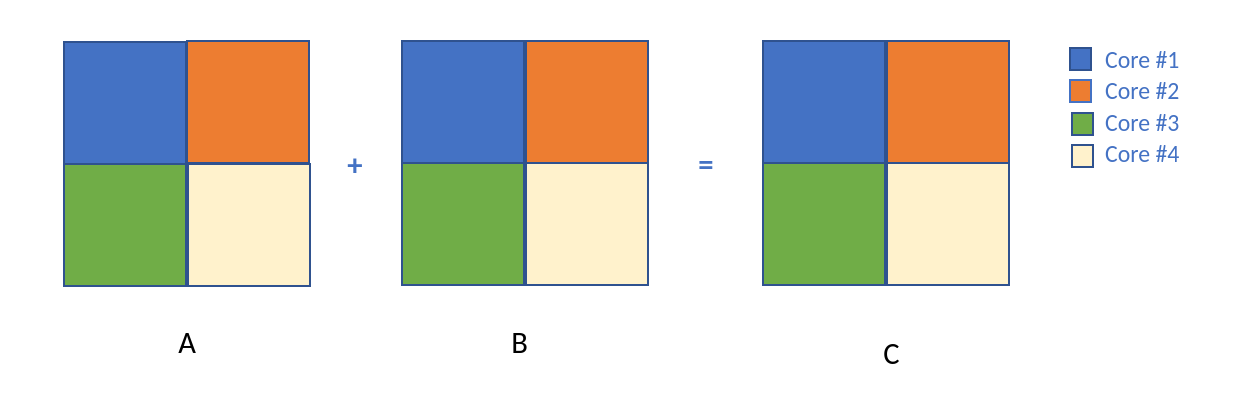
\includegraphics[width=0.72\linewidth]{images/old_backend.png}
			\caption{An example of how C=A+B is performed in parallel in Blaze with 4 cores}	
		\end{figure}	

	\end{outline}
\end{frame}

%\begin{frame}{Background}
%	\begin{outline}
%		\1 Effect of Task Granularity on execution time
%		\1 Universal Scalability Law
%	\end{outline}
%\end{frame}
%\begin{frame}{Background: Loop Scheduling}
%	\begin{outline}
%				\1Chunk size: Number of loop iterations executed by one thread 
%%				\1Static and dynamic loop scheduling
%			\begin{figure}[]
%			\centering
%			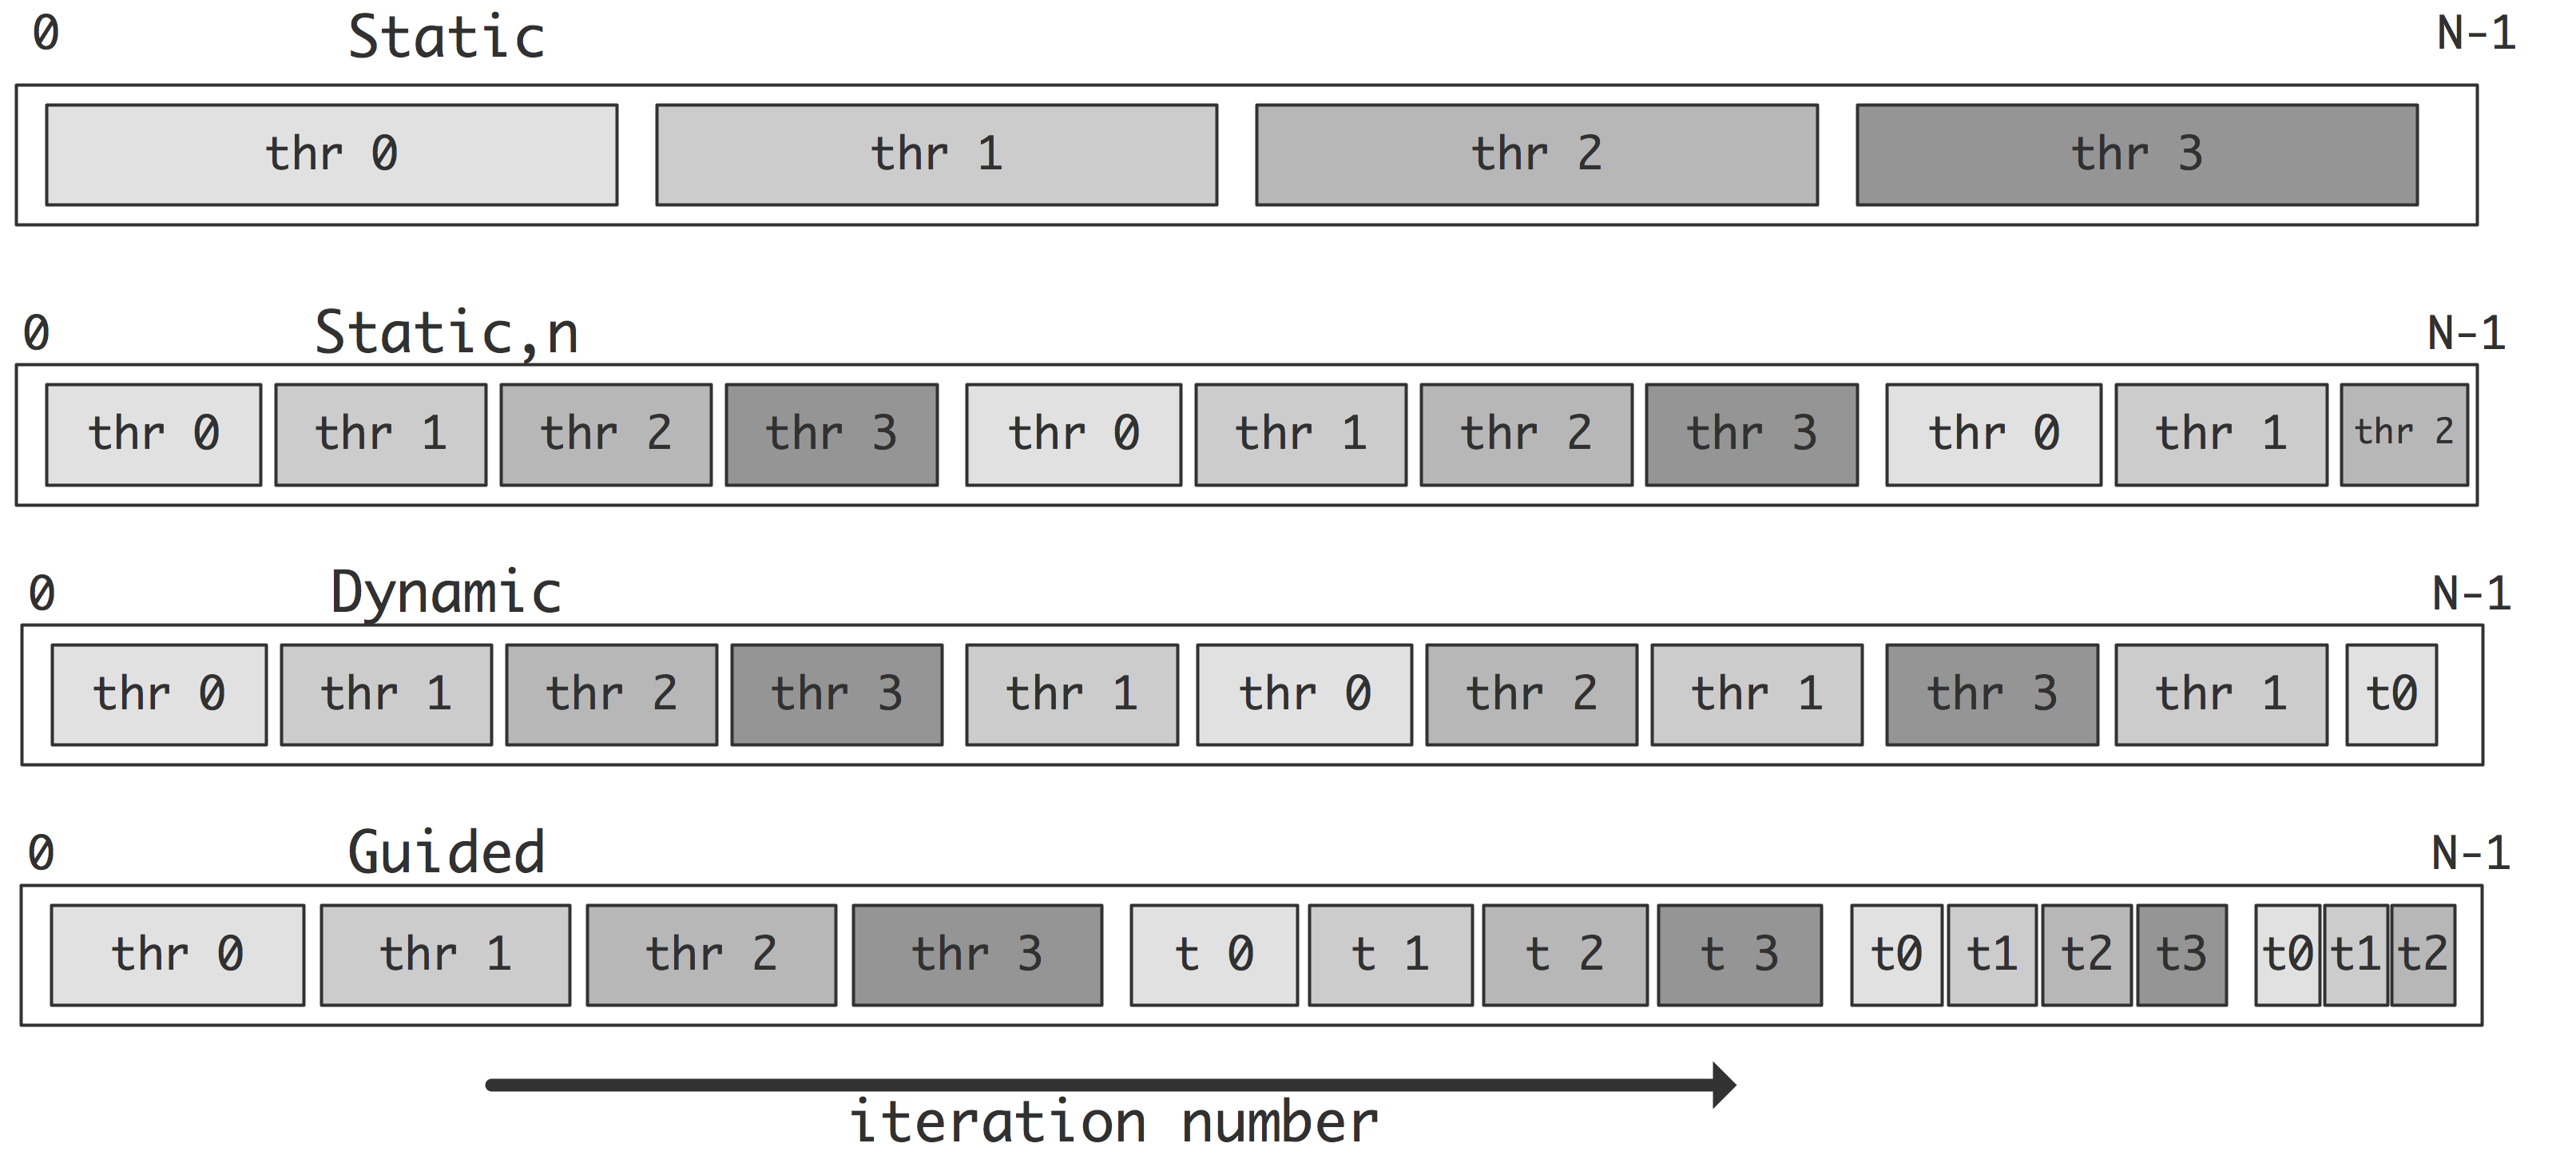
\includegraphics[scale=0.09]{images/schedules.png}
%				\caption{An example of different loop scheduling methods\footnote{http://pages.tacc.utexas.edu/~eijkhout/pcse/html/omp-loop.html}}
%%			\caption{An example of loop chunking\footnote{Ciorba, Florina M., Christian Iwainsky, and Patrick Buder. "OpenMP loop scheduling revisited: making a case for more schedules." International Workshop on OpenMP. Springer, Cham, 2018.}}	
%			\label{fig_loop}
%		\end{figure}
%	\end{outline}
%\end{frame}

%\begin{frame}{Background: Loop Scheduling}
%	\begin{outline}
%				\1Chunk size: Number of loop iterations executed by one thread 
%%				\1Static and dynamic loop scheduling
%			\begin{figure}[]
%			\centering
%			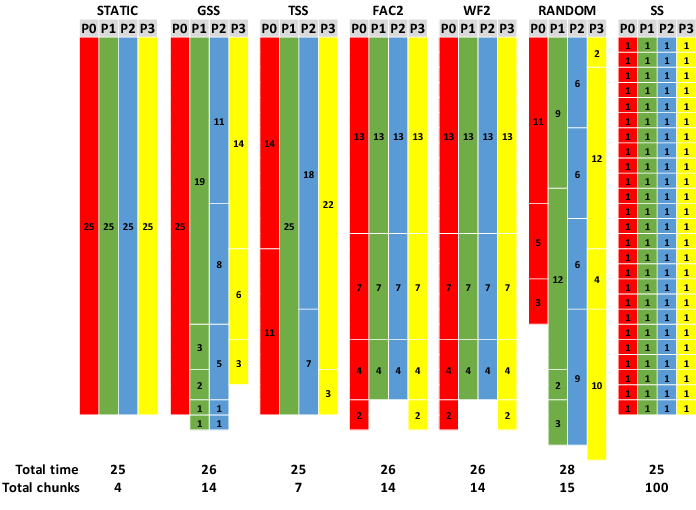
\includegraphics[scale=0.98]{images/loop_1.png}
%				\caption{An example of effect of different loop scheduling methods\footnote{Ciorba, F. M., Iwainsky, C., \& Buder, P. (2018, September). OpenMP loop scheduling revisited: making a case for more schedules. In International Workshop on OpenMP (pp. 21-36). Springer, Cham.}}
%%			\caption{An example of loop chunking\footnote{Ciorba, Florina M., Christian Iwainsky, and Patrick Buder. "OpenMP loop scheduling revisited: making a case for more schedules." International Workshop on OpenMP. Springer, Cham, 2018.}}	
%			\label{fig_loop}
%		\end{figure}
%	\end{outline}
%\end{frame}

%\begin{frame}{HPX Tasks}
%	\begin{outline}
%		
%	\end{outline}
%\end{frame}

\begin{frame}{Background: Task Granularity}
	\begin{outline}
		Grain size: The amount of work performed by one task
		\1What causes performance degradation?
		\2Overheads
		\2Starvation
		\begin{figure}
			\centering
			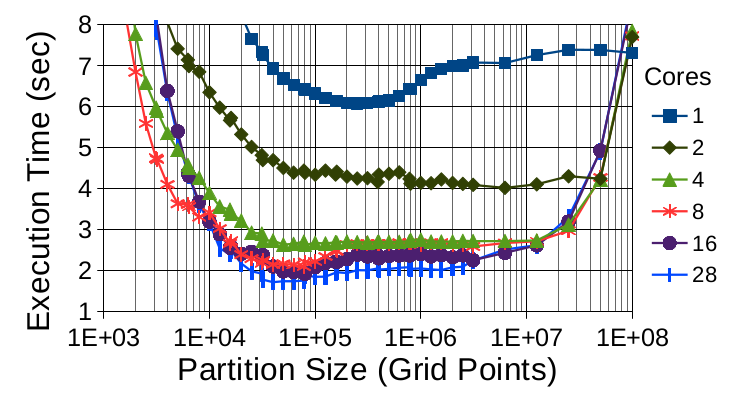
\includegraphics[width=0.72\linewidth]{images/task_granularity.png}
			\caption{The effect of task size on execution time for Stencil application\footnote{Grubel, Patricia, et al. "The performance implication of task size for applications on the hpx runtime system." 2015 IEEE International Conference on Cluster Computing. IEEE, 2015.}}	
	
		\end{figure}
		
	\end{outline}
\end{frame}




%\begin{frame}{Background: Modeling Performance based on number of cores: Other Models}
%	\begin{outline}
%		\1Quadratic model
%		$$ S(p) = p-\gamma{p(p-1)}$$
%		\1Exponential model
%		$$S(p) = p(1-\alpha)^{(p-1)}$$
%		\1Geometric model
%		$$S(p) = \frac{1-\phi^{p}}{1-\phi}$$
%	\end{outline}
%\end{frame}



%\begin{frame}{Definitions}
%	\begin{outline}
%	\1Block size
%	\1Chunk size
%	\1Grain size
%	\end{outline}
%\end{frame}
\section{Method}
\begin{frame}{Method: Objective}
	\begin{outline}
		Dynamically divide the work among the cores based on number of cores, matrix size, complexity of the operation, machine architecture.
		For this purpose two parameters have been introduced:
		\1block\textunderscore size: at each loop iteration the assignment is performed on one block
		\1chunk\textunderscore size: the number of loop iterations included in one task 
		\begin{figure}
			\centering
			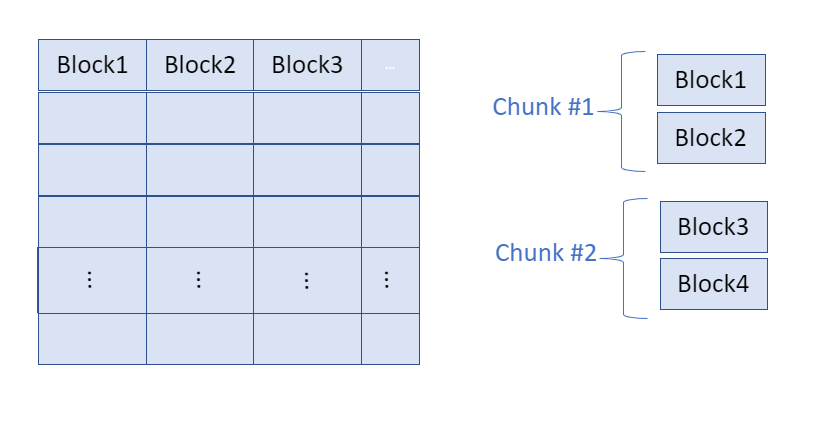
\includegraphics[width=0.72\linewidth]{images/chunks.png}
			\caption{An example of blocking a matrix and creating chunks for chunk\textunderscore size = 2}	
		\end{figure}	
	\end{outline}
\end{frame}

\begin{frame}{Method: Data Collection}
	\begin{outline}
		\1Starting from DMATDMATADD benchmark: $C=A+B$
	\begin{table}[H]
		\centering
		\resizebox{0.8\textwidth}{!}
		{\begin{tabular}{|c | c |} 
				\hline
				Category & Configuration \\
				\hline
				\hline
				Matrix sizes & 200, 230, 264, 300, 396, 455, 523, 600, 690, 793, 912, 1048, 1200, 1380, 1587 \\ [0.5ex] 
				\hline
				Number of cores & 1, 2, 3, 4, 5, 6, 7, 8 \\ 	
				\hline
				Number of rows in the block & 4, 8, 12, 16, 20, 32 \\
				\hline	
				Number of columns in the block & 64, 128, 256, 512, 1024 \\
				\hline
				Chunk size & Between 1 and total number of blocks (logarithmic increase)\\\hline
		\end{tabular}}
		
		\caption{List of different values used for each variable for running the $DMATDMATADD$ benchmark}
		\label{table1}
	\end{table}
	\end{outline}
\end{frame}


\begin{frame}{Method: Data Analysis}
	\begin{outline}
		\1For simplicity we look at each matrix size individually, one number of core at a time 
		
		
		\begin{figure}
			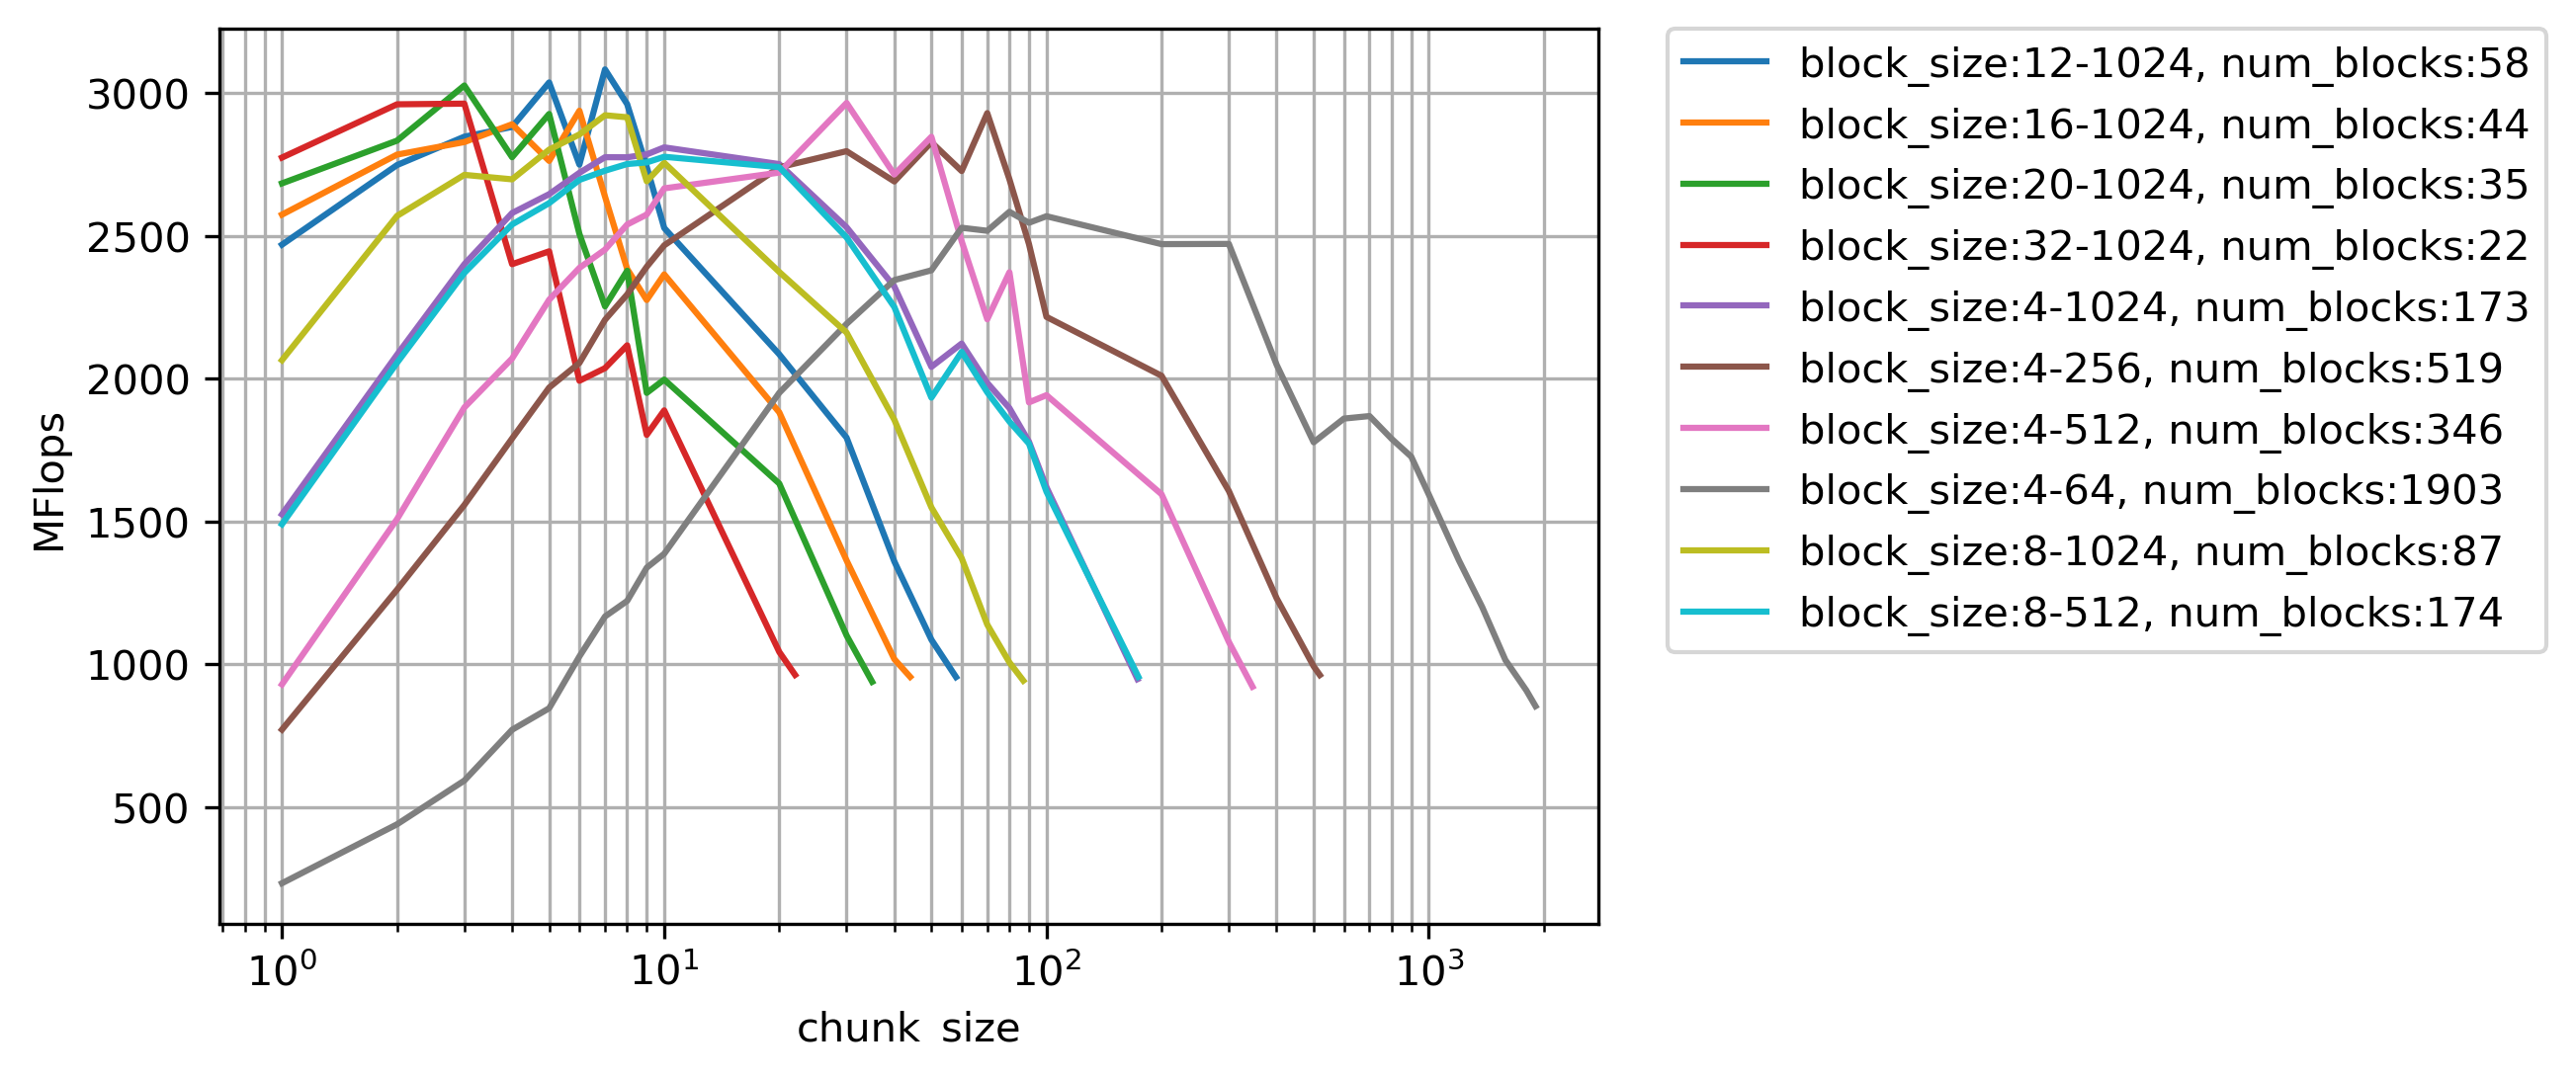
\includegraphics[width=0.9\linewidth]{images/fig5.png}	
			\caption{The results obtained from running $DMATDMATADD$ benchmark for matrix sizes 690$\times$690 with different combinations of block size and chunk size on $4$ cores}	
		\end{figure}
	\end{outline}
\end{frame}


\begin{frame}{Method: Observation}
	\begin{outline}
		\begin{figure}
			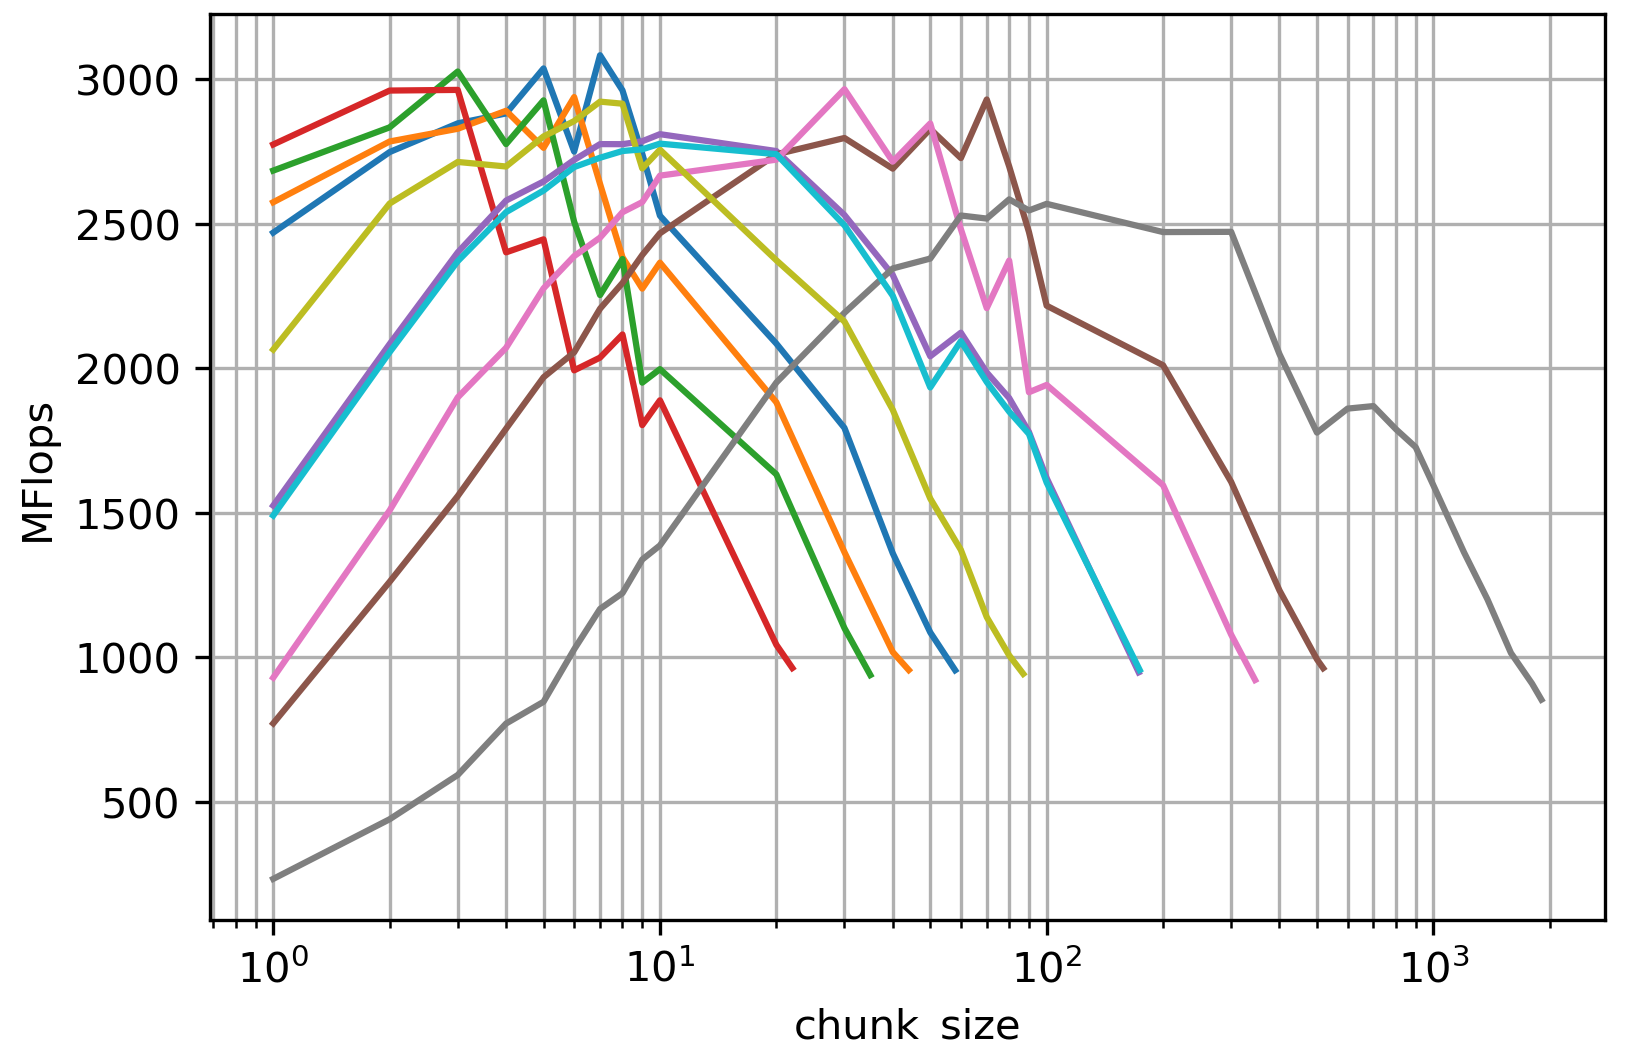
\includegraphics[scale=0.2]{images/fig5_cropped.png}			
		\end{figure}
		\1For each selected block size, there is a range of chunk sizes that gives us the best performance. 
		\1Except for some uncommon cases, no matter which block size we choose, we are able to achieve the maximum performance if we select the right chunk size.  
		\pause
		\1Instead of looking at block size and chunk size individually, look at grain size.
	\end{outline}
\end{frame}

\begin{frame}{Method: Throughput vs. Grain Size}
	\begin{outline}
		Grain size: The number of floating point operations performed by one thread\\
		\1Grain size represents the complexity of the expression
		\1For $DMATDMATADD$, with $block\textunderscore{size}=r\times{c}$ and  $chunk\textunderscore{size}=ch$ \\ Grain\textunderscore{size}=$r\times{c}\times{ch}$
		\begin{figure}[H]
			\centering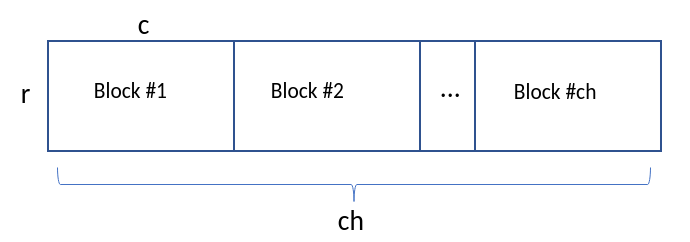
\includegraphics[width=1\linewidth]{images/grain_size.png}
			
			\label{fig28}
		\end{figure}
	
	\end{outline}
\end{frame}

\begin{frame}{Method: Throughput vs. Grain Size}
	\begin{outline}
		\begin{figure}[H]
			\centering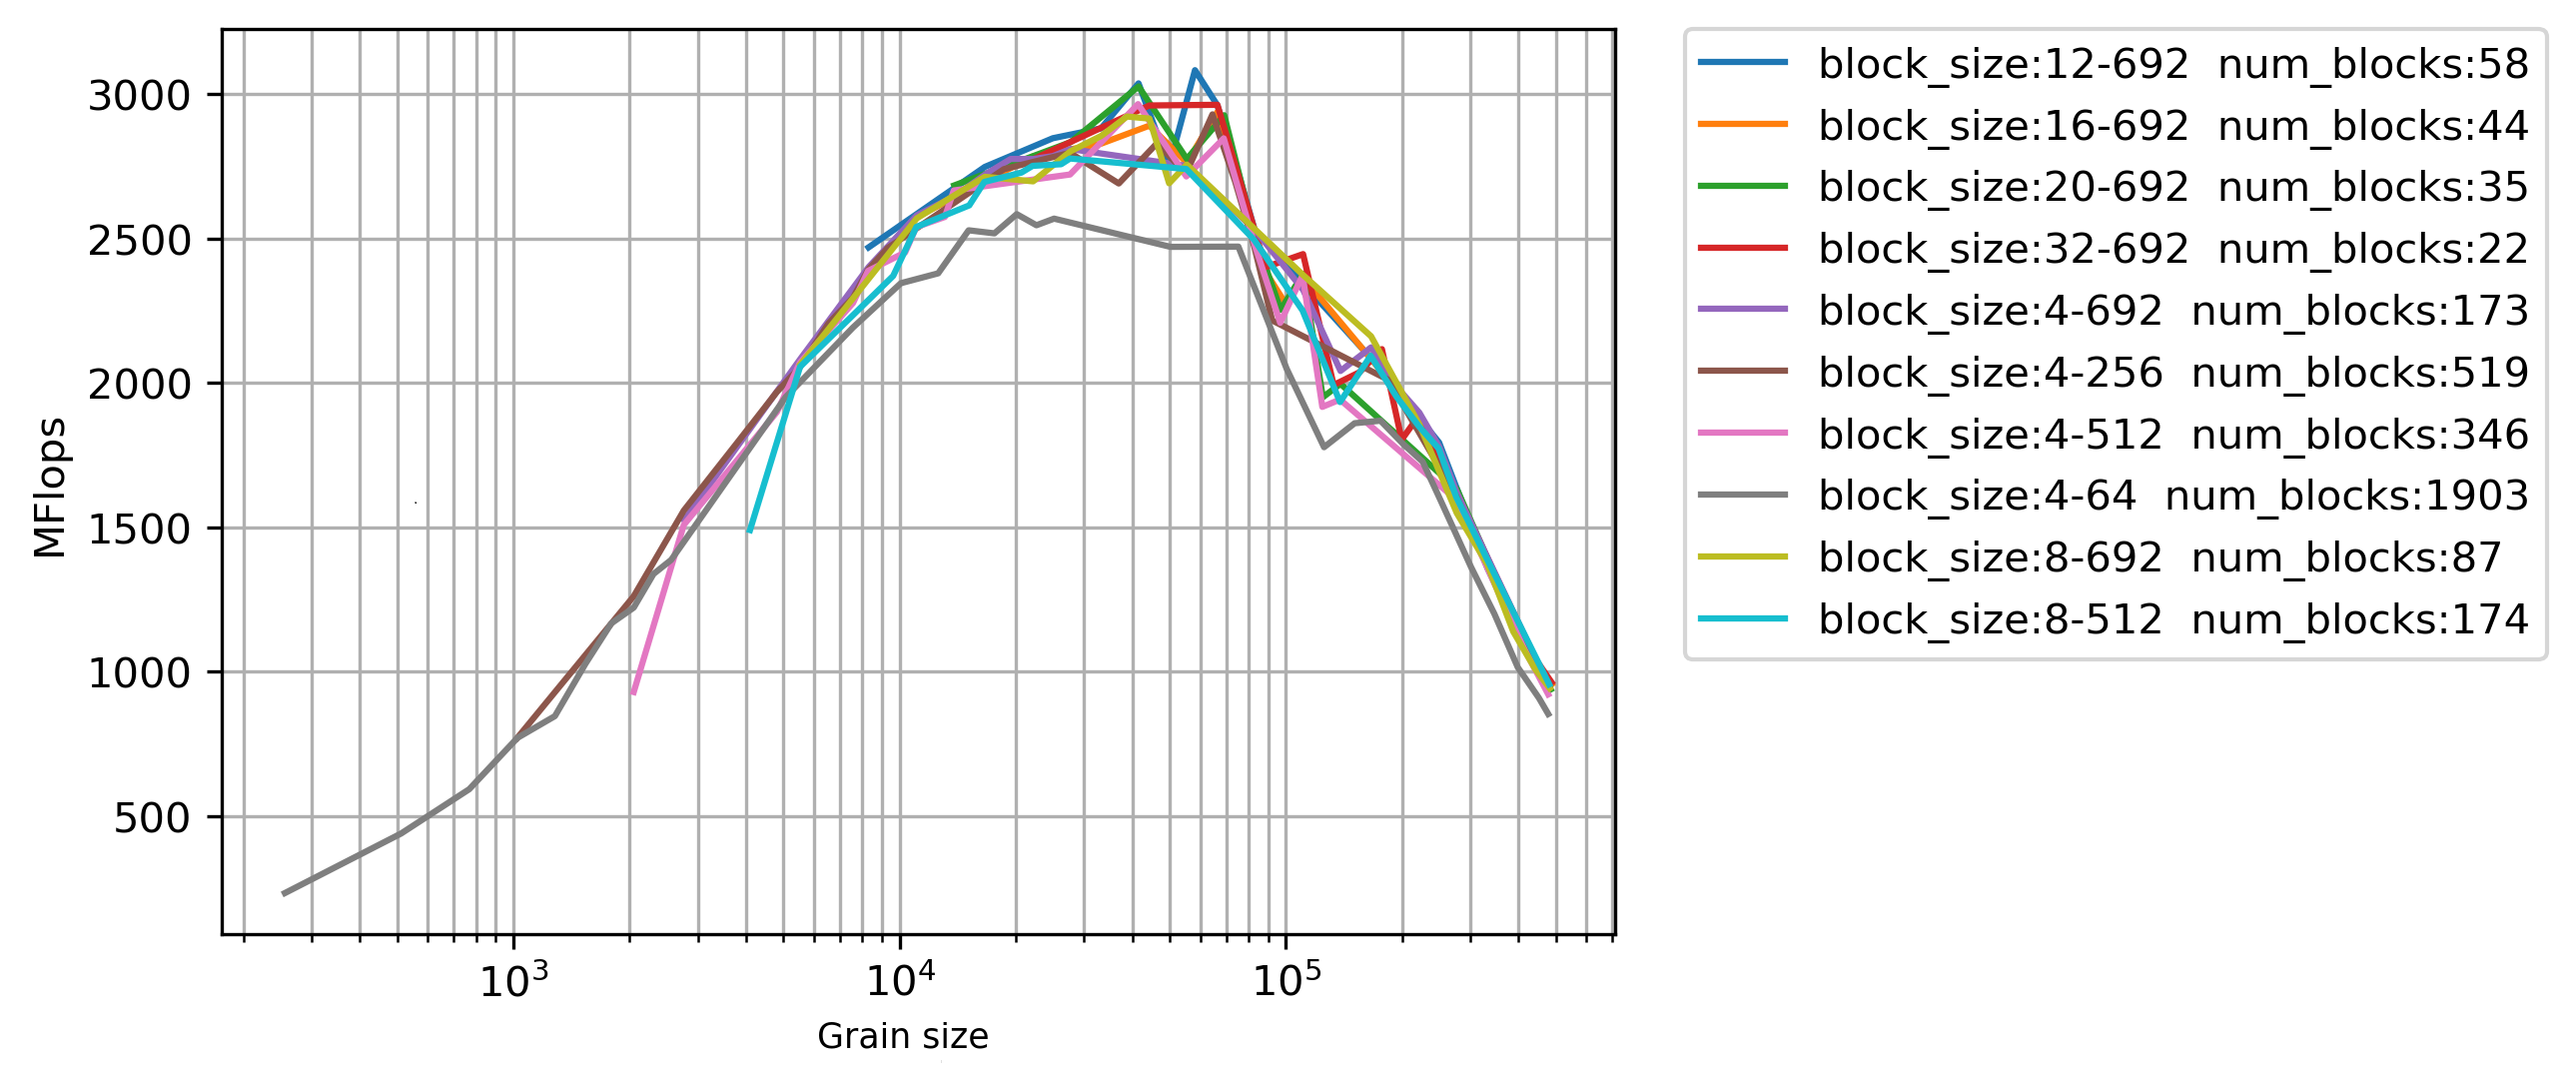
\includegraphics[width=1\linewidth]{images/fig6.png}
			\caption{The results obtained from running $DMATDMATADD$ benchmark through Blazemark for matrix size 690$\times$690 on $4$ cores.}	
			\label{fig6}
		\end{figure}
	
	\end{outline}
\end{frame}

\begin{frame}{Method: Throughput vs. Grain Size}
	\begin{outline}		
		The range of grain size for maximum performance
		\begin{figure}[H]
			\centering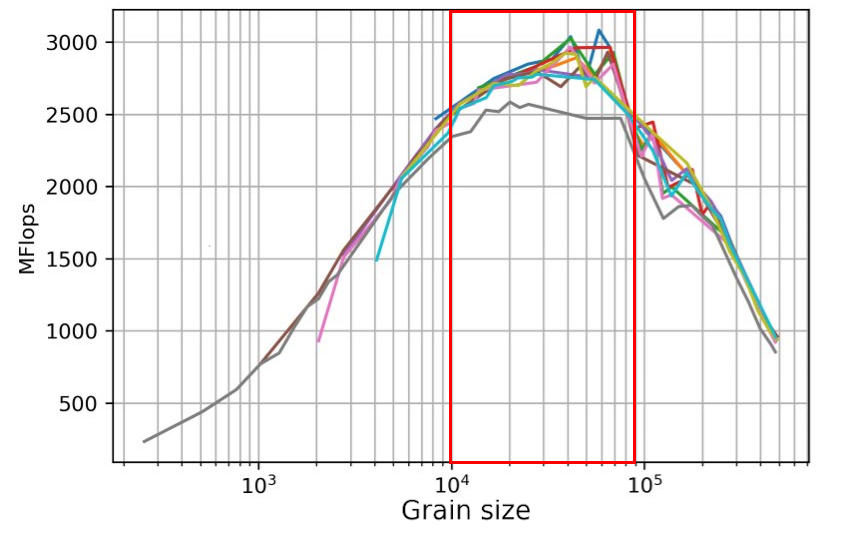
\includegraphics[scale=0.9]{images/fig6_range.png}
			\caption{The results obtained from running $DMATDMATADD$ benchmark through Blazemark for matrix size 690$\times$690 on $4$ cores.}	
			\label{fig7}
		\end{figure}
		
	\end{outline}
\end{frame}

\begin{frame}{Throughput vs. Grain Size and Number of Cores}
	\begin{outline}
		\begin{figure}[H]
			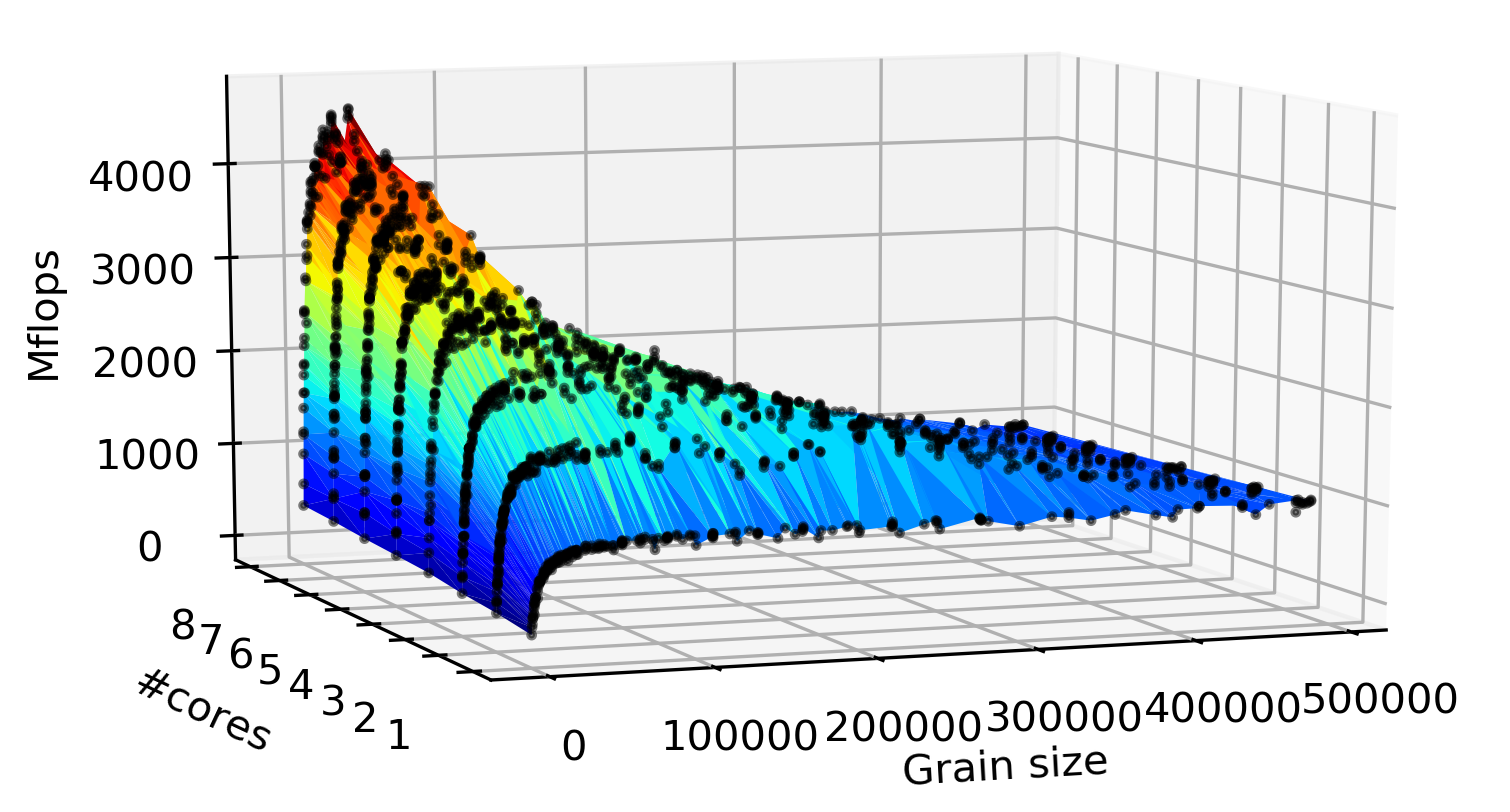
\includegraphics[scale=0.42]{images/fig2.png}					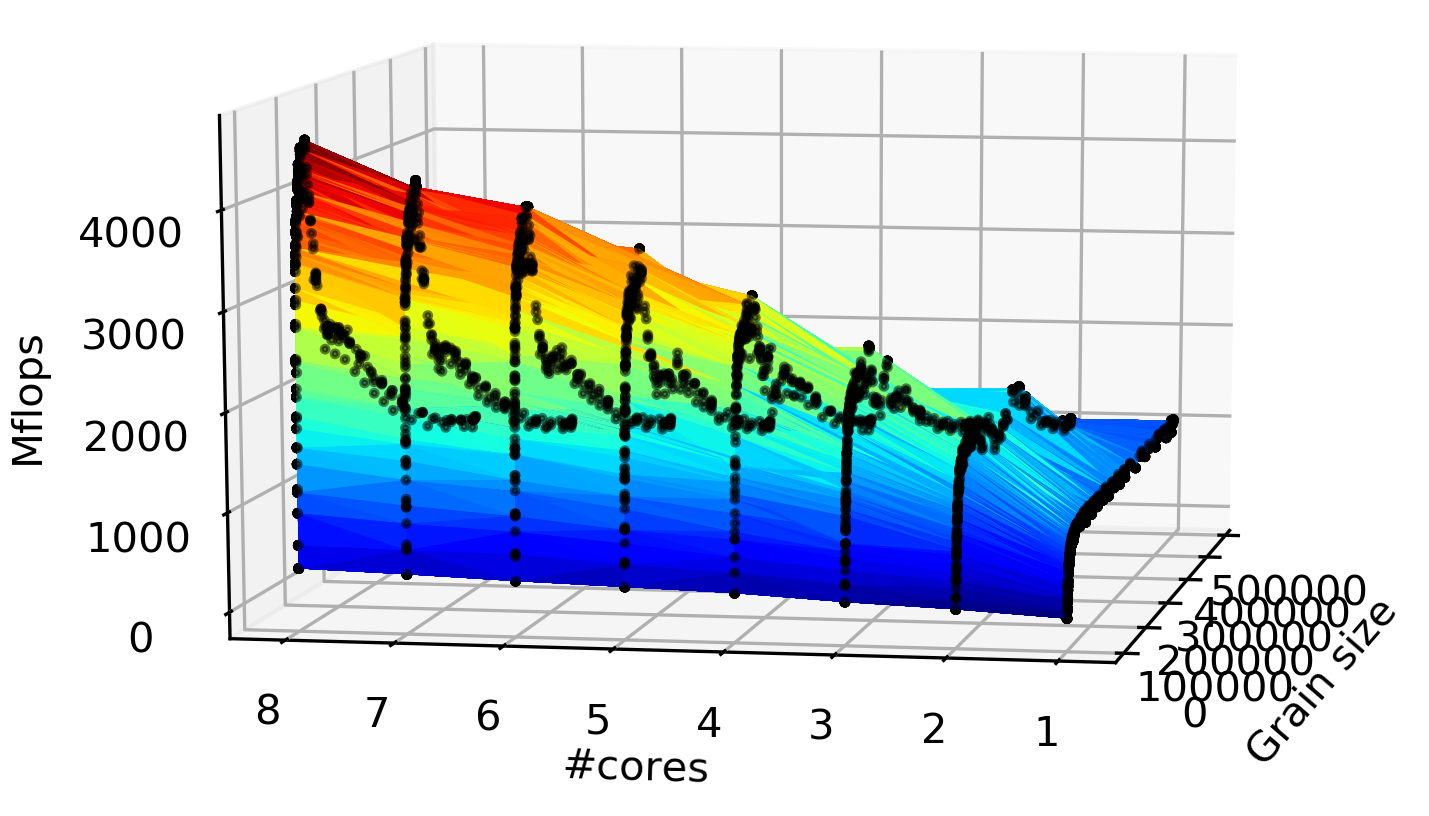
\includegraphics[scale=0.42]{images/fig3.png}
			\caption{The results obtained from running $DMATDMATADD$ benchmark through Blazemark for matrix size 690$\times$690 based on grain size and number of cores.}	
			\label{fig29}
		\end{figure}
\pause
	Can we model the relationship between the \textbf{throughput} and the \textbf{grain size} and the \textbf{number of cores}?
\pause	
\1First we try to model the relationship between throughput and grain size.
\pause	
\2Polynomial Model
\end{outline}
\end{frame}

%\begin{frame}{Throughput vs. Grain Size and Number of Cores}
%	\begin{outline}
%%		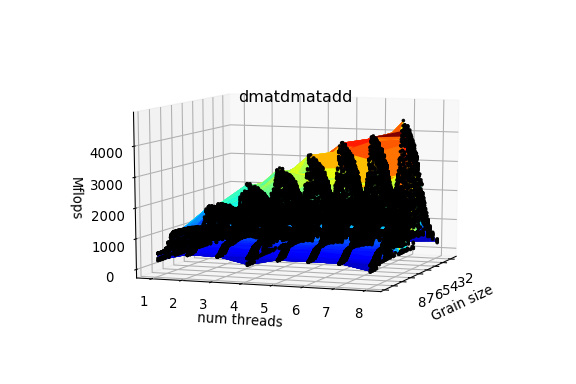
\includegraphics[scale=0.4]{images/fig1.png}	\\
%		Can we model the relationship between the \textbf{throughput} and the \textbf{grain size} and the \textbf{number of cores}?
%		\pause	
%		\1First we try to model the relationship between throughput and grain size.
%		\pause	
%		\2Polynomial Model
%
%	\end{outline}
%\end{frame}

%\begin{frame}{Modeling}
%	\begin{outline}
%		\1Polynomial Model
%		\1Bathtub Model
%	\end{outline}
%\end{frame}

\begin{frame}{Method: Polynomial Model}
	\begin{outline}
		
		In order to simplify the process and eliminate the effect of different possible factors, we started with limiting the problem to a fixed matrix size.	
		\1Used a second order polynomial to model the relationship between the throughput and the grain size when number of cores is fixed.
		\begin{columns}		
			\column{0.38\linewidth}
		 \centering$P=ag^2+bg+c$ 
		 \column{0.38\linewidth}  
		 \begin{figure}[]
		 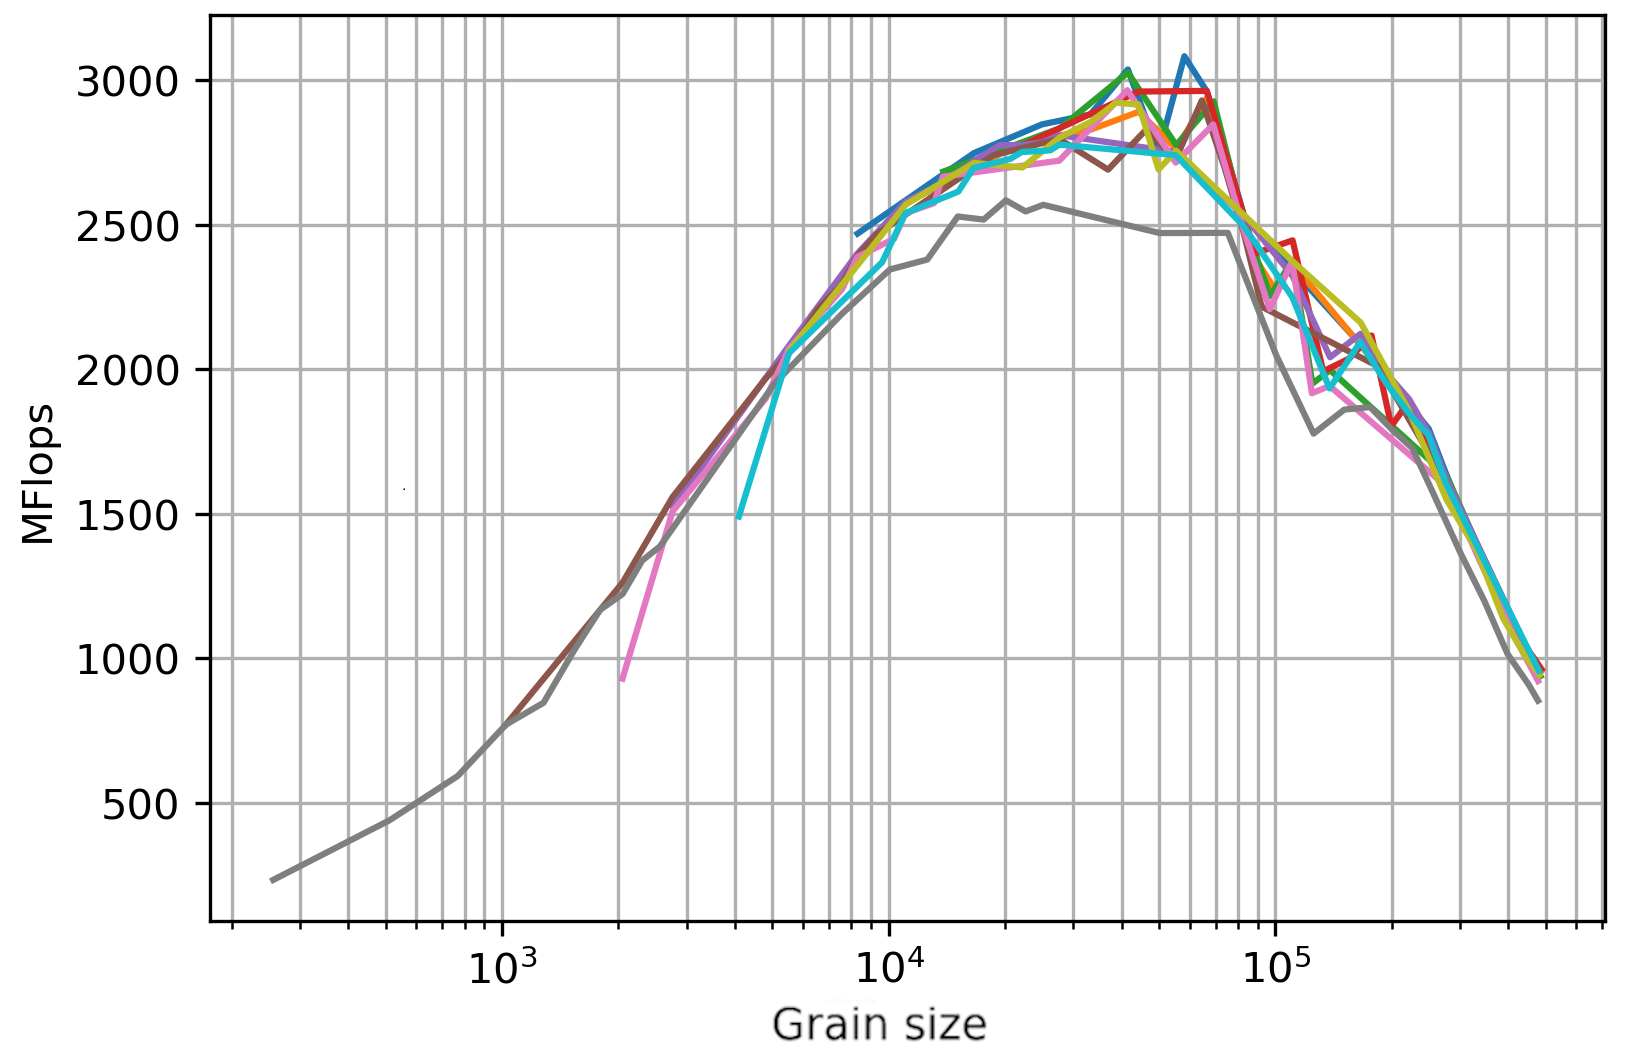
\includegraphics[scale=0.15]{images/fig6_cropped.png}
		 \end{figure}
		 
		\end{columns}
	\1Divide the data into training(60\%) and test(40\%)
	\end{outline}
\end{frame}

\begin{frame}{Method: Modeling Performance based on Grain Size}
	\begin{outline}	
		\begin{figure}[H]
			\centering
			\subfloat[1 core]{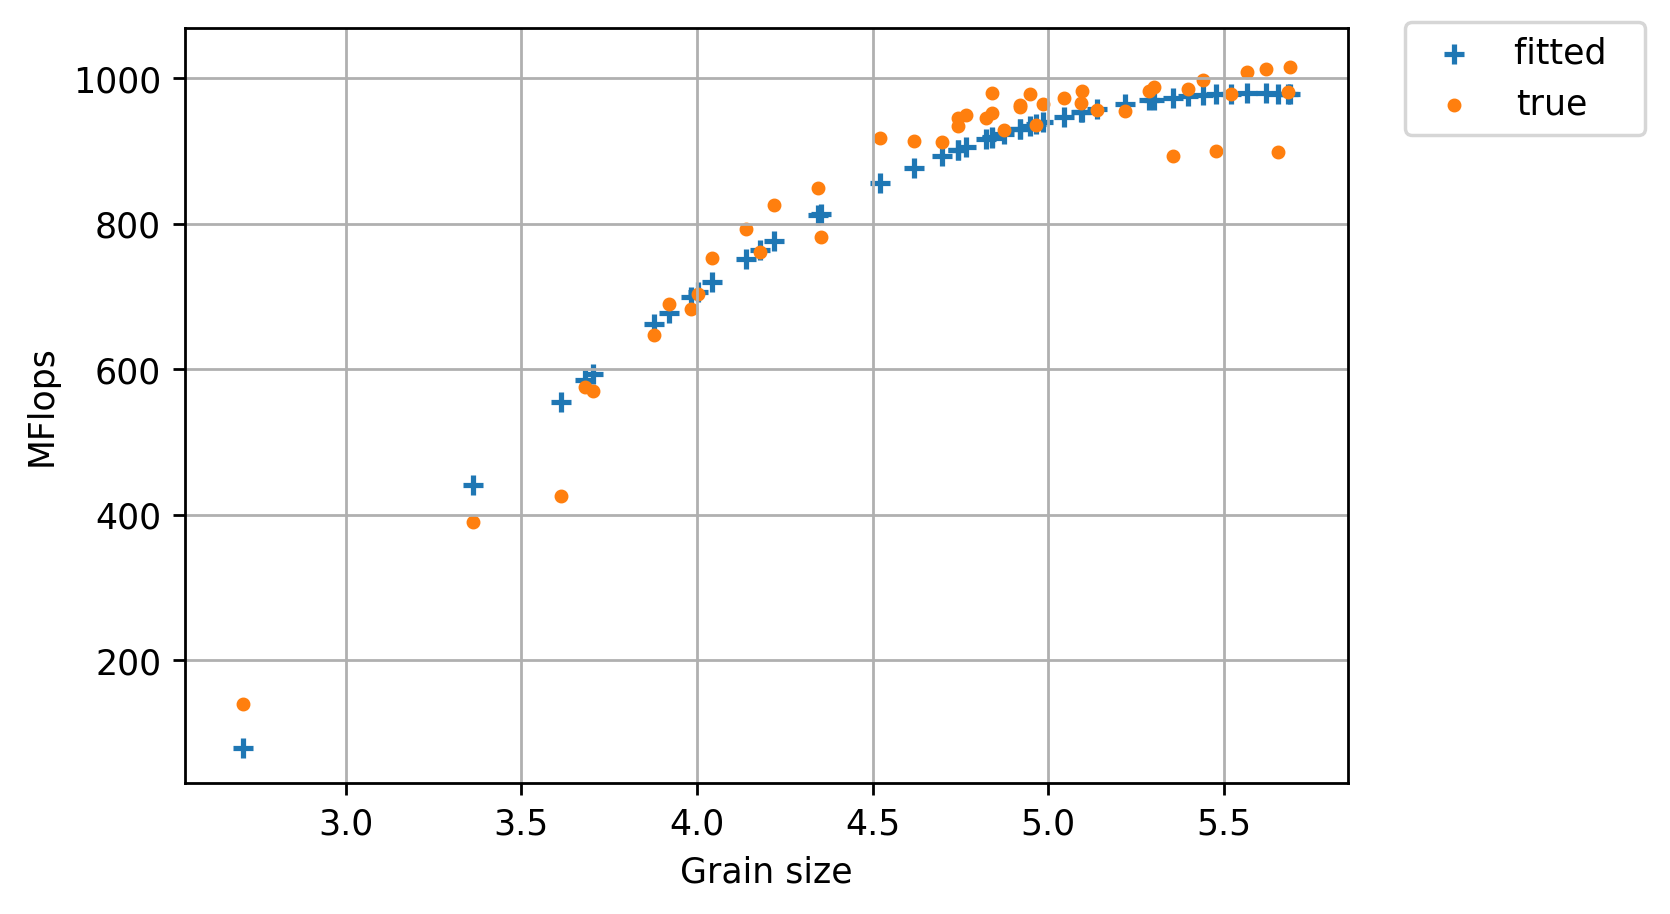
\includegraphics[scale=.3]{images/polyfit/fig_1_690.png}\label{fig10:a}}
			\subfloat[2 cores]{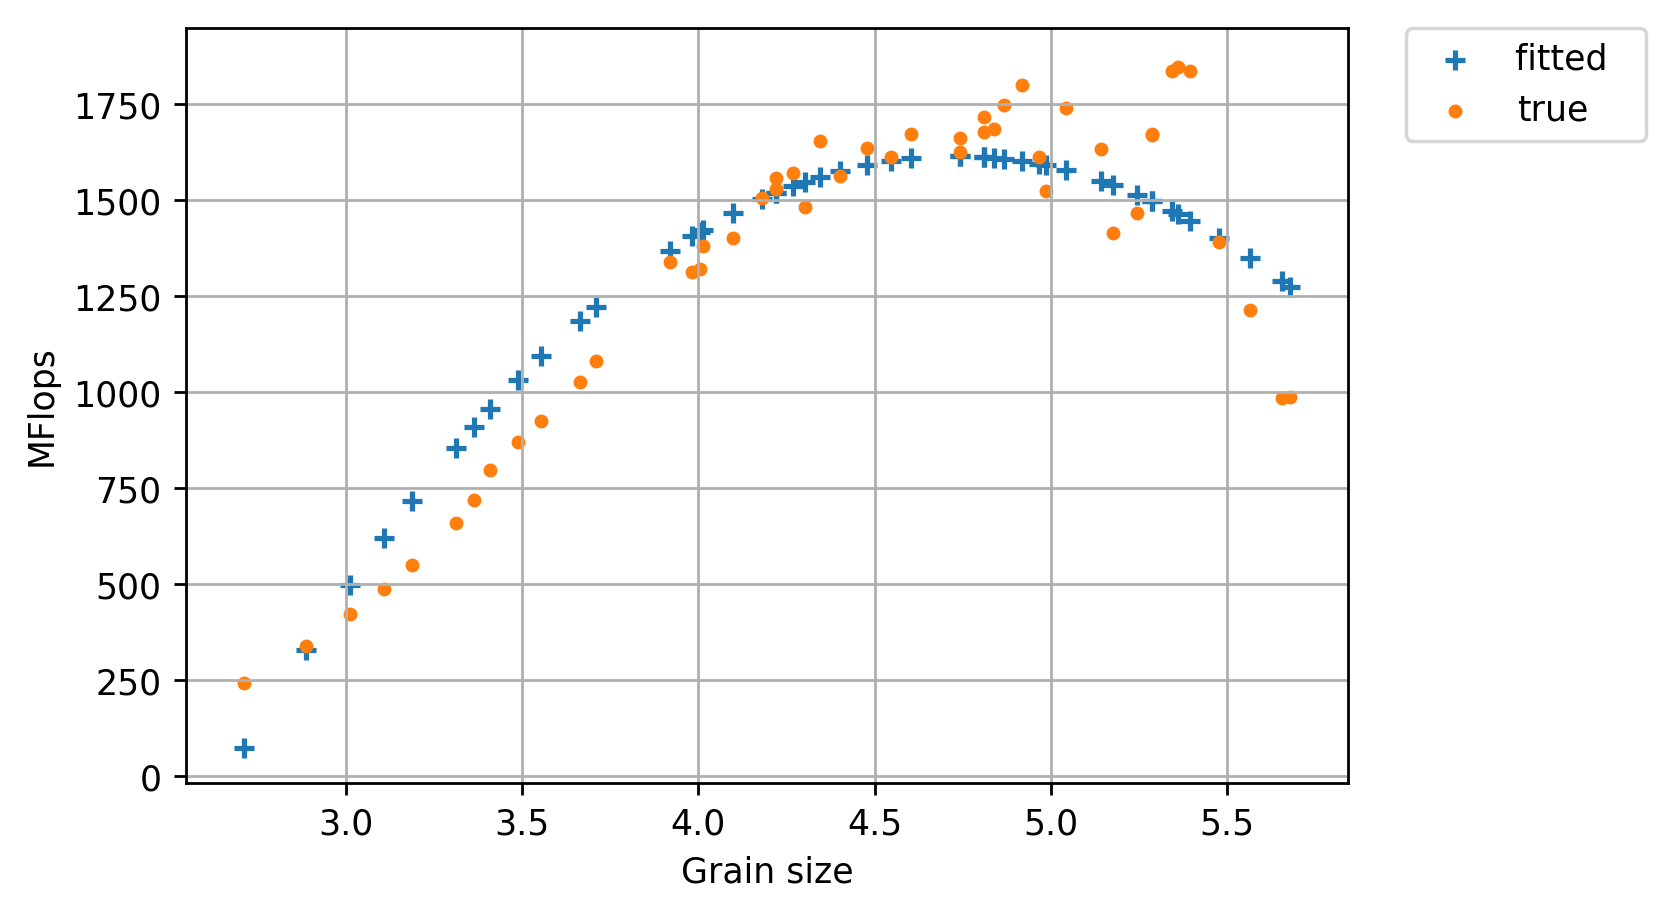
\includegraphics[scale=.3]{images/polyfit/fig_2_690.png}\label{fig10:b}}\hfill
%			\subfloat[3 cores]{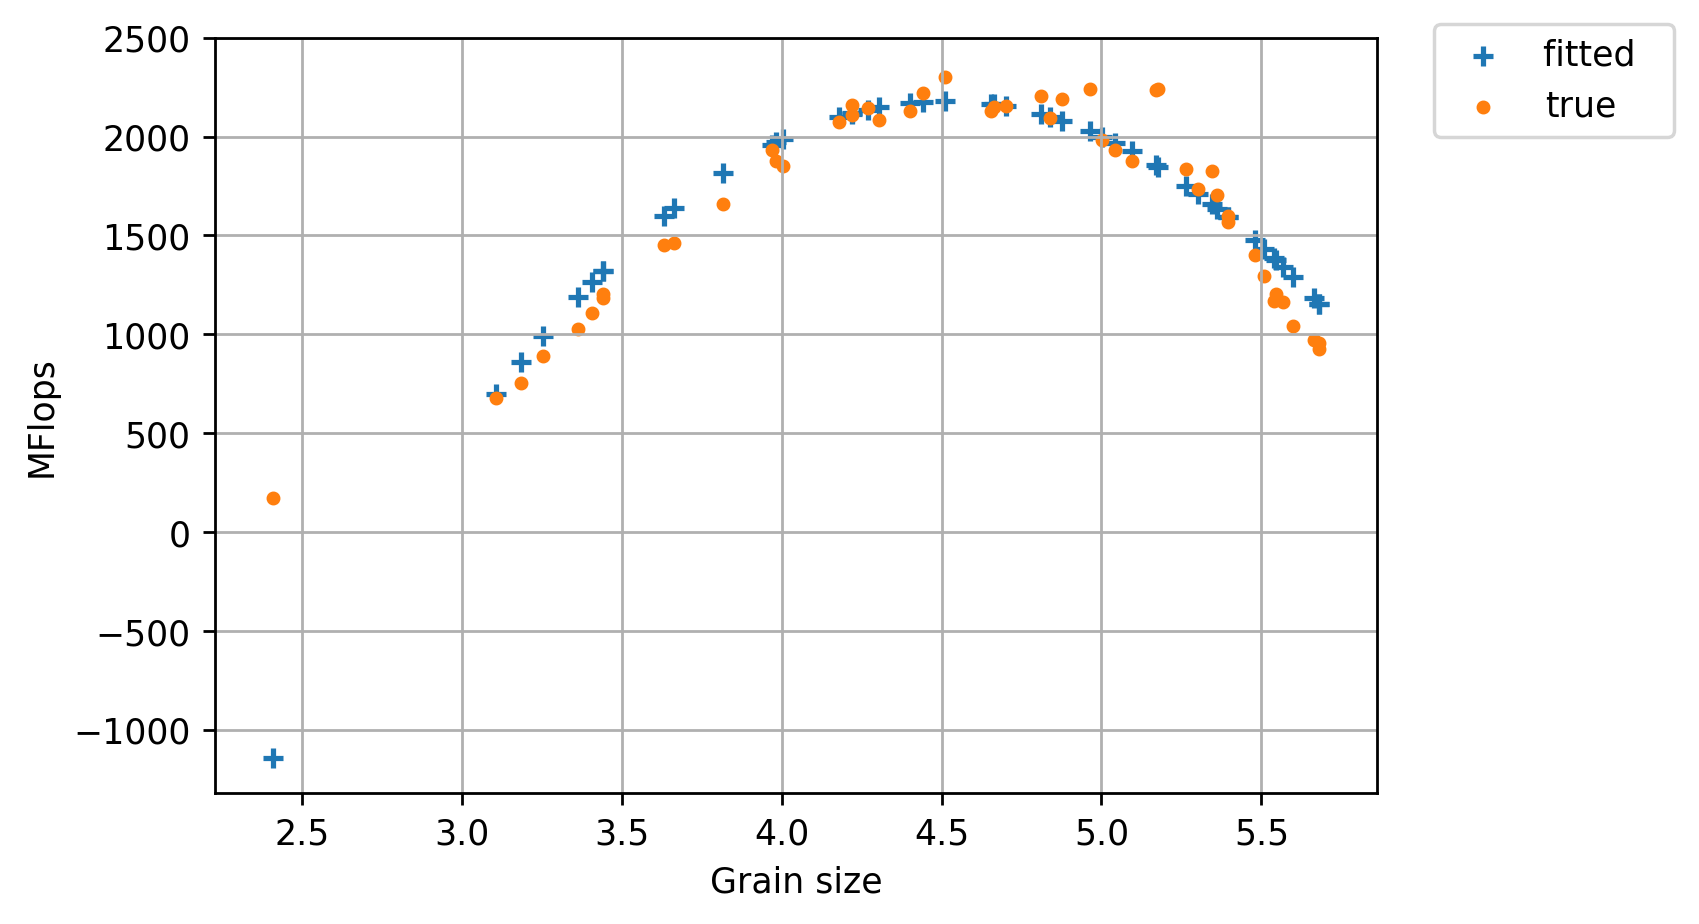
\includegraphics[scale=.18]{images/polyfit/fig_3_690.png}\label{fig10:c}}{\hfill}
			\subfloat[4 cores]{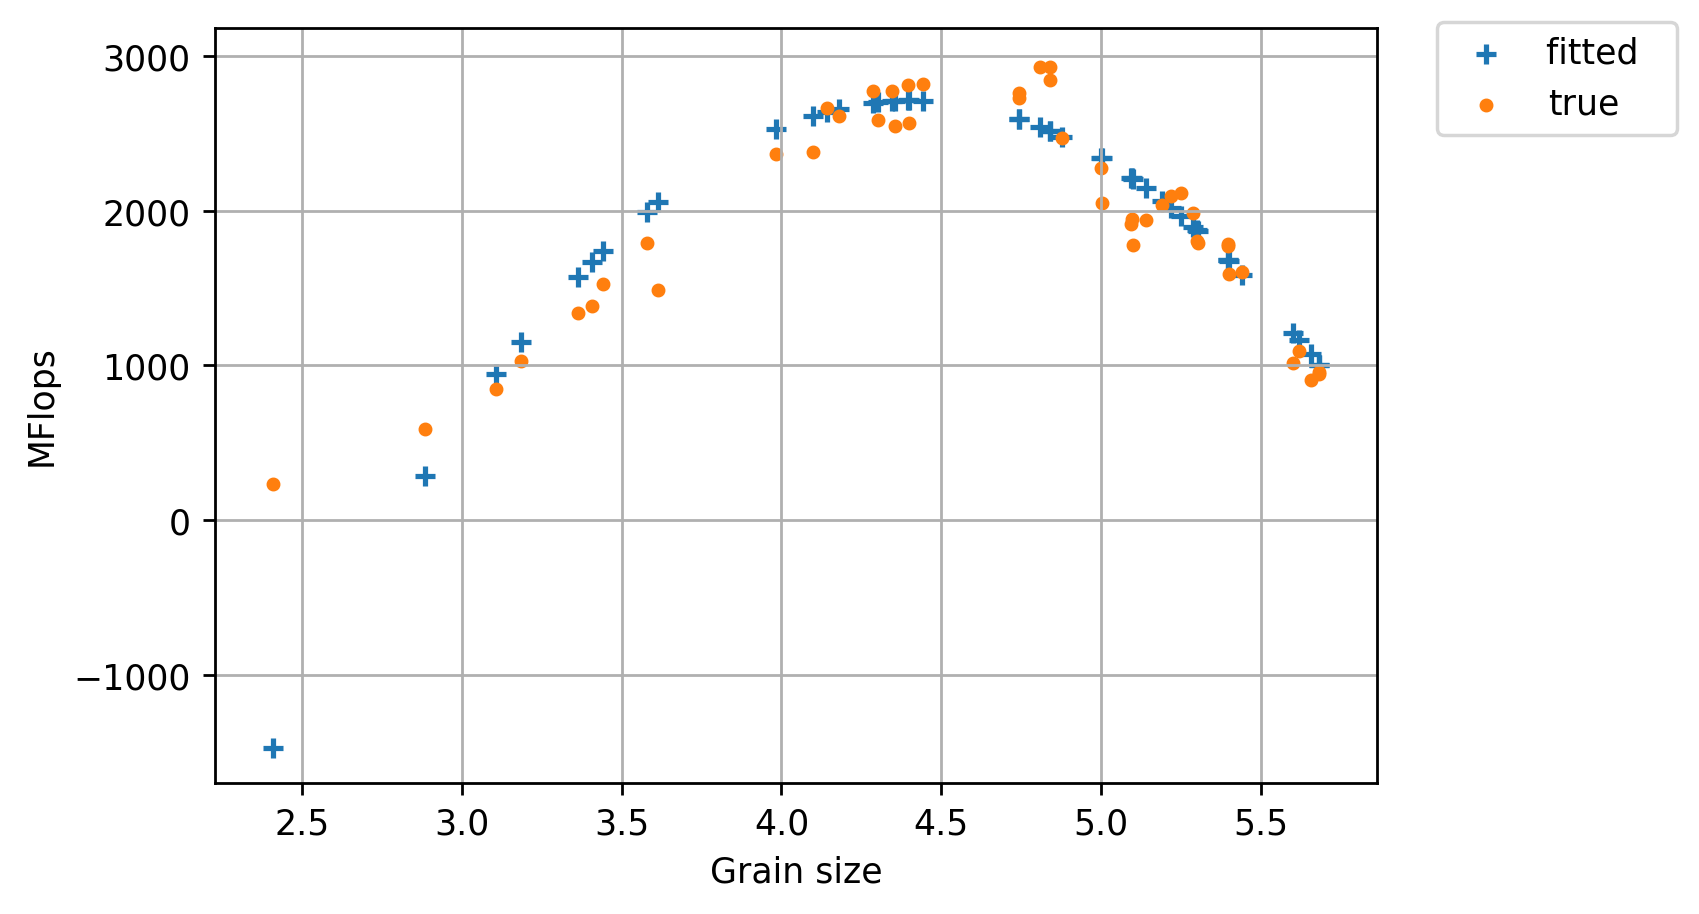
\includegraphics[scale=.3]{images/polyfit/fig_4_690.png}\label{fig10:d}}
%			\subfloat[5 cores]{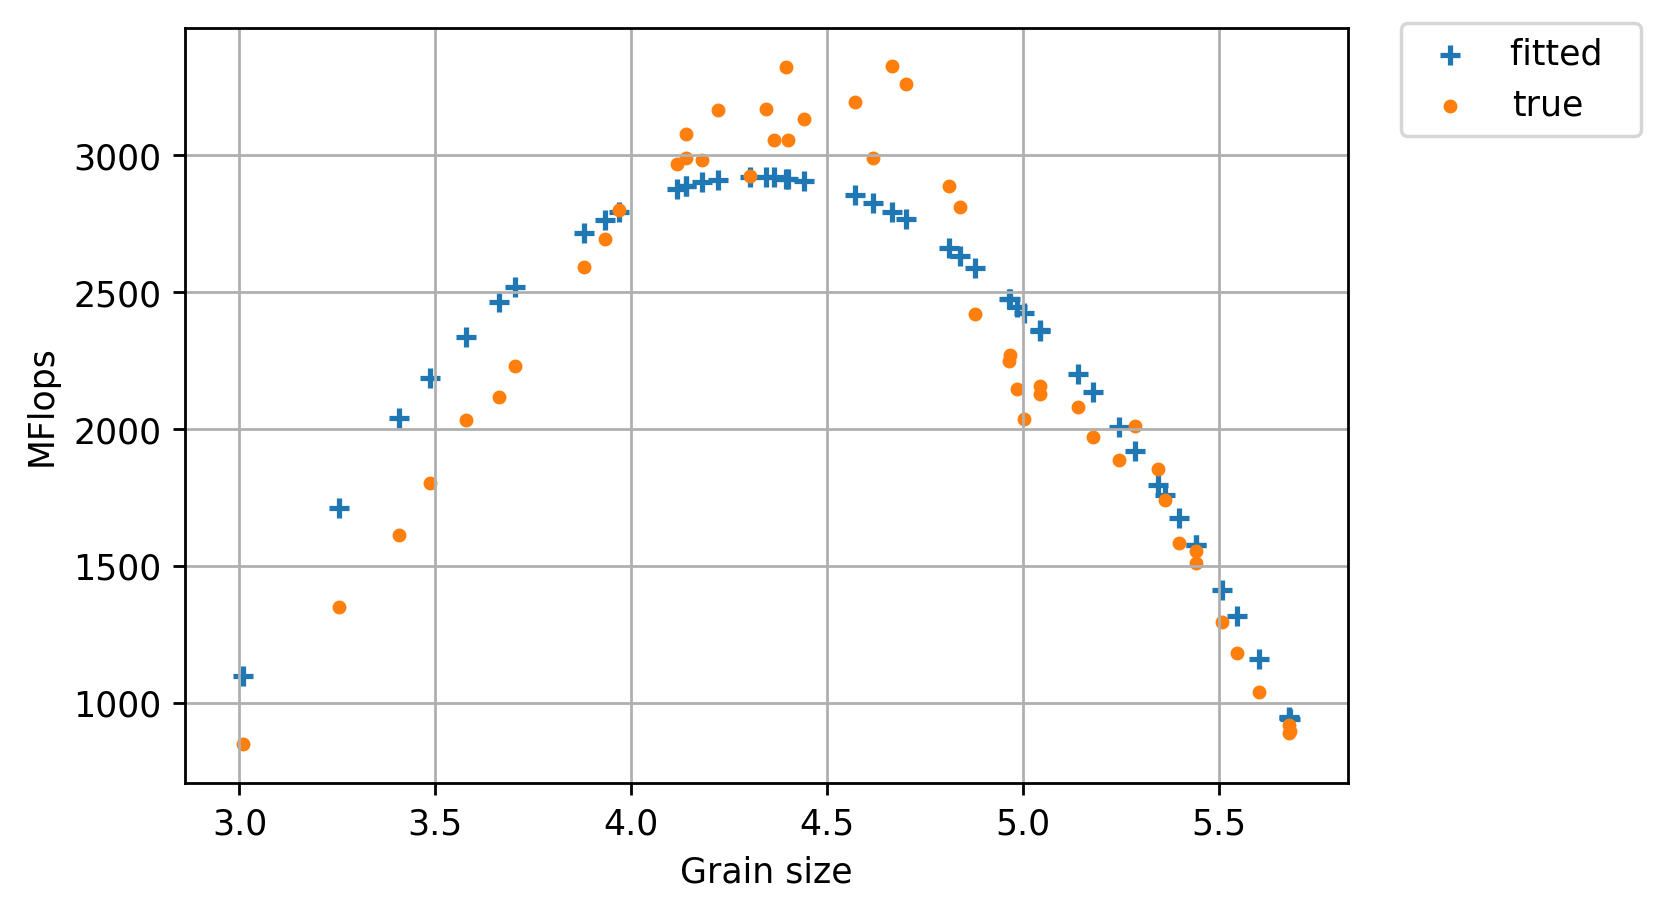
\includegraphics[scale=.18]{images/polyfit/fig_5_690.png}\label{fig10:e}}
%			\subfloat[6 cores]{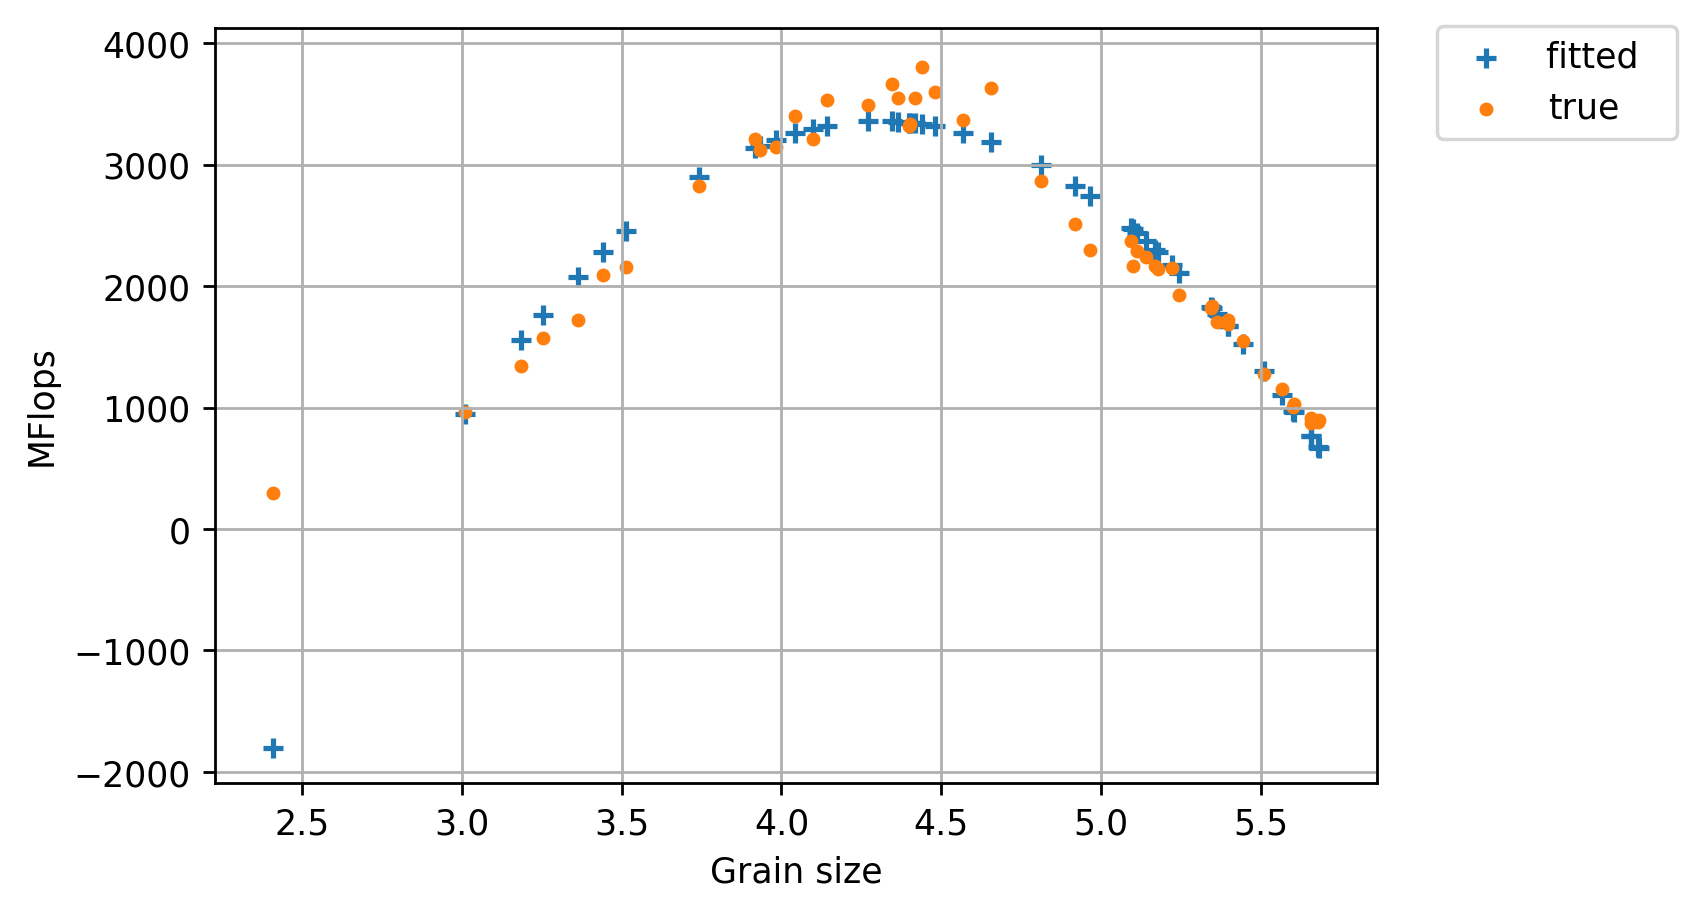
\includegraphics[scale=.18]{images/polyfit/fig_6_690.png}\label{fig10:f}}{\hfill}
%			\subfloat[7 cores]{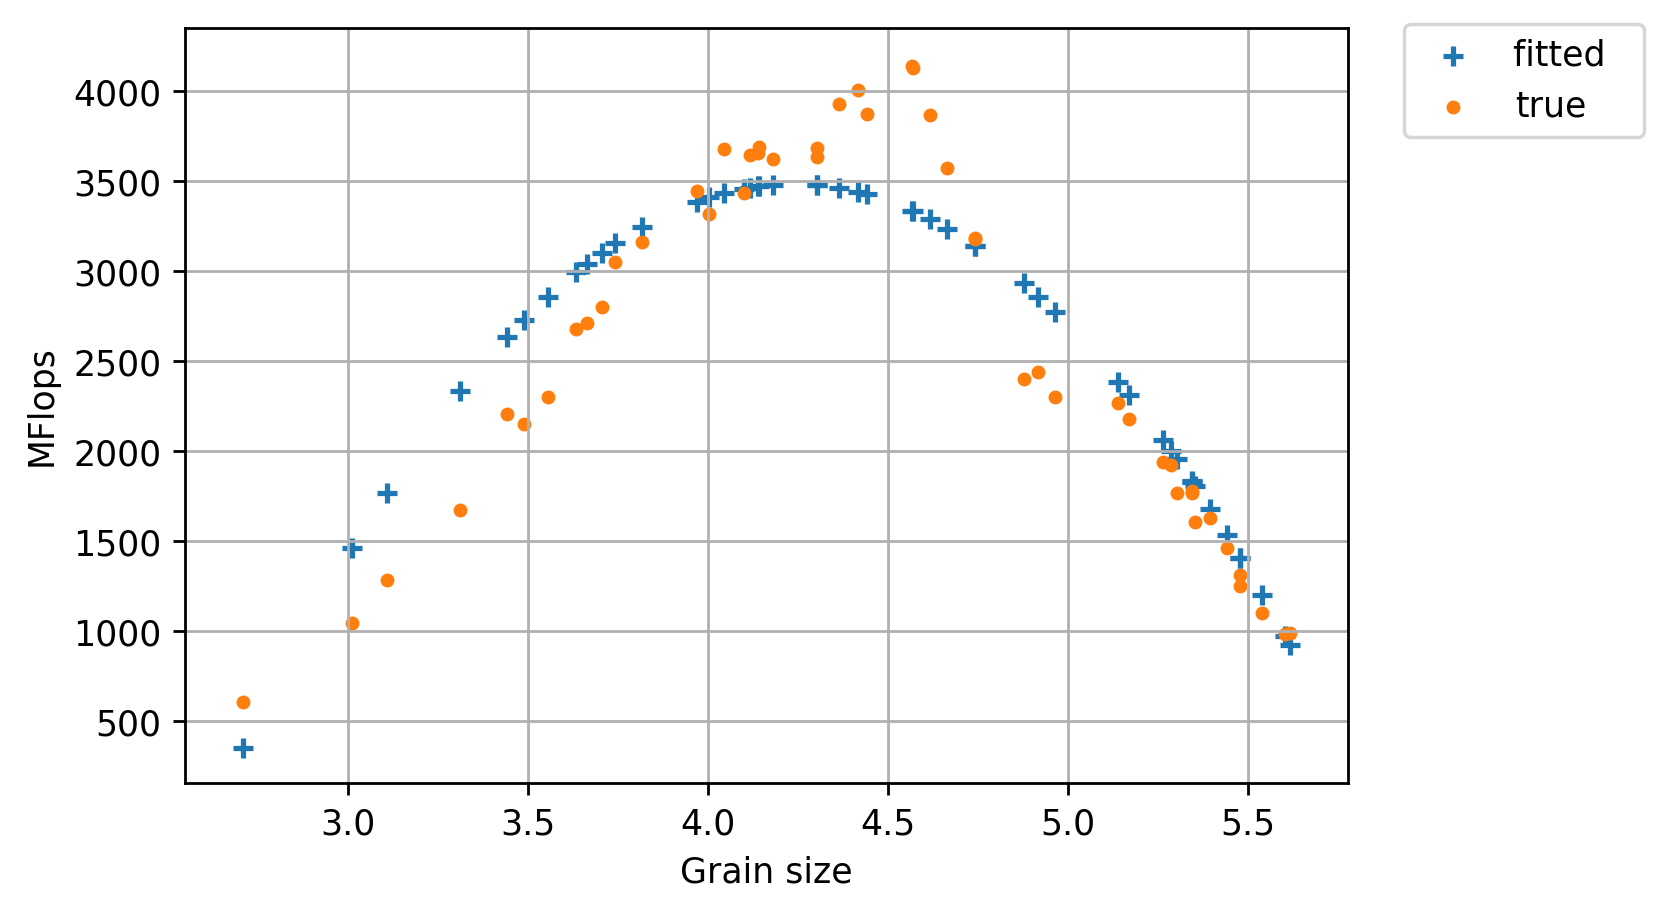
\includegraphics[scale=.18]{images/polyfit/fig_7_690.png}\label{fig10:g}}
			\subfloat[8 cores]{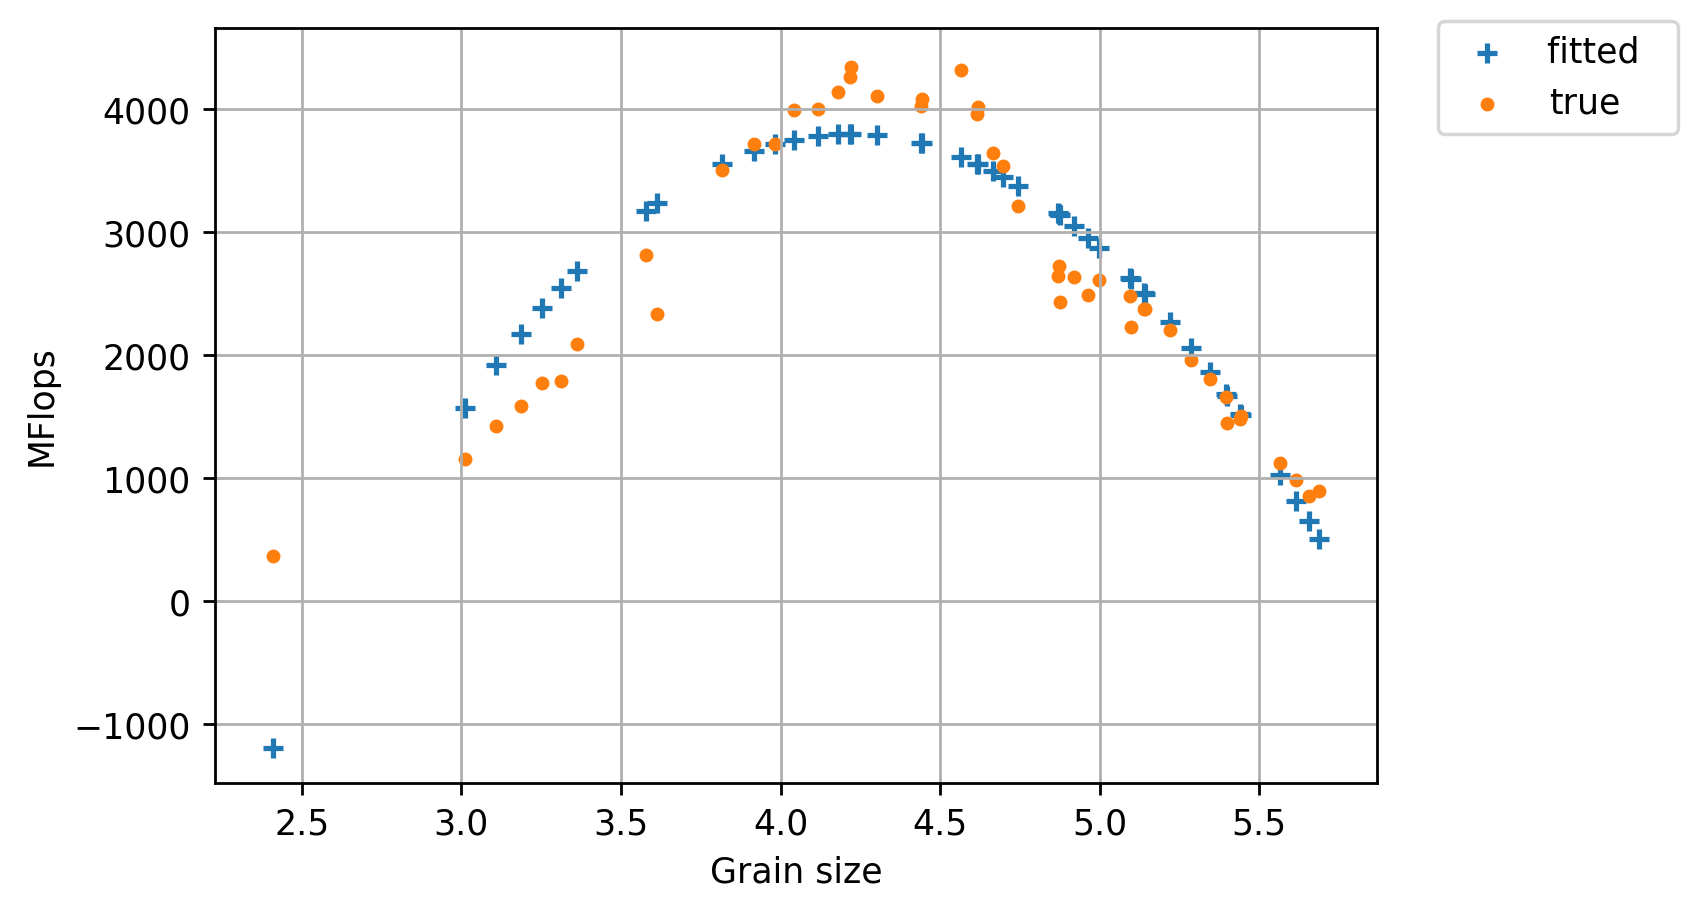
\includegraphics[scale=.3]{images/polyfit/fig_8_690.png}\label{fig10:h}}
			
			\caption{The results of fitting the throughput vs grain size data into a 2d polynomial for $DMATDMATADD$ benchmark for matrix size 690$\times$690 with different number of cores on the test data.}
			\label{fig10}
		\end{figure}
	\end{outline}
\end{frame}

%\begin{frame}{Method: Modeling Performance based on Grain Size}
%	\begin{outline}	
%		\begin{figure}[H]
%			\centering
%			\subfloat[1 core]{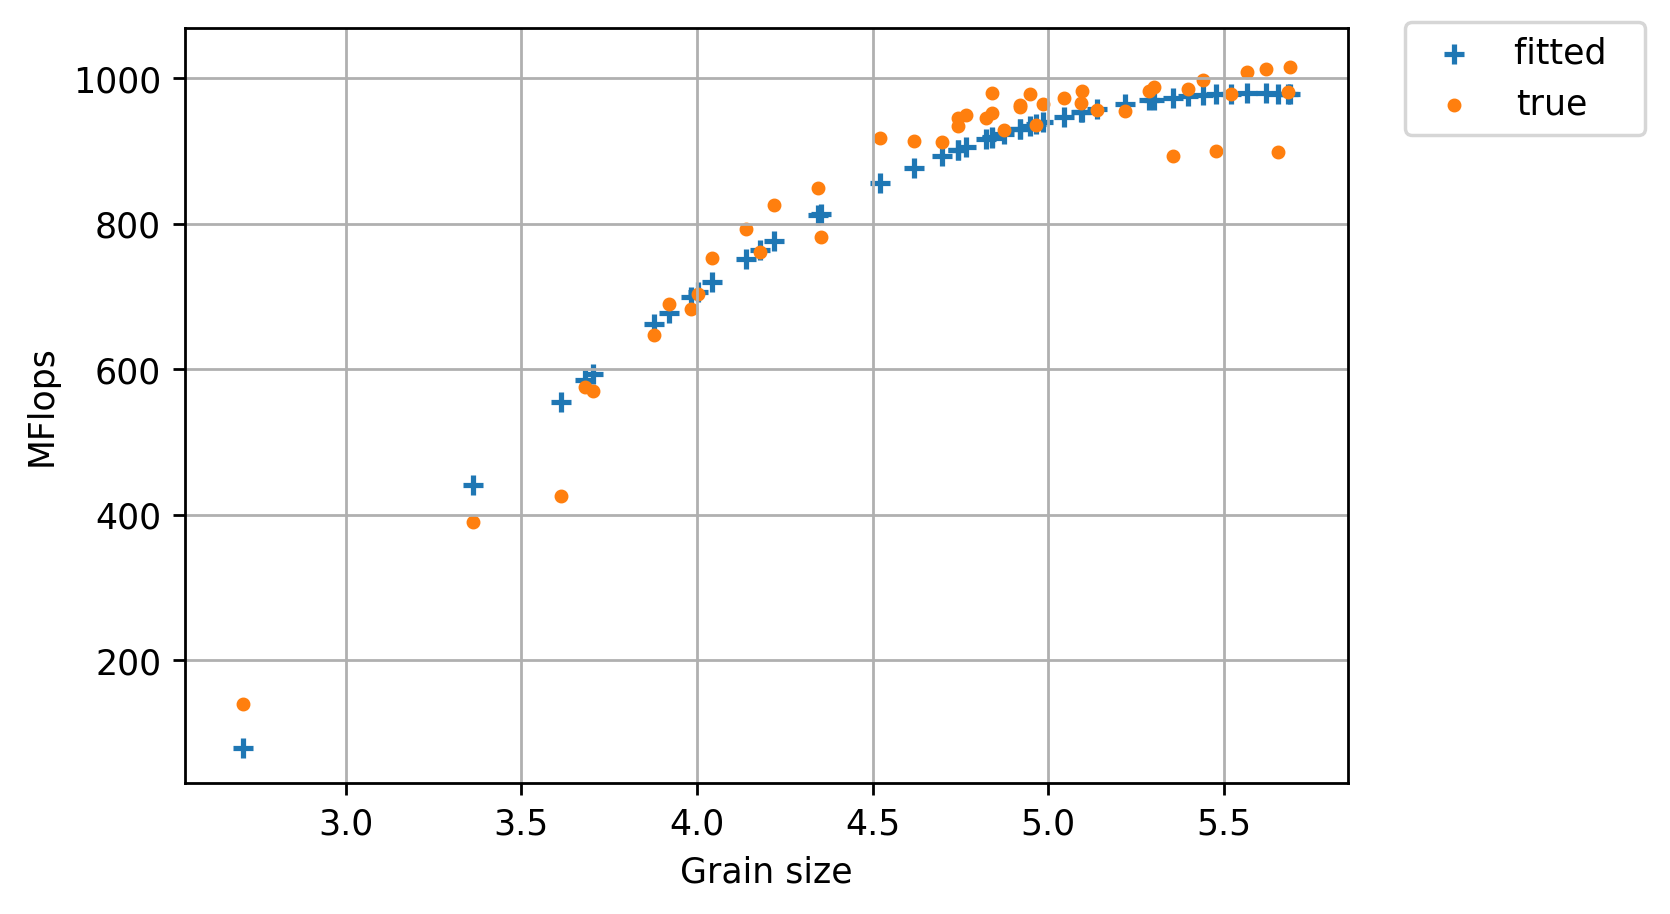
\includegraphics[scale=.15]{images/polyfit/fig_1_690.png}\label{fig40:a}}
%			\subfloat[2 cores]{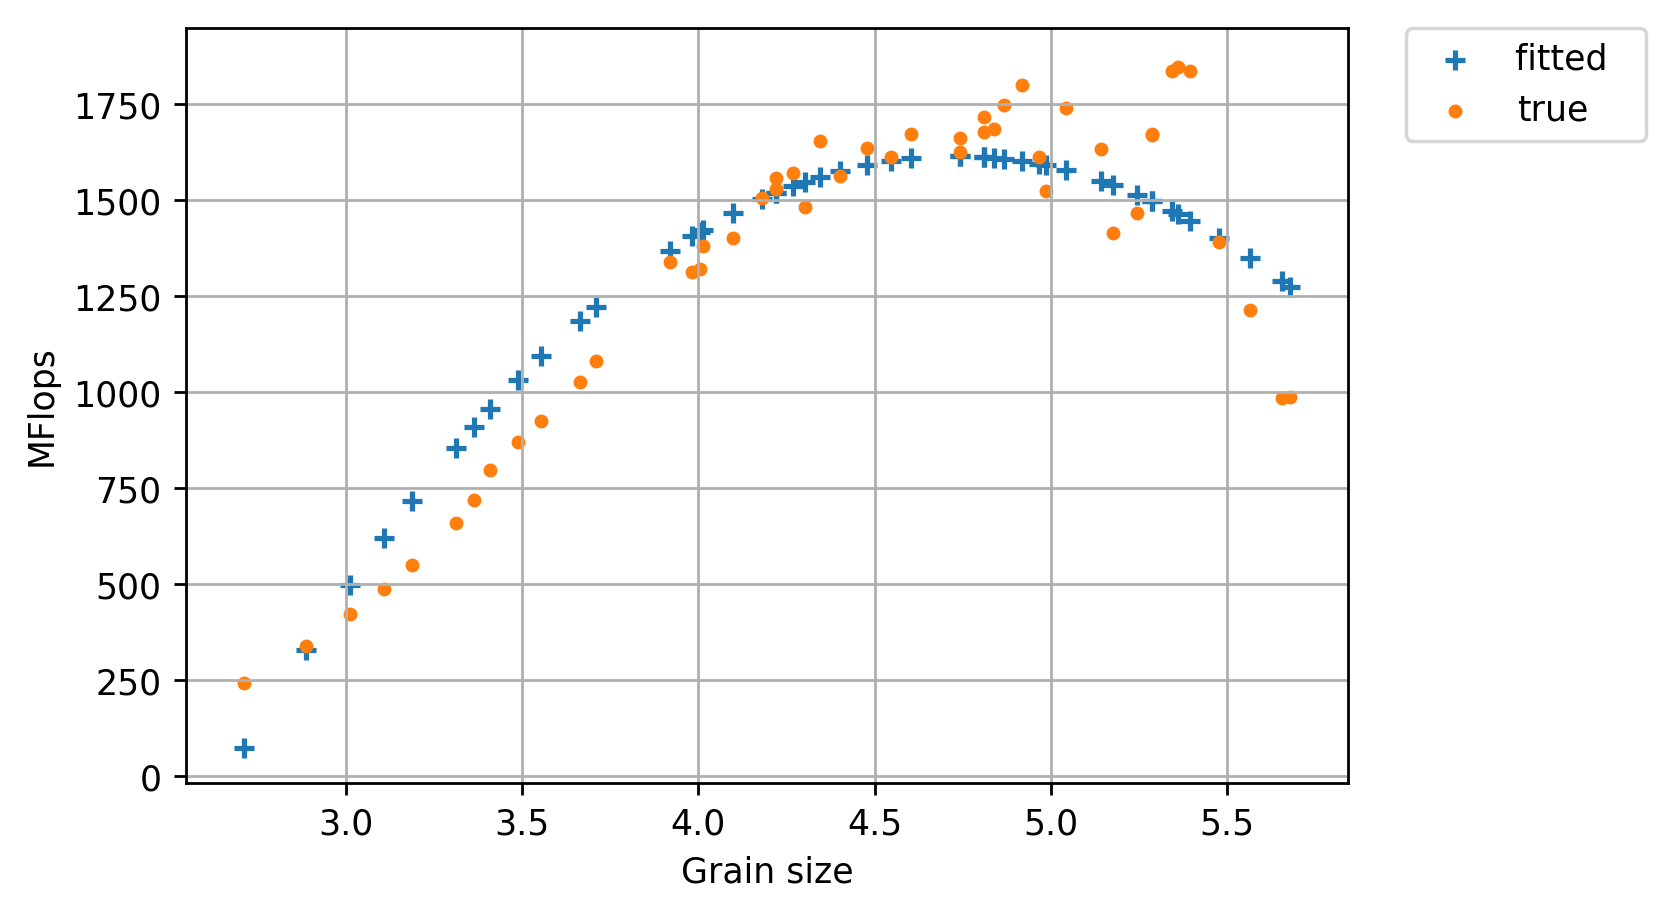
\includegraphics[scale=.15]{images/polyfit/fig_2_690.png}\label{fig40:b}}
%			\subfloat[3 cores]{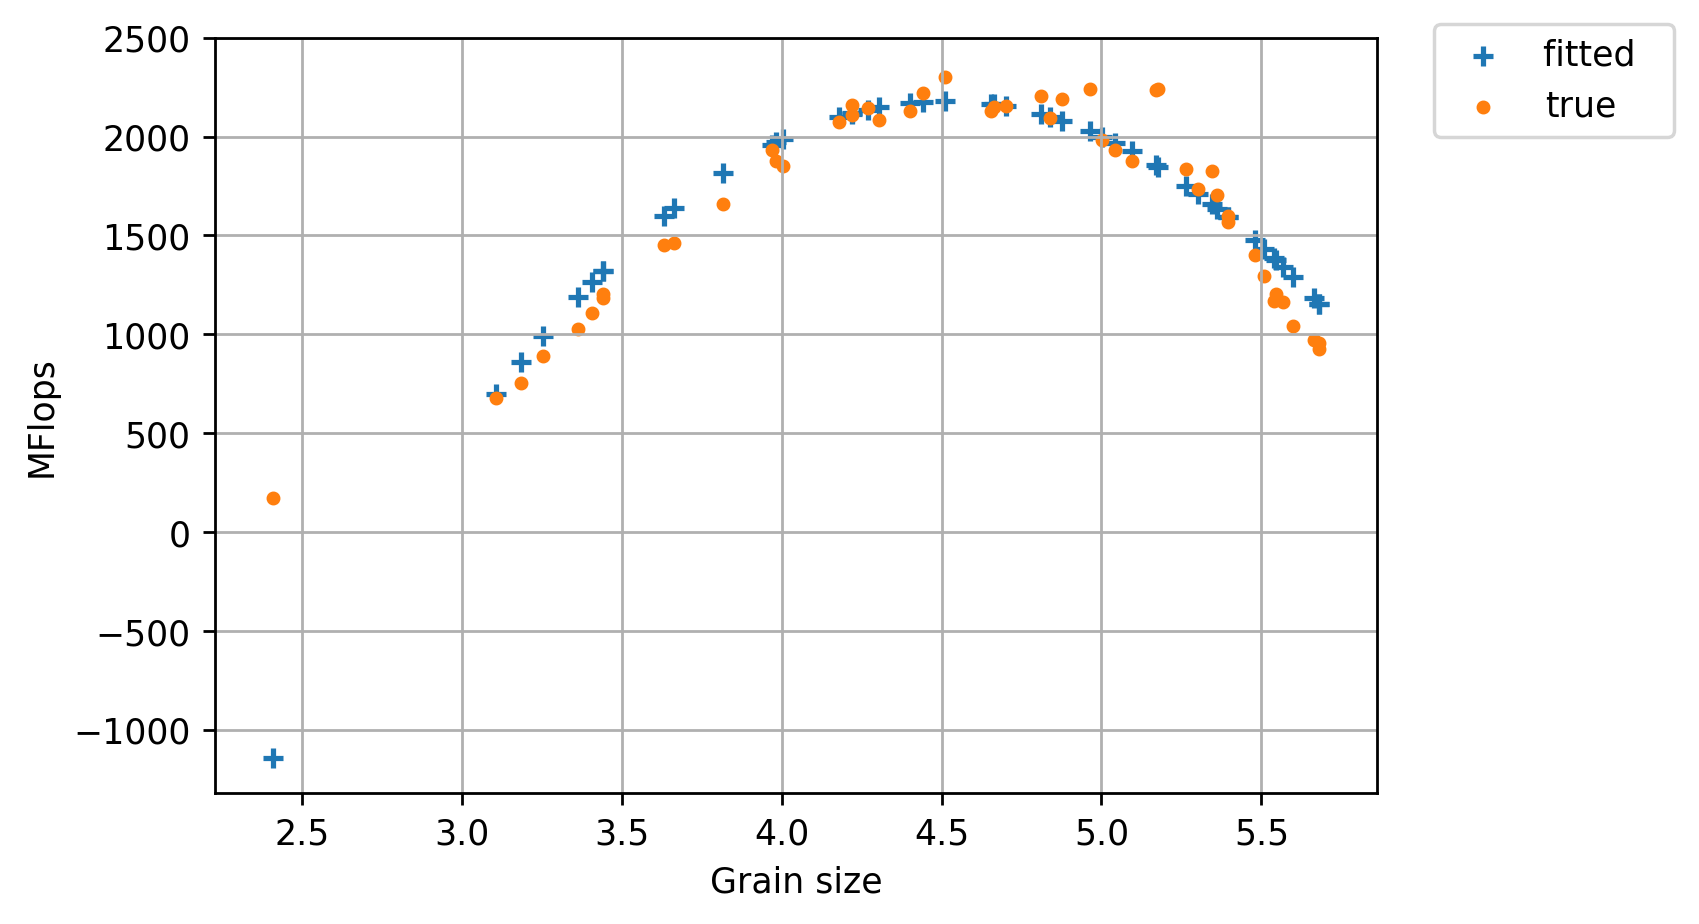
\includegraphics[scale=.15]{images/polyfit/fig_3_690.png}\label{fig40:c}}
%			\subfloat[4 cores]{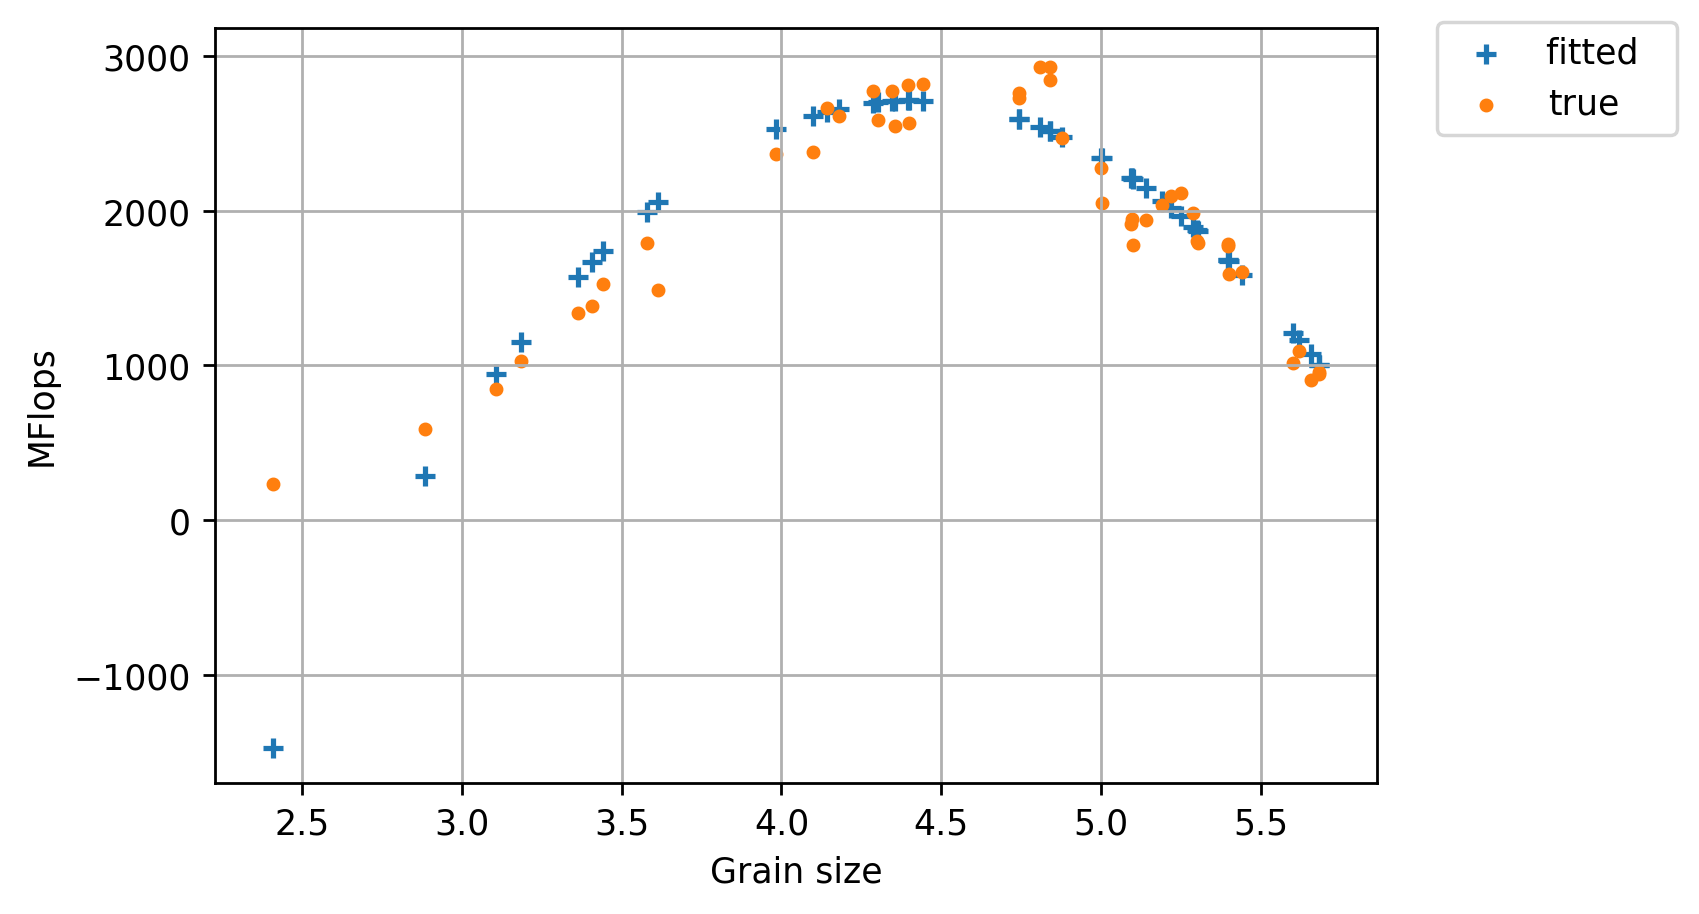
\includegraphics[scale=.15]{images/polyfit/fig_4_690.png}\label{fig40:d}}{\hfill}
%			\subfloat[5 cores]{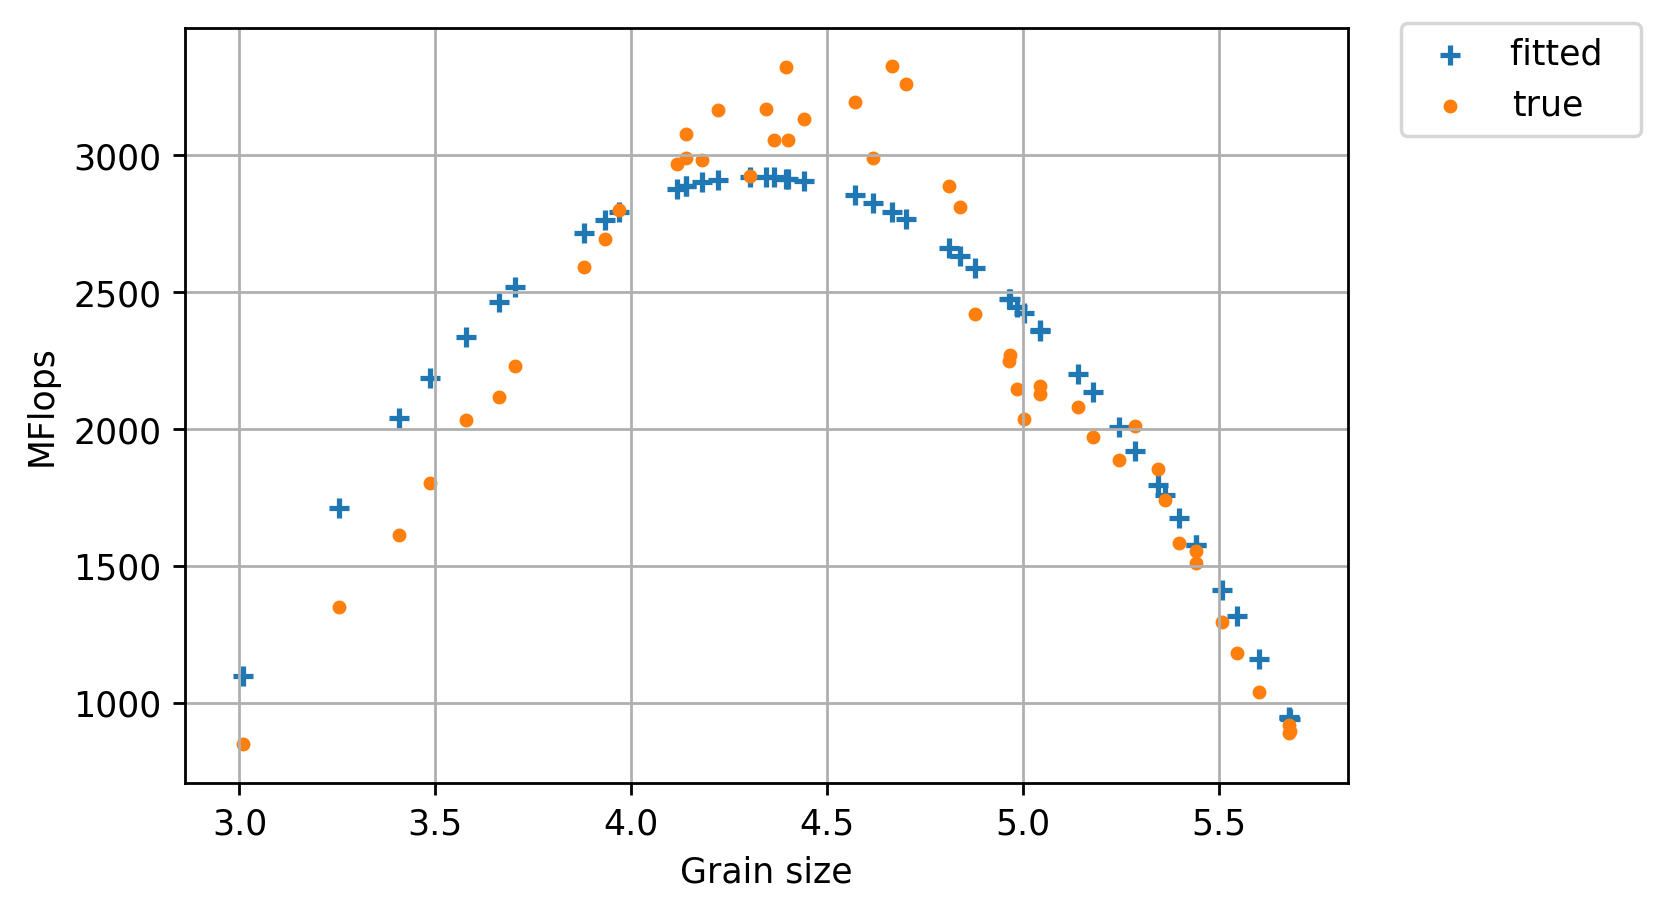
\includegraphics[scale=.15]{images/polyfit/fig_5_690.png}\label{fig40:e}}
%			\subfloat[6 cores]{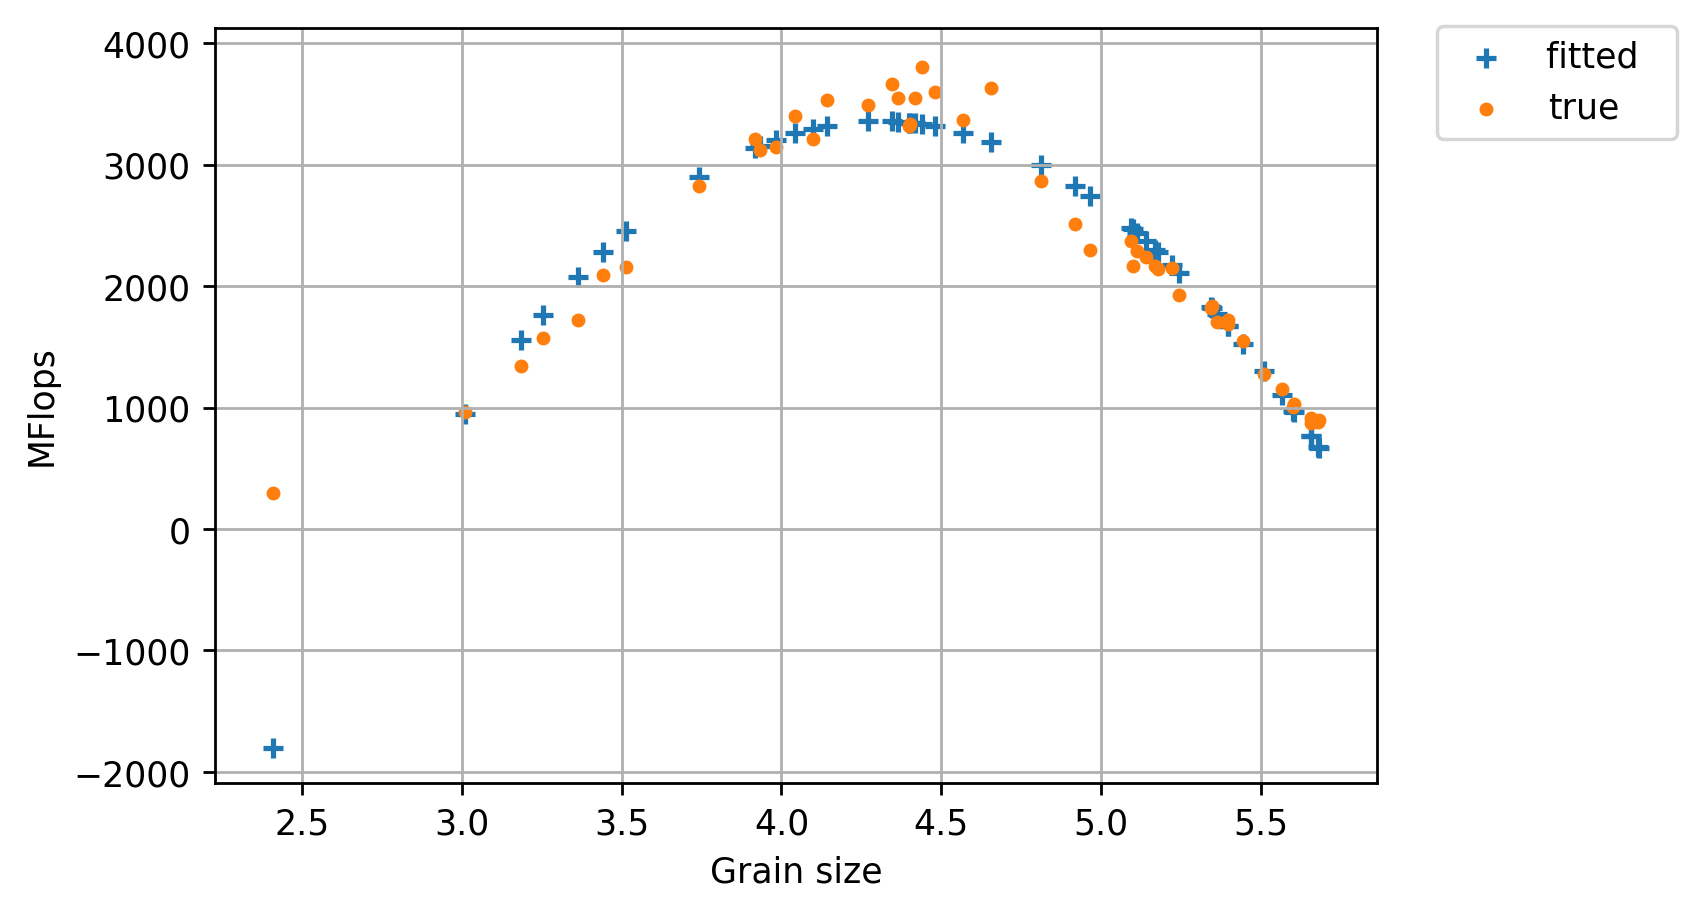
\includegraphics[scale=.15]{images/polyfit/fig_6_690.png}\label{fig40:f}}
%			\subfloat[7 cores]{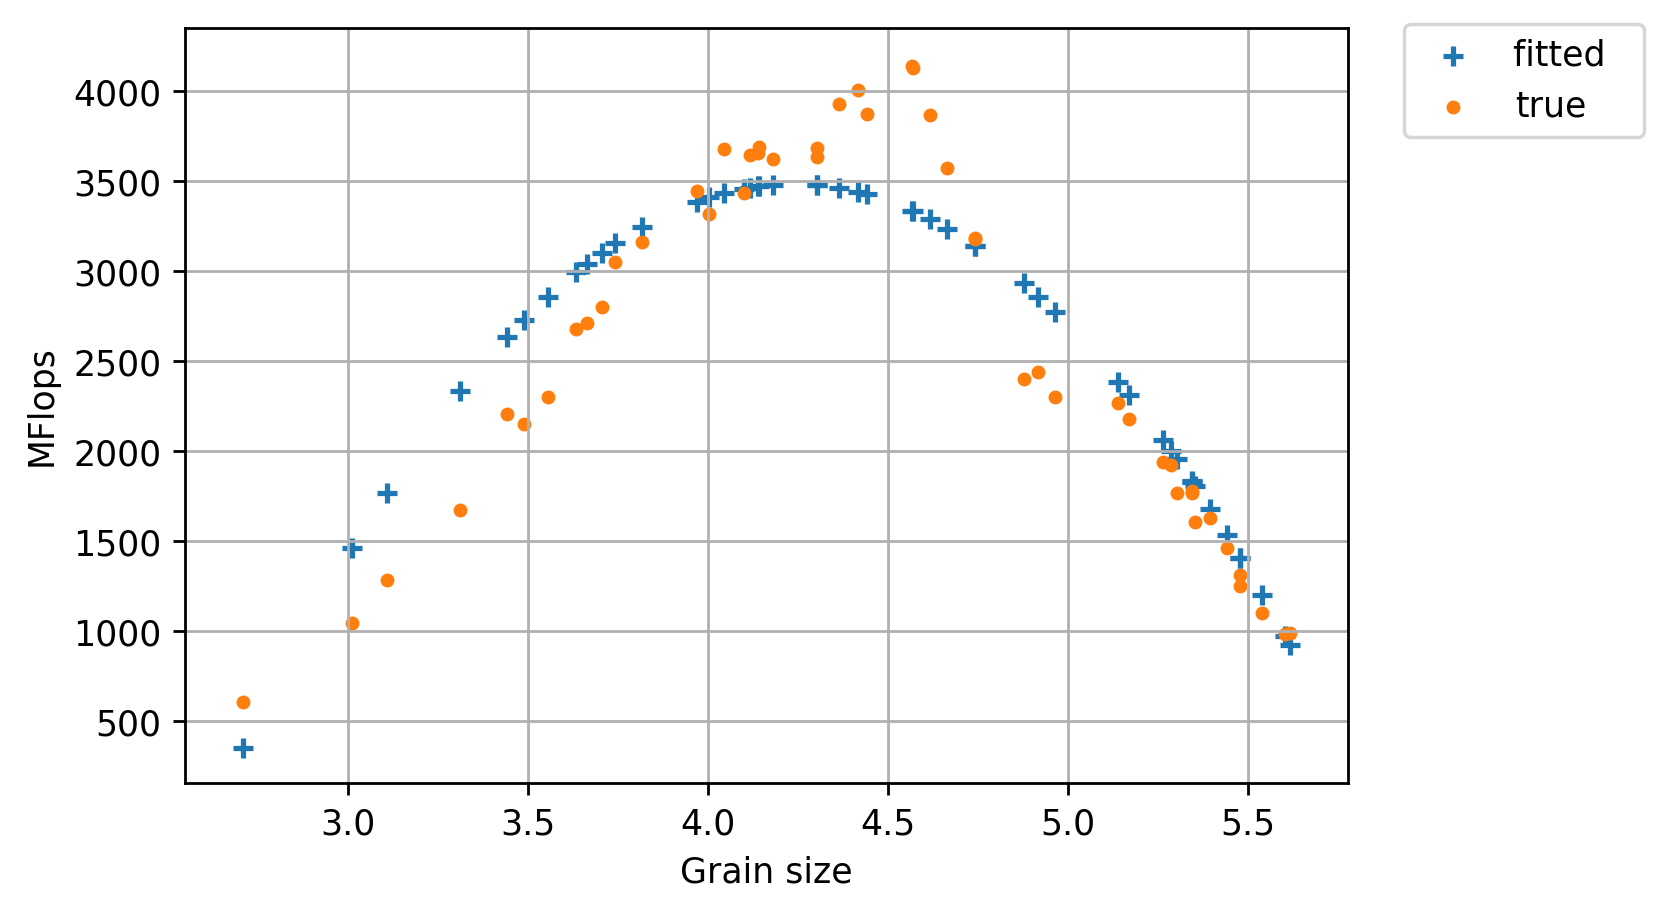
\includegraphics[scale=.15]{images/polyfit/fig_7_690.png}\label{fig40:g}}
%			\subfloat[8 cores]{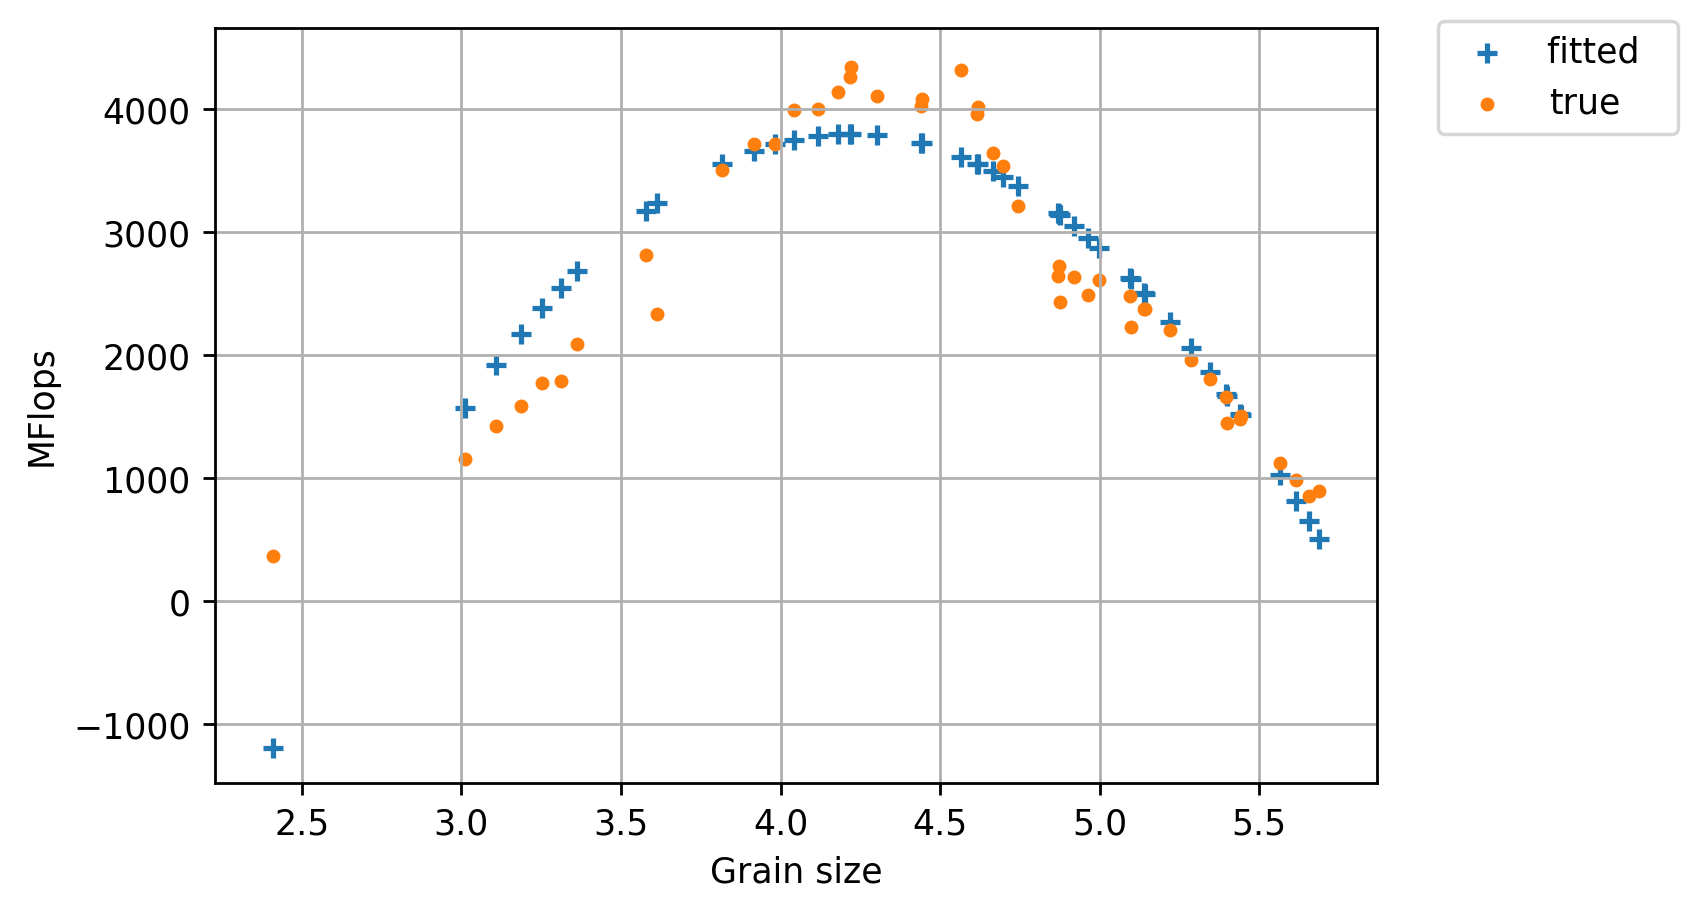
\includegraphics[scale=.15]{images/polyfit/fig_8_690.png}\label{fig40:h}}
%			
%			\caption{The results of fitting the throughput vs grain size data into a 2d polynomial for $DMATDMATADD$ benchmark for matrix size 1587$\times$1587 with different number of cores on the test data.}
%			\label{fig10}
%		\end{figure}
%	\end{outline}
%\end{frame}



\begin{frame}{Method: Modeling Performance based on Grain Size}
	\begin{outline}	
		$$R\textunderscore{squared} = 1-\frac{{\frac{1}{n}\sum_{i=1}^{n}{(t_i-p_i)}^2}}{Var(t)}$$
%		$$n \text{ is the number of samples}$$
		\begin{figure}[H]
			\centering
			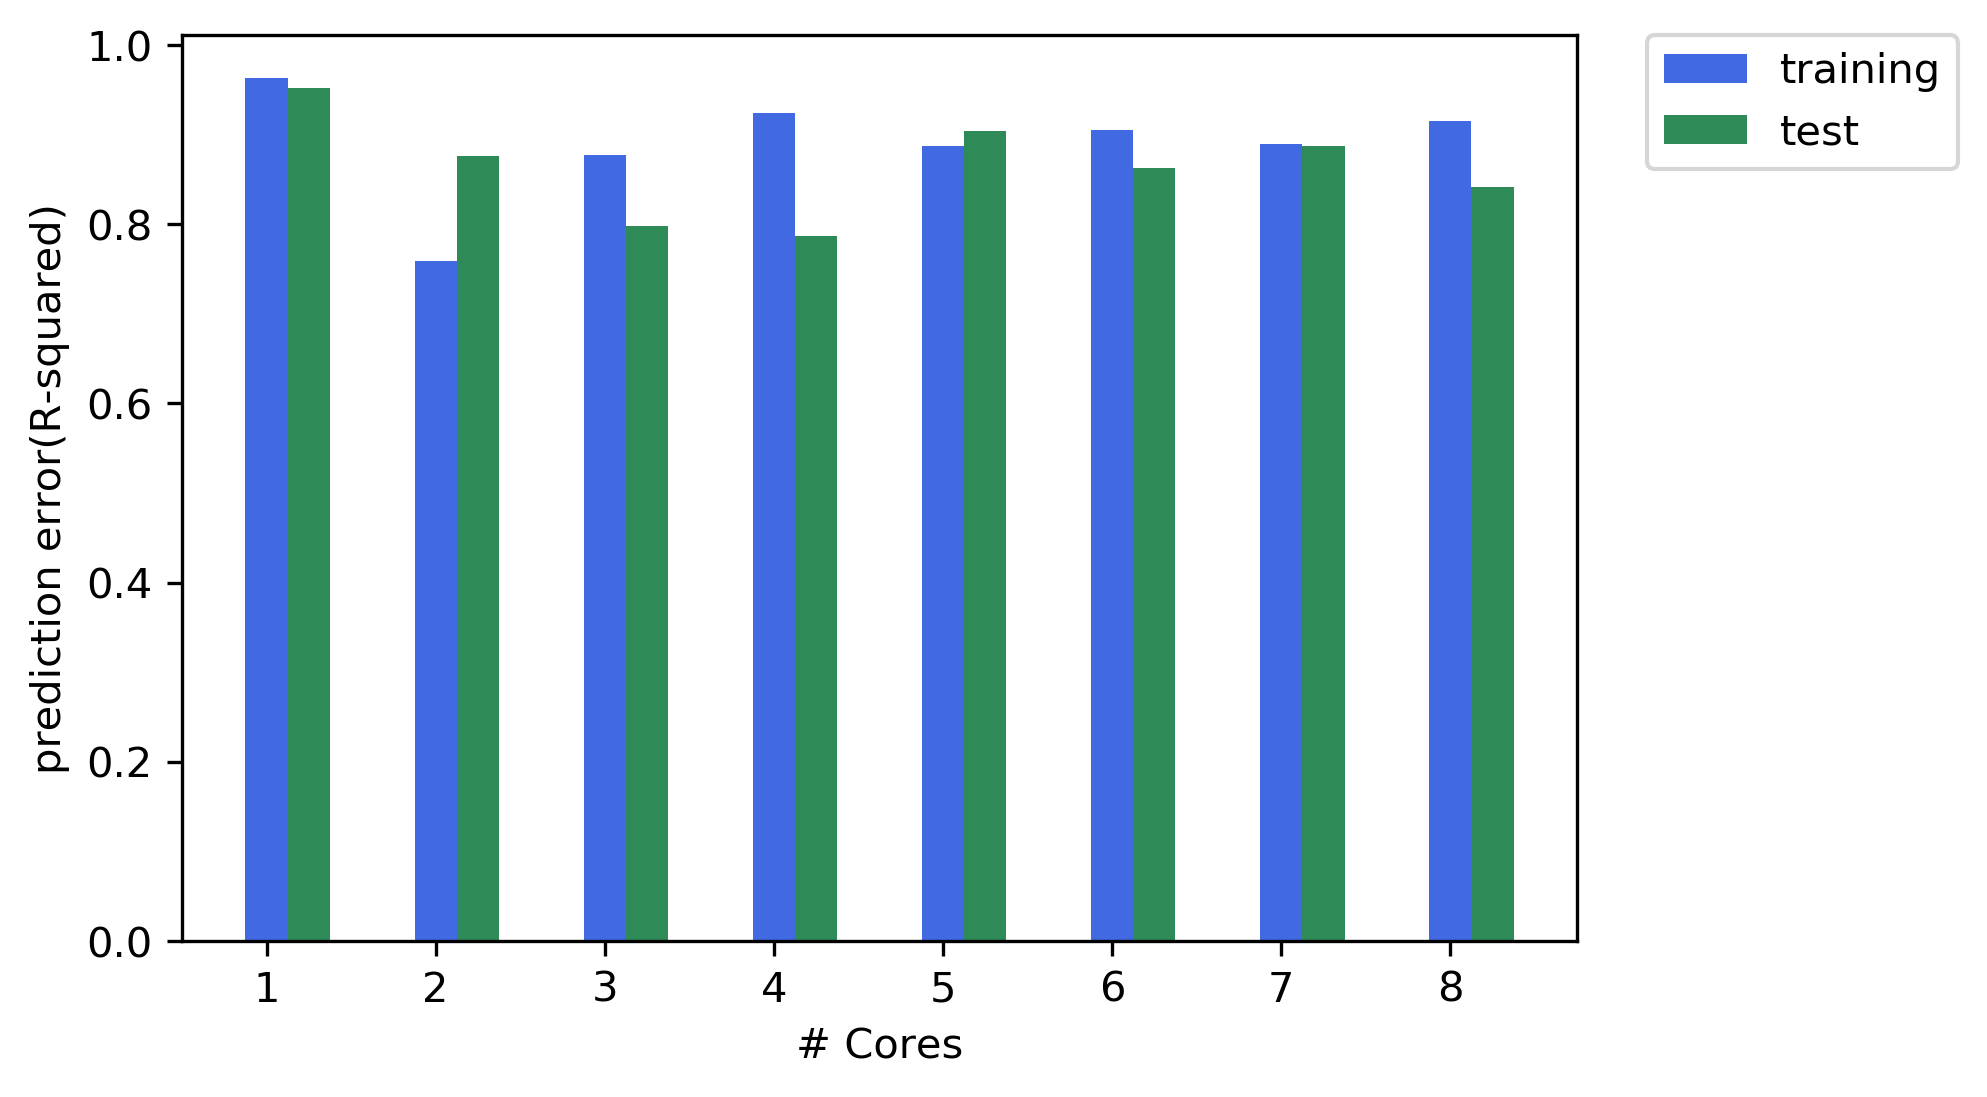
\includegraphics[scale=.5]{images/polyfit/error_690_r2.png}
			\caption{The training and test error for fitting data obtained from the $DMATDMATADD$ benchmark for matrix size $690\times690$ against different number of cores cores.}	
			\label{fig33}
		\end{figure}
	\end{outline}
\end{frame}

\begin{frame}{Method: Modeling Performance based on Grain Size}
	\begin{outline}	
		\begin{figure}
		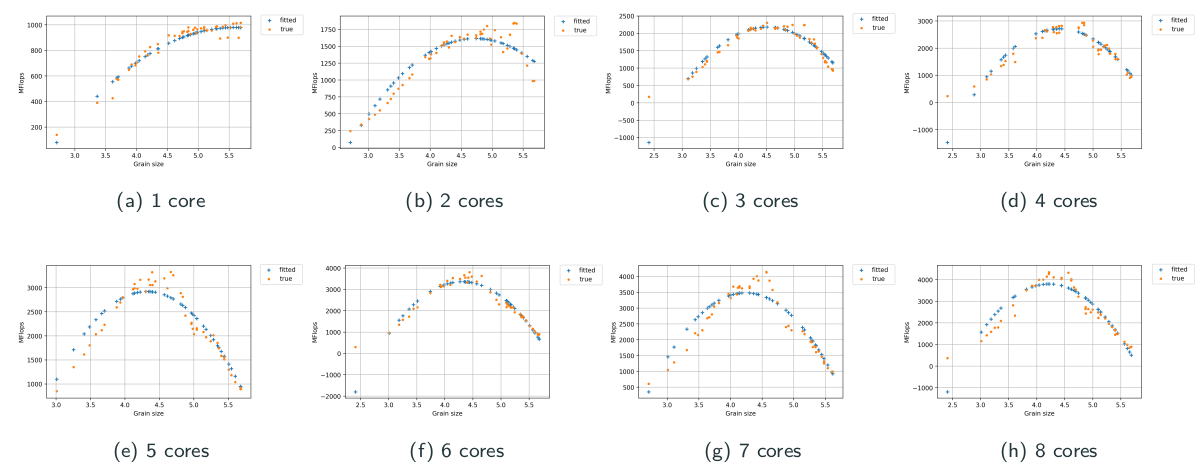
\includegraphics[scale=.15]{images/polyfit/model_1_8.png}
		\end{figure}

		\1We have developed a model for each number of cores:1, 2,.., 8 $P=ag^2+bg+c$\\ 
		\pause
		\1Can we somehow integrate number of cores into the model?
	\end{outline}
\end{frame}

\begin{frame}{Method: Modeling Performance based on Grain Size}
	\begin{outline}	
		\1For $P=ag^2+bg+c$, how do $a$, $b$, and $c$ change with the number of cores?		\\
		\begin{figure}[H]
			\centering
			{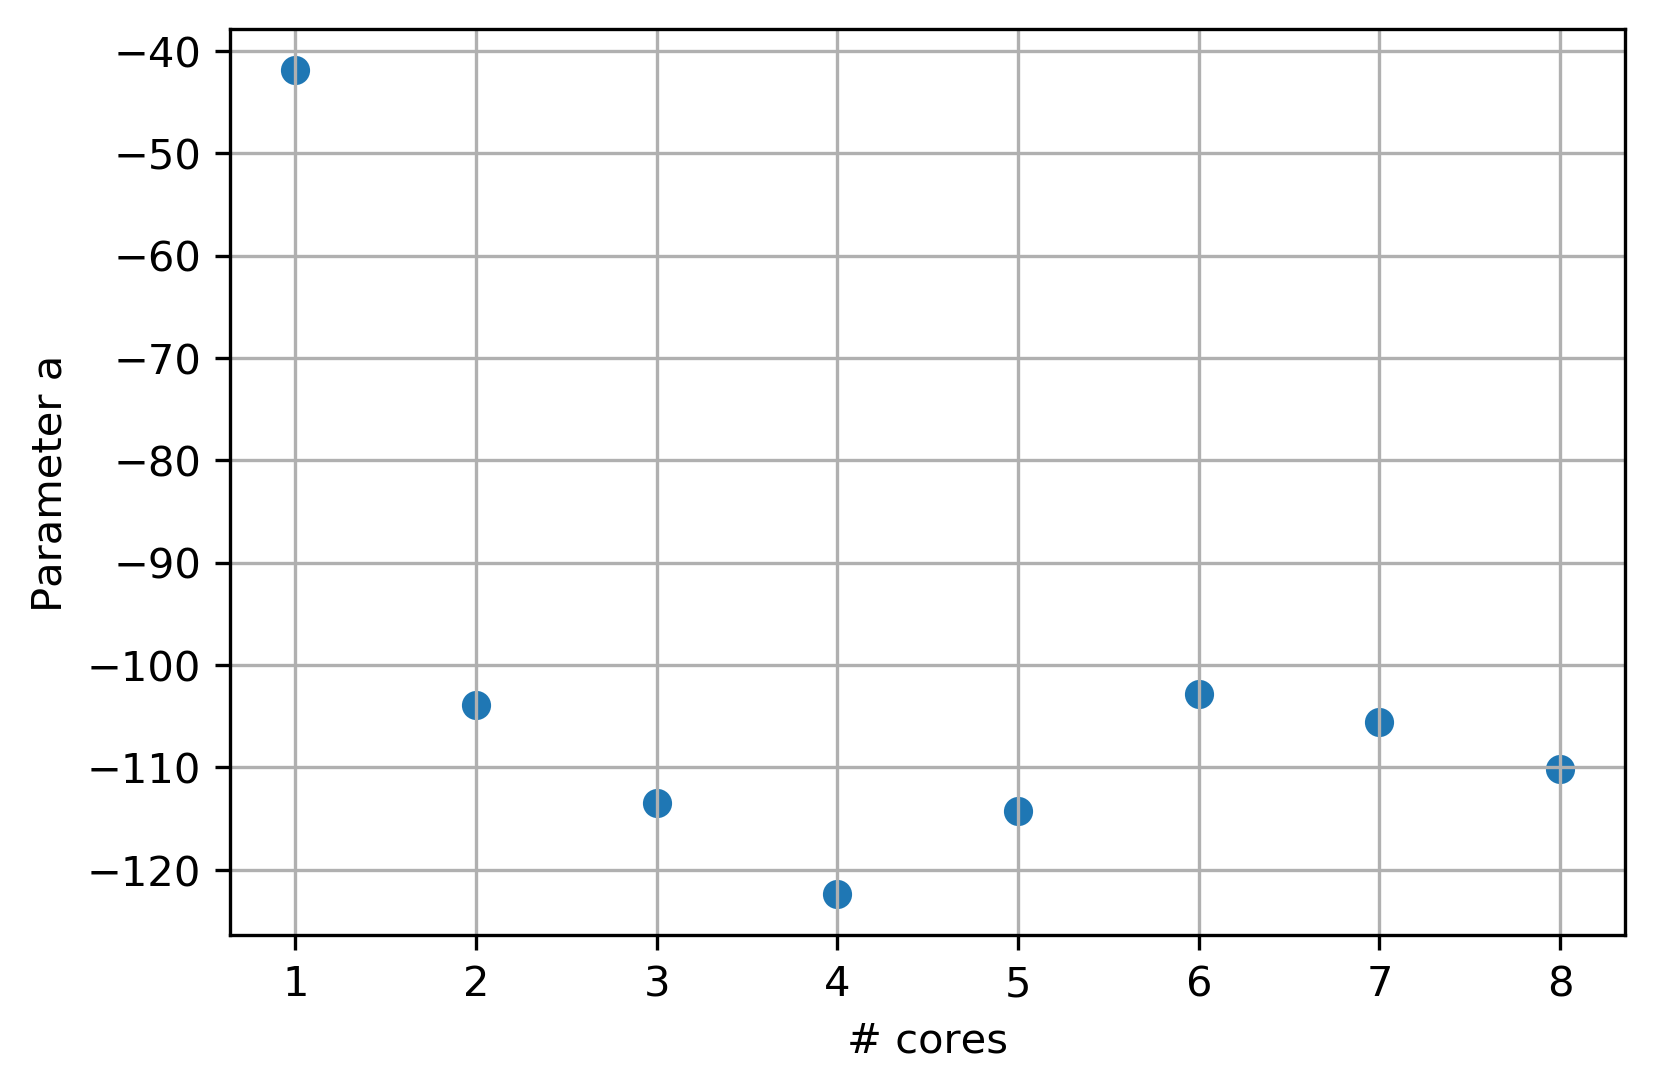
\includegraphics[scale=.33]{images/polyfit/fig_1587_params_0before_fit.png}\label{fig31:a}}
			{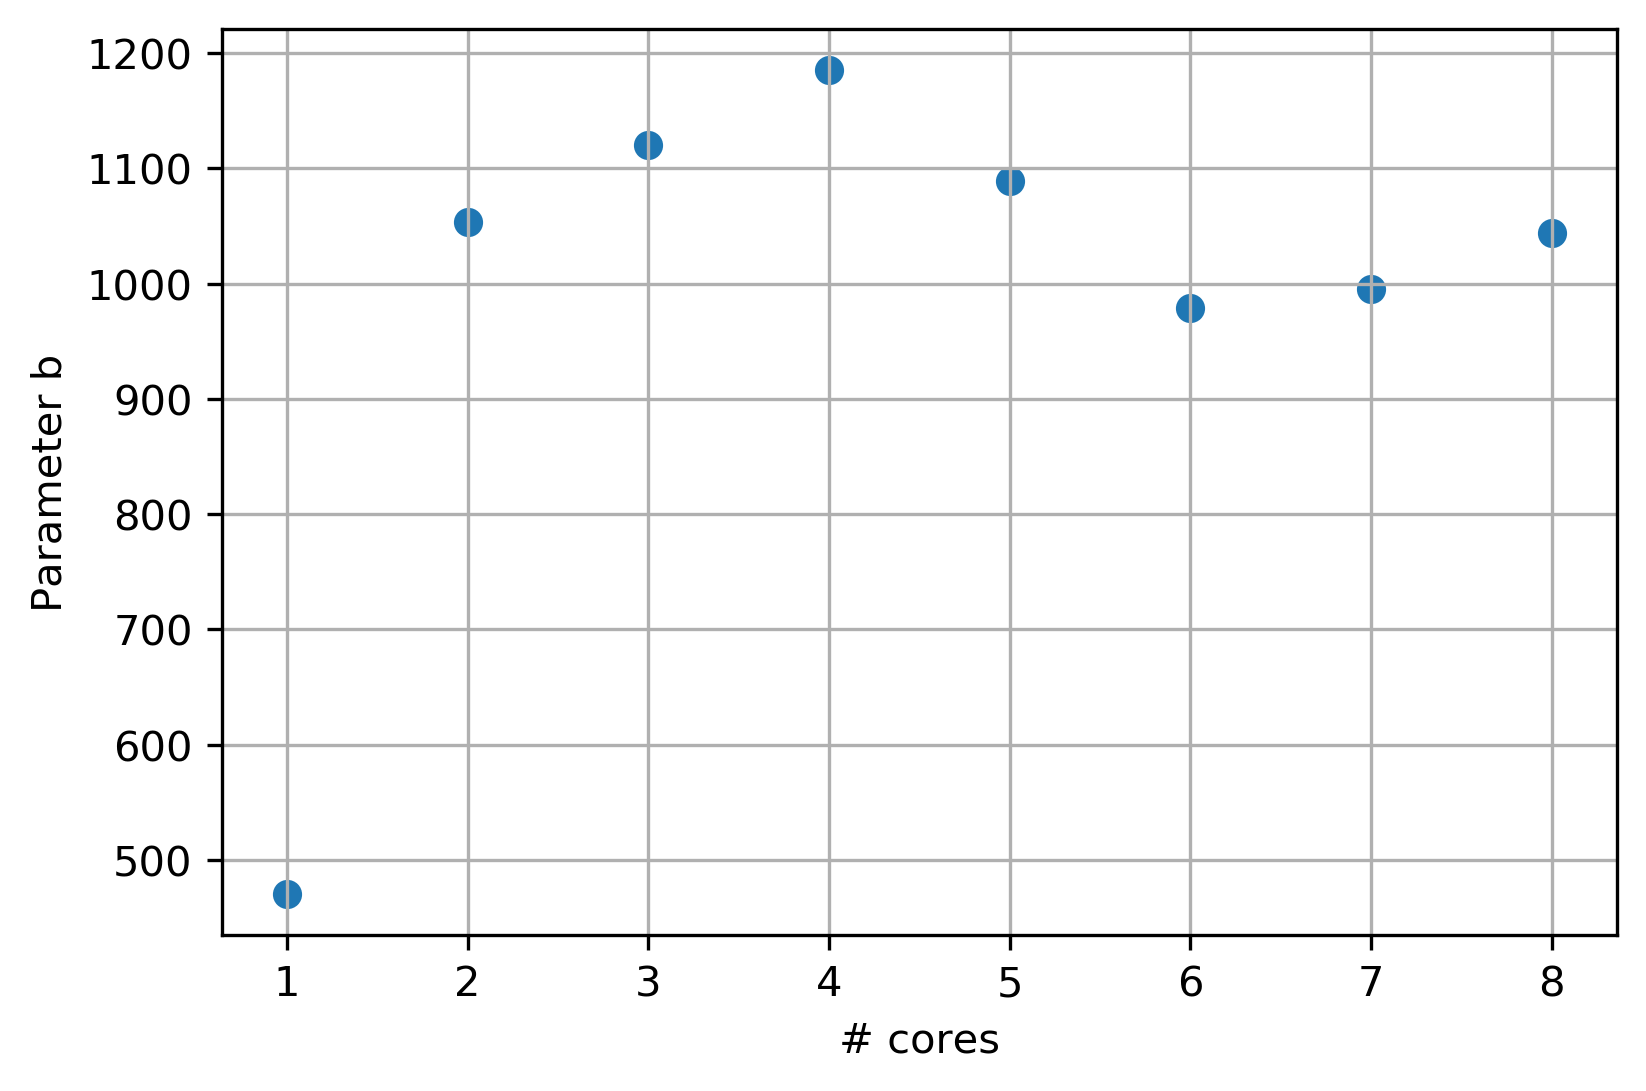
\includegraphics[scale=.33]{images/polyfit/fig_1587_params_1before_fit.png}\label{fig31:b}}
			{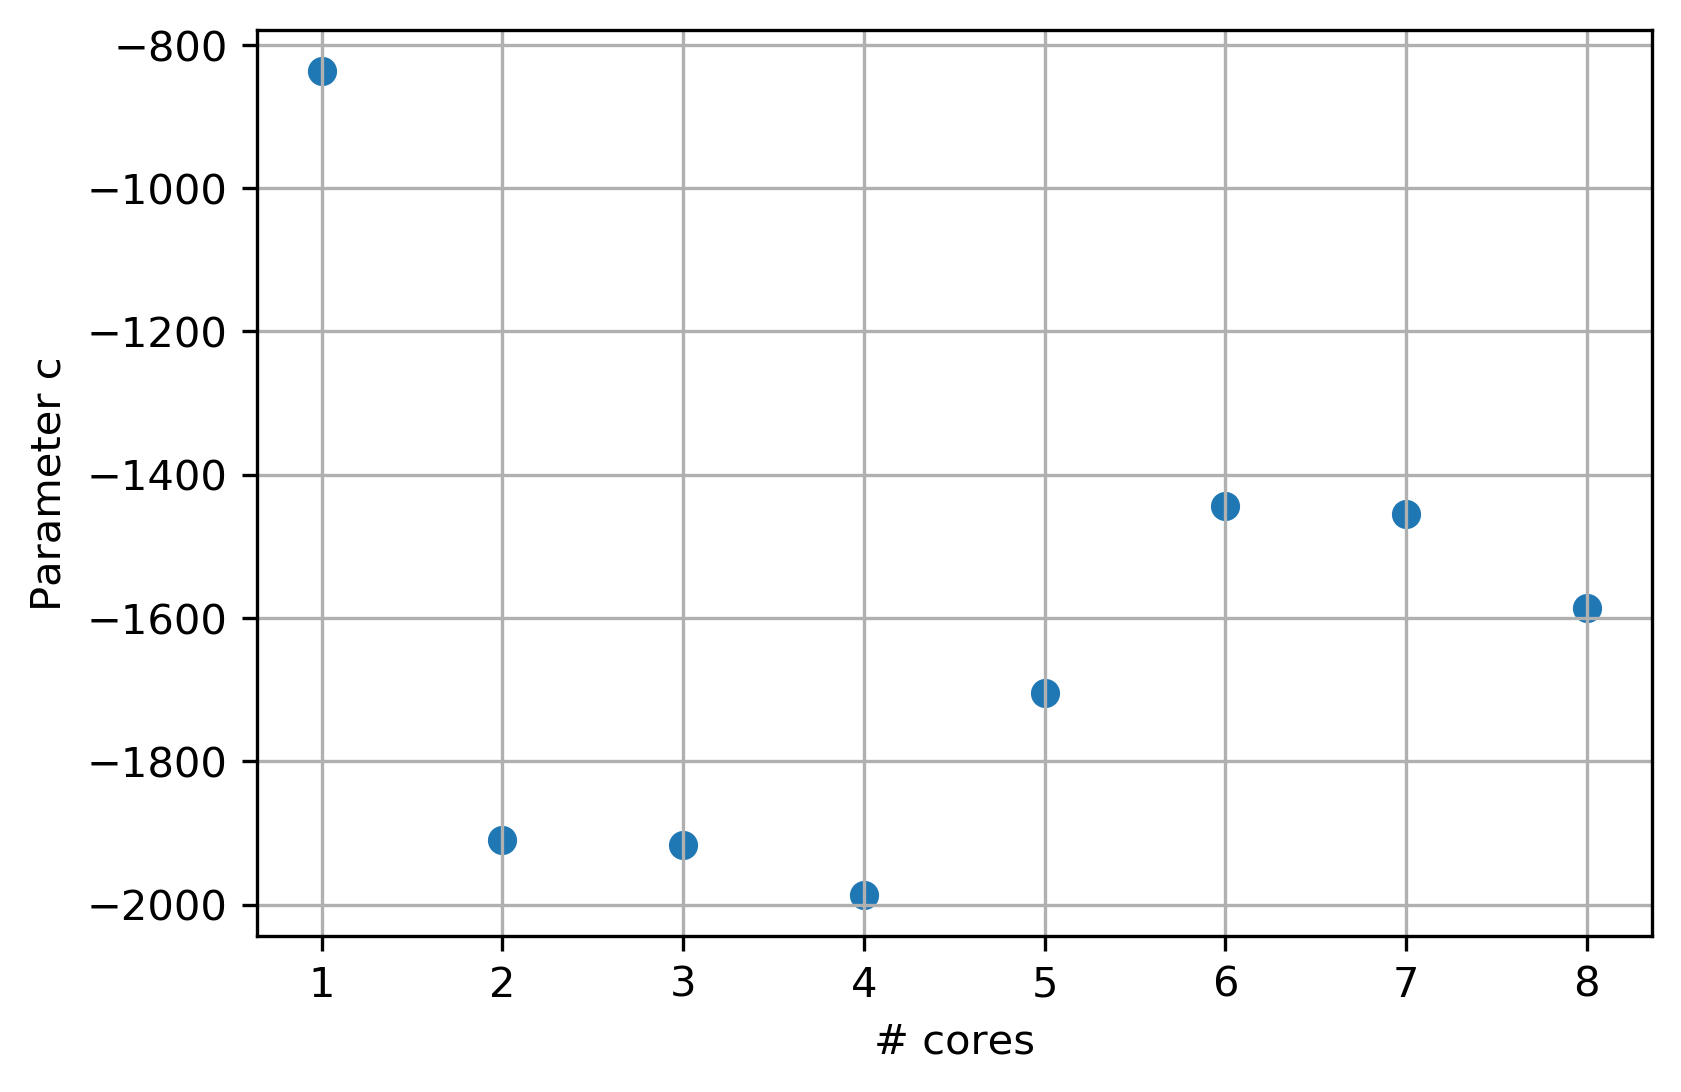
\includegraphics[scale=.33]{images/polyfit/fig_1587_params_2before_fit.png}\label{fig31:c}}
			\caption{The parameters of the polynomial fit from the $DMATDMATADD$ benchmark for matrix size $1587\times1587$ against different number of cores.}	
			\label{fig31}
		\end{figure}
	\end{outline}
\end{frame}

\begin{frame}{Method: Modeling Performance based on Grain Size}
	\begin{outline}			
		\1Model the relationship with a 3rd degree polynomial
		$$a=a_0N^3+a_1N^2+a_2N+a_3
		,\:\:\:\:\:b=b_0N^3+b_1N^2+b_2N+b_3,$$ $$c=c_0N^3+c_1N^2+c_2N+c_3$$
		\begin{figure}[H]
			\centering
			{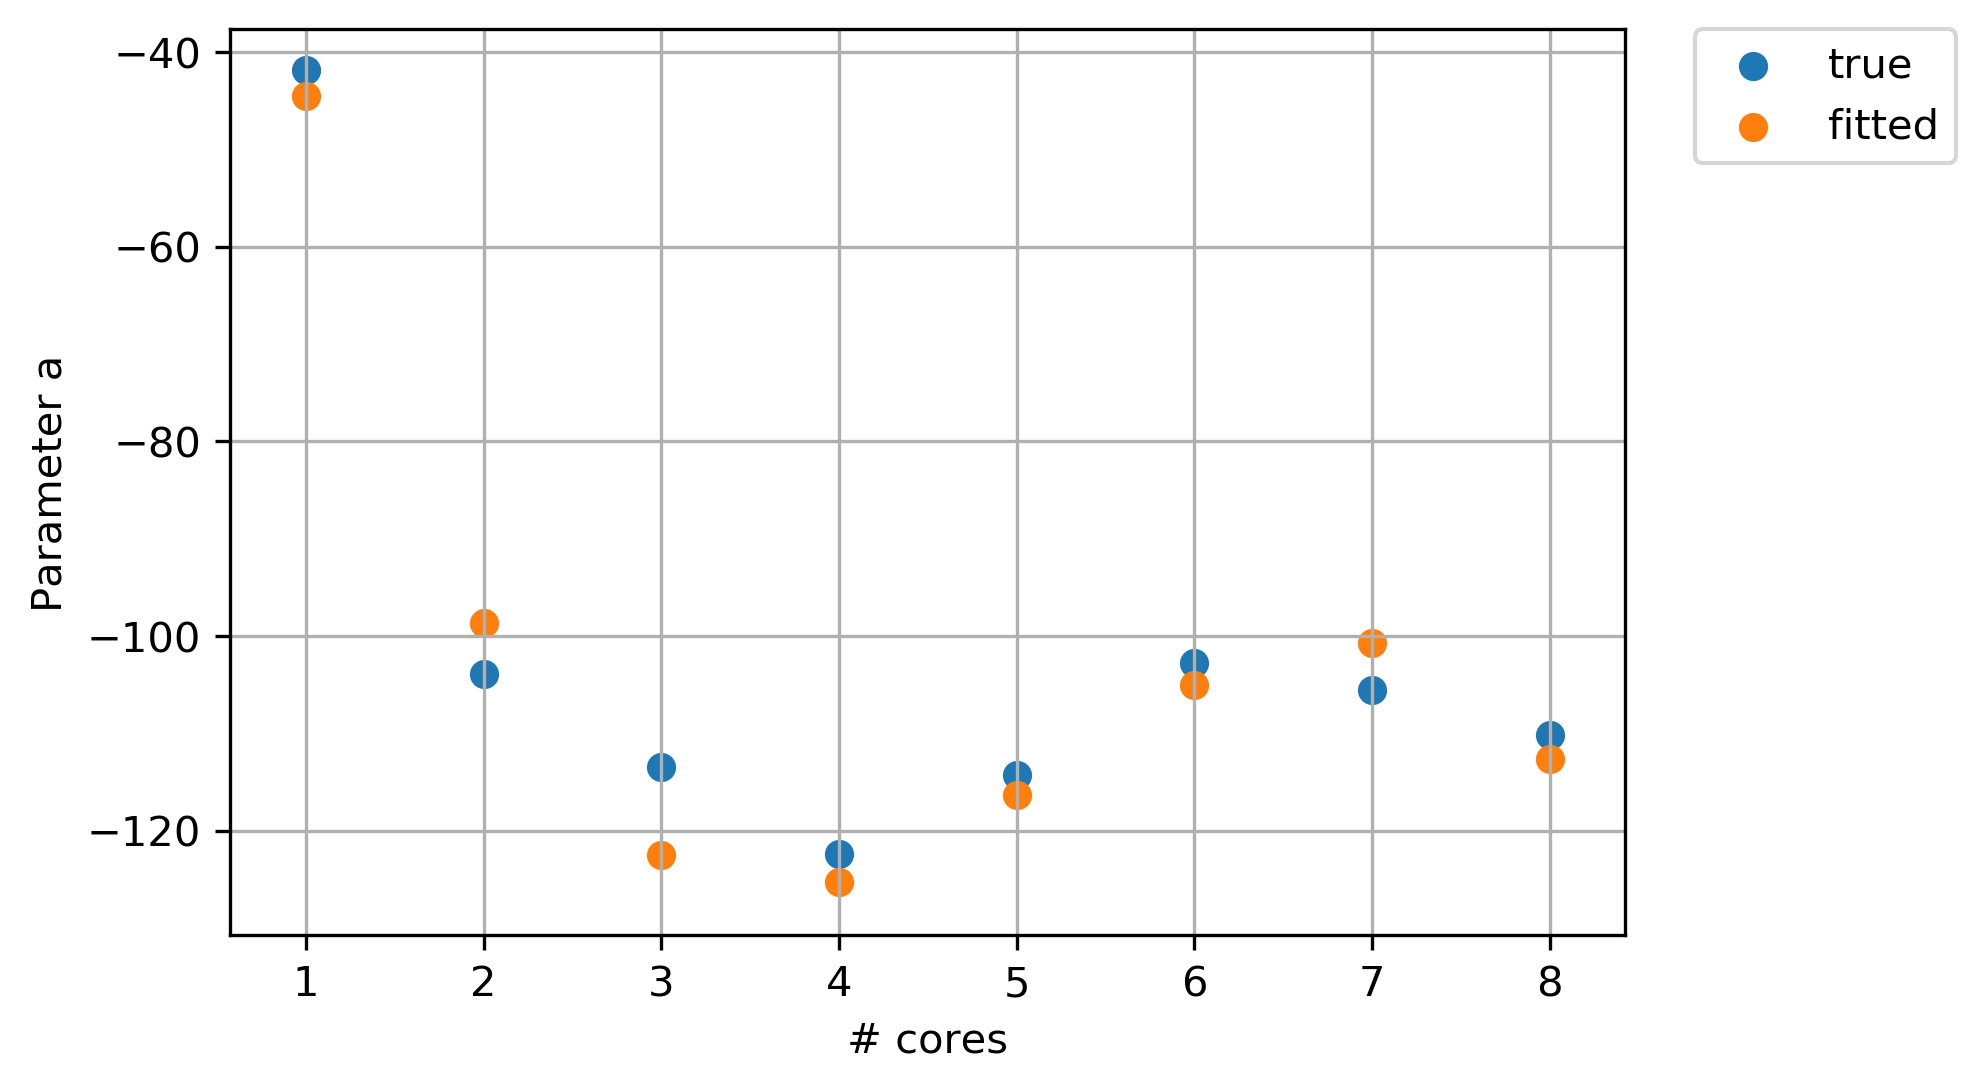
\includegraphics[scale=.25]{images/polyfit/fig_690_params_0.png}\label{fig15:a}}
			{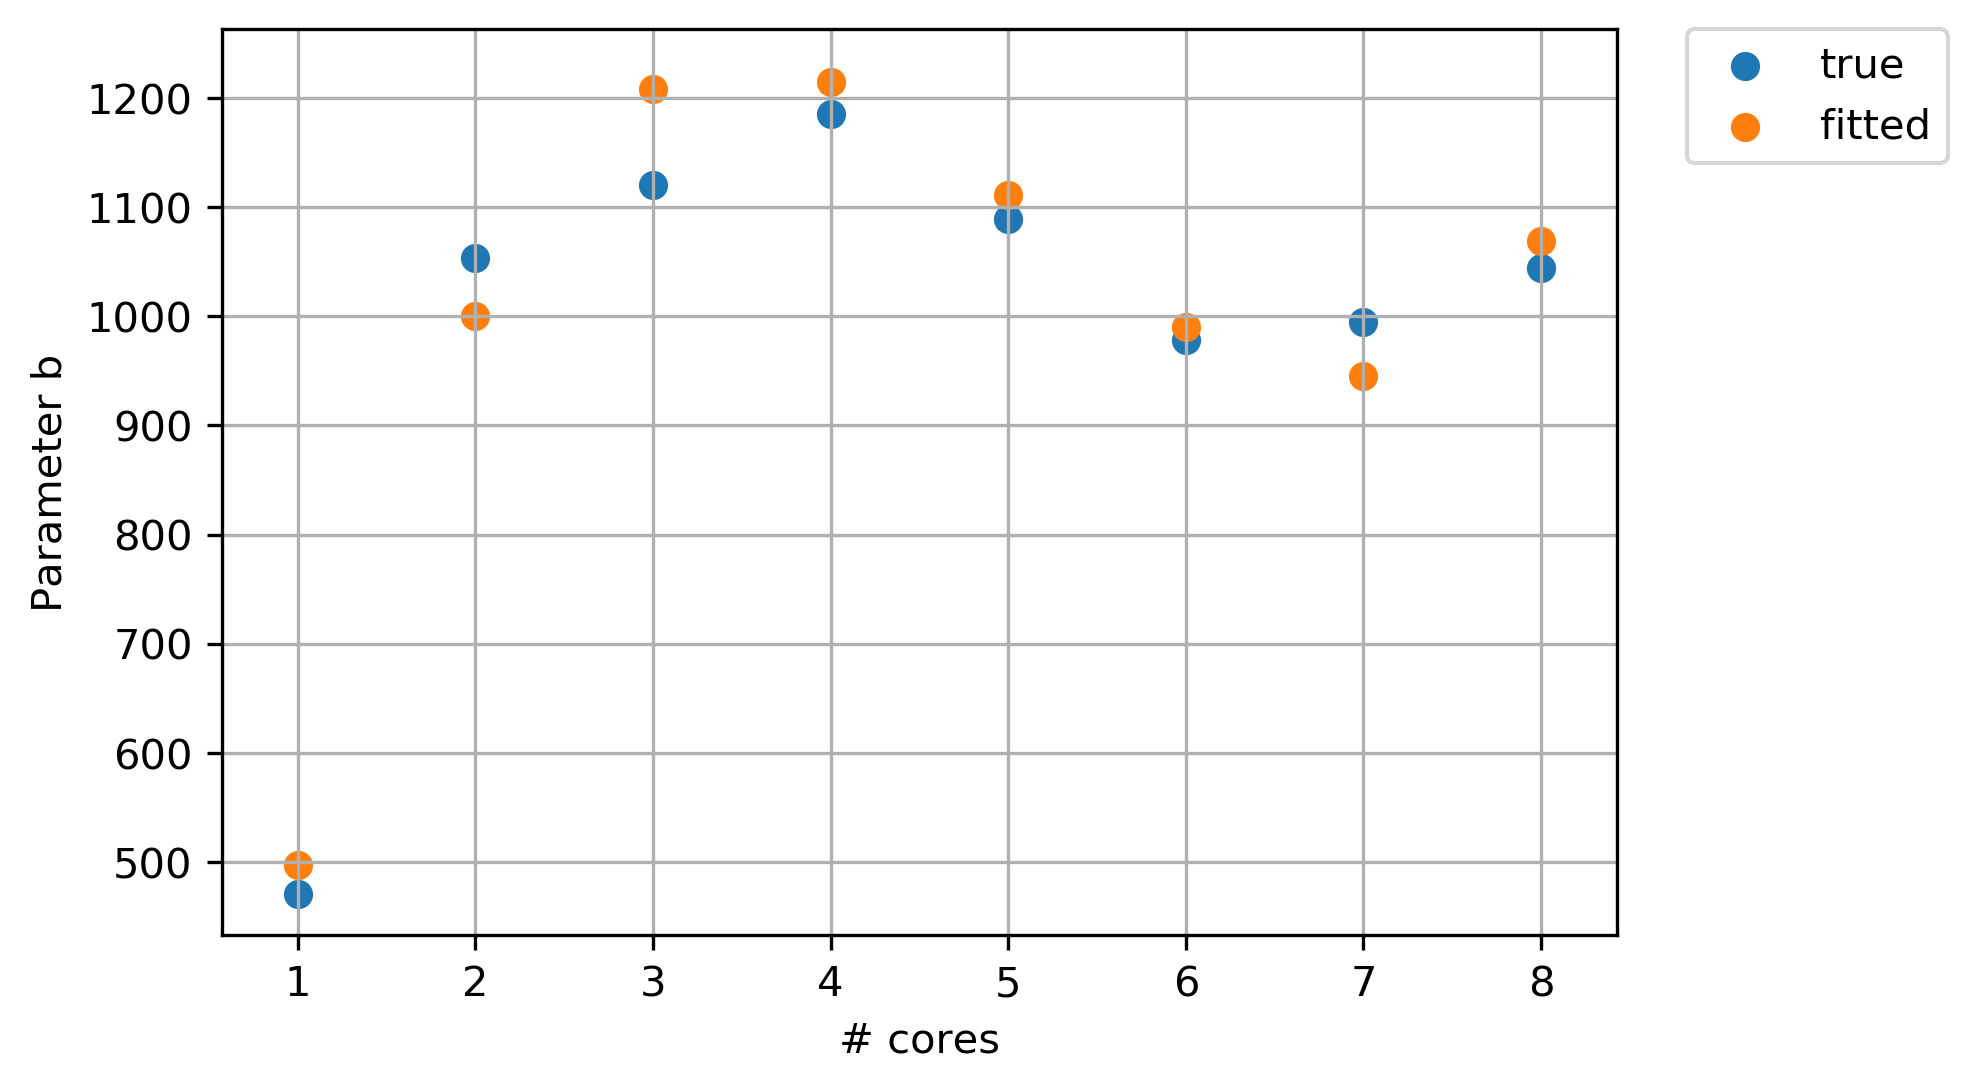
\includegraphics[scale=.25]{images/polyfit/fig_690_params_1.png}\label{fig15:b}}
			{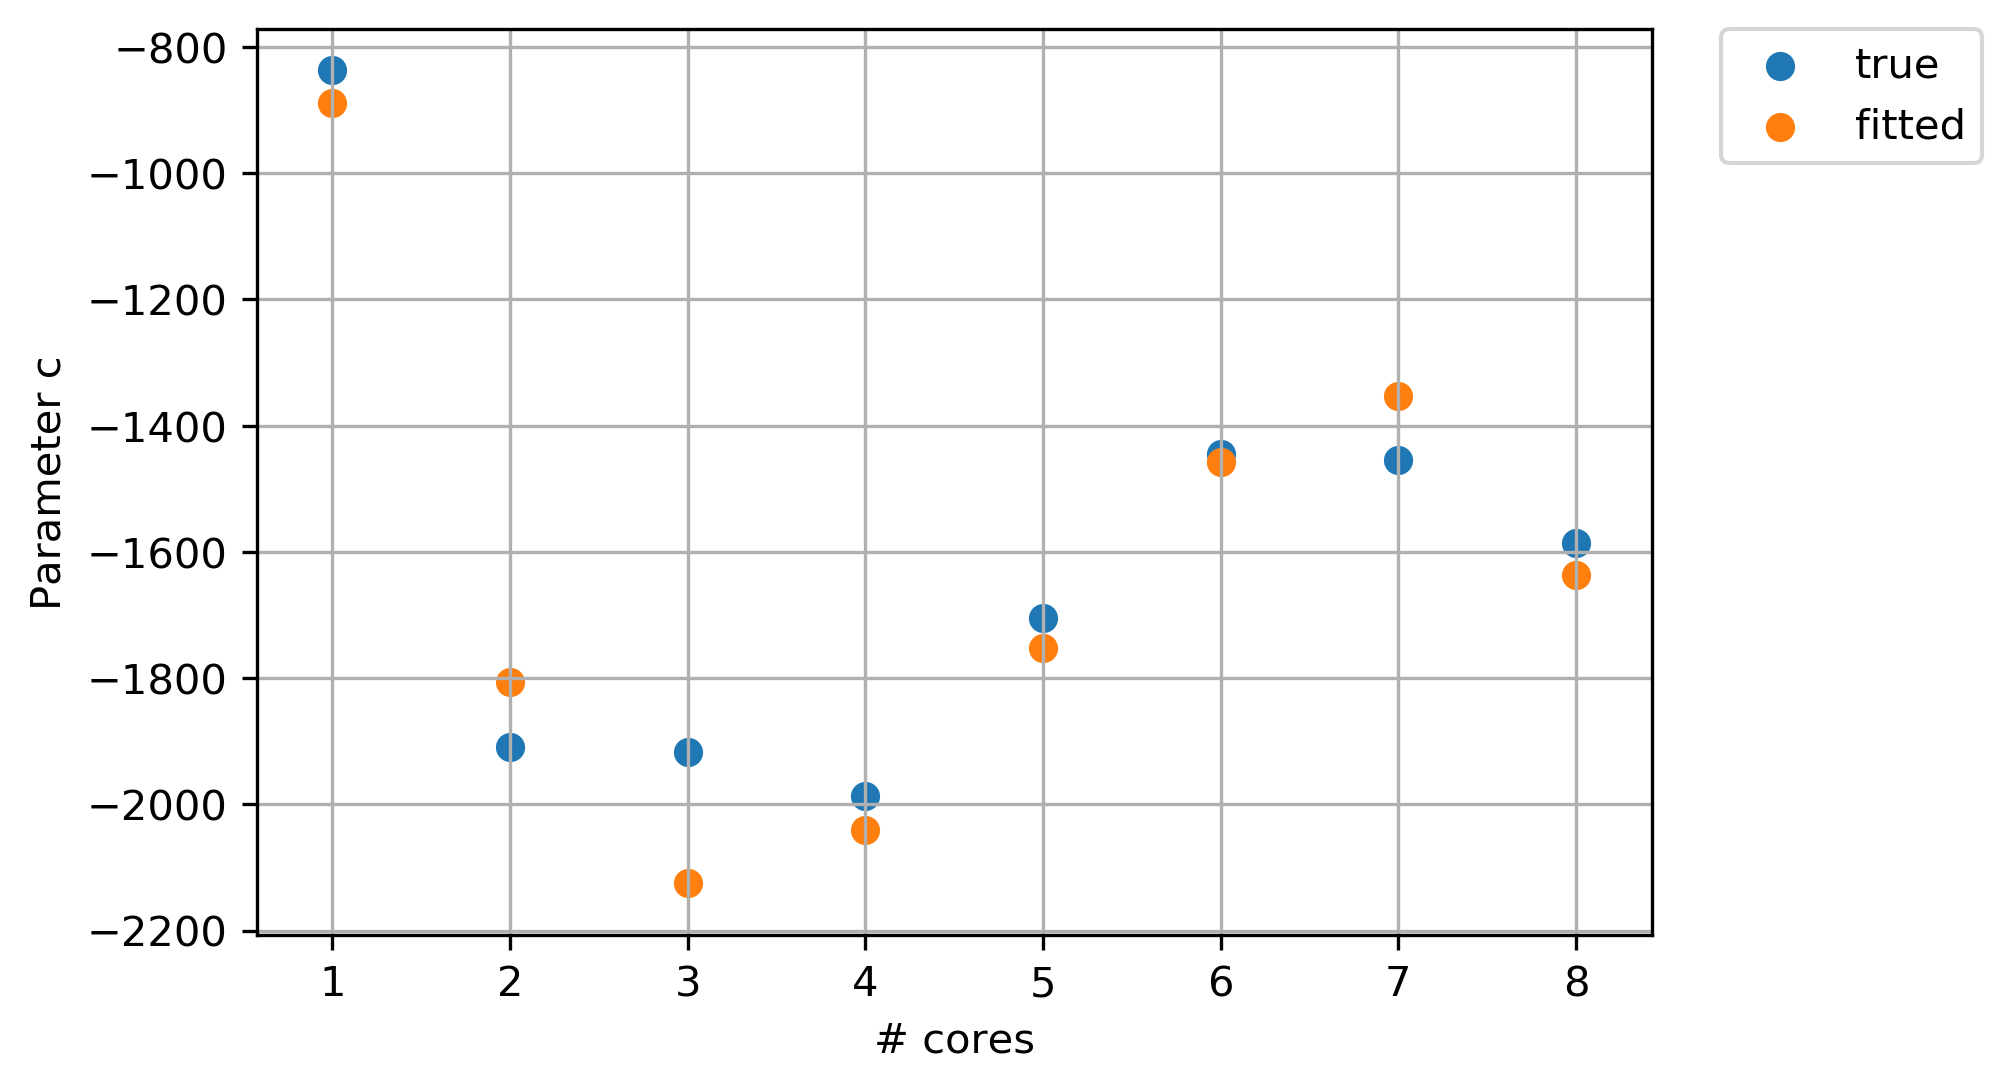
\includegraphics[scale=.25]{images/polyfit/fig_690_params_2.png}\label{fig15:c}}
			\caption{Fitting the parameters of the polynomial function with a $3$rd degree polynomial from the $DMATDMATADD$ benchmark for matrix size $1587\times1587$ against different number of cores.}	
			\label{fig15}
		\end{figure}
	\end{outline}
\end{frame}

\begin{frame}{Method: Modeling Performance based on Grain Size}
	\begin{outline}
		The final model: $$P=\sum_{i=0}^{2} \sum_{j=0}^{3}a_{ij}g^iN^j$$
	\begin{figure}[H]
		\centering
		\subfloat[]{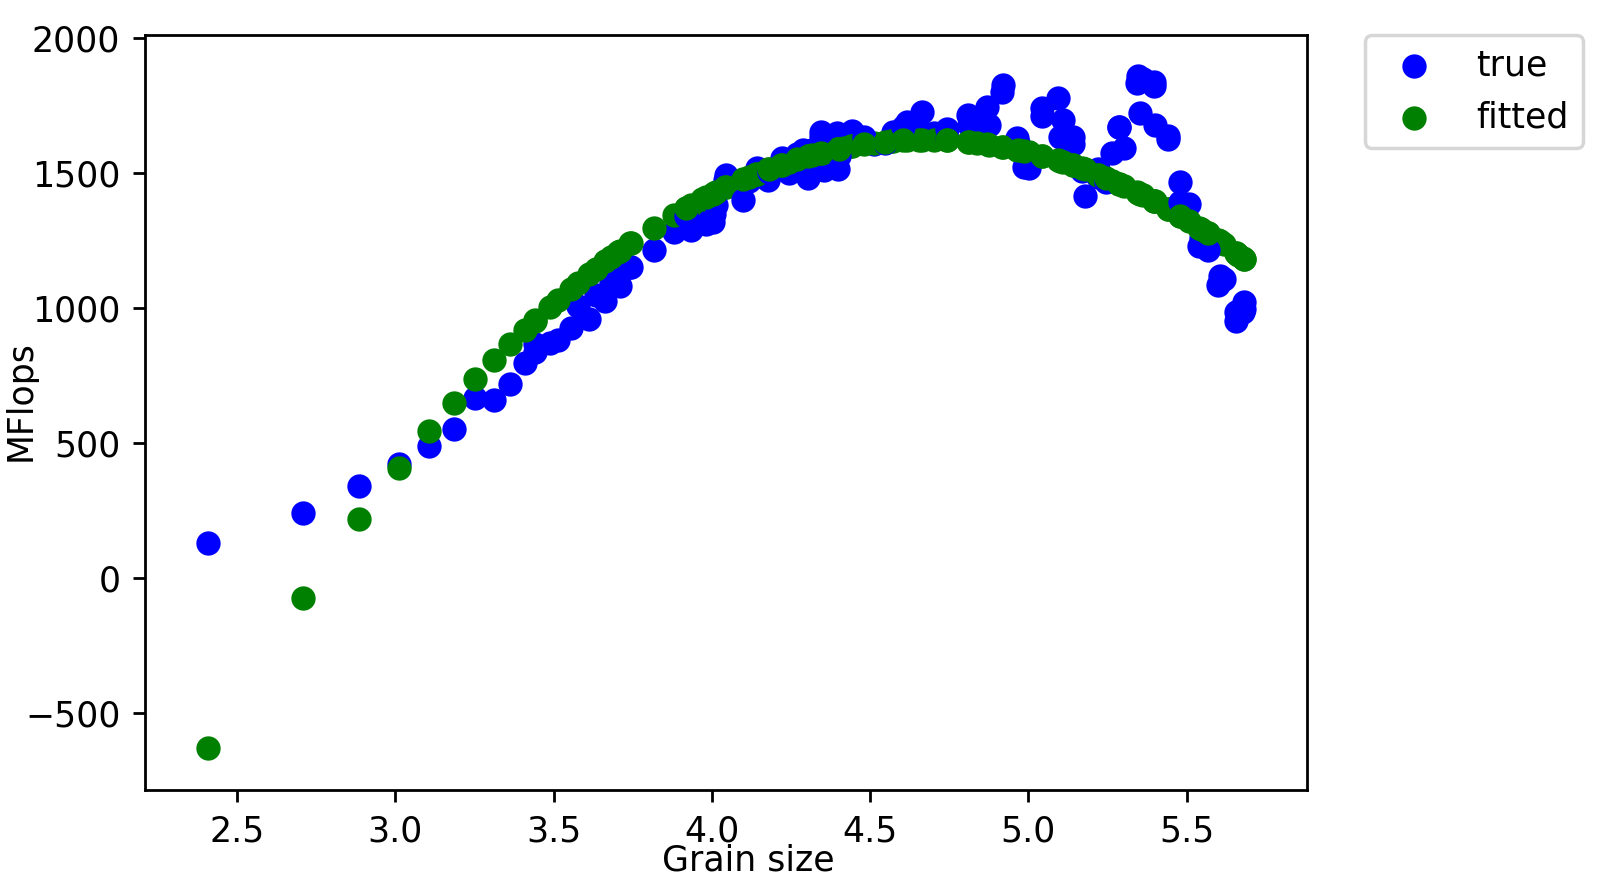
\includegraphics[scale=.25]{images/polyfit/fig_690_total_2.png}\label{fig18:a}}
		\subfloat[]{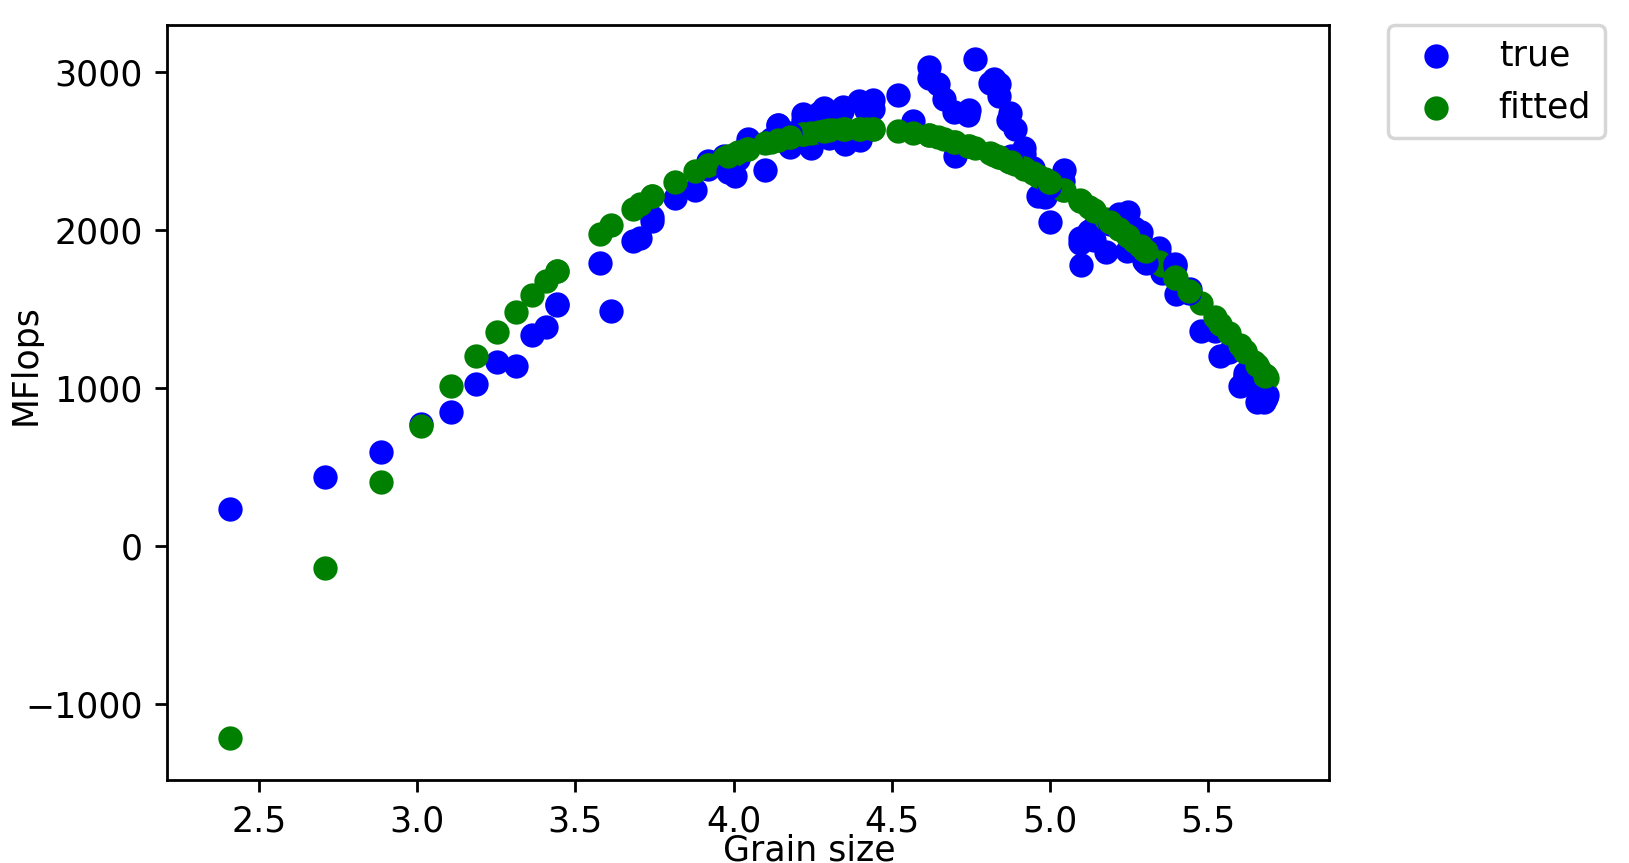
\includegraphics[scale=.25]{images/polyfit/fig_690_total_4.png}\label{fig18:b}}\hfill
		\subfloat[]{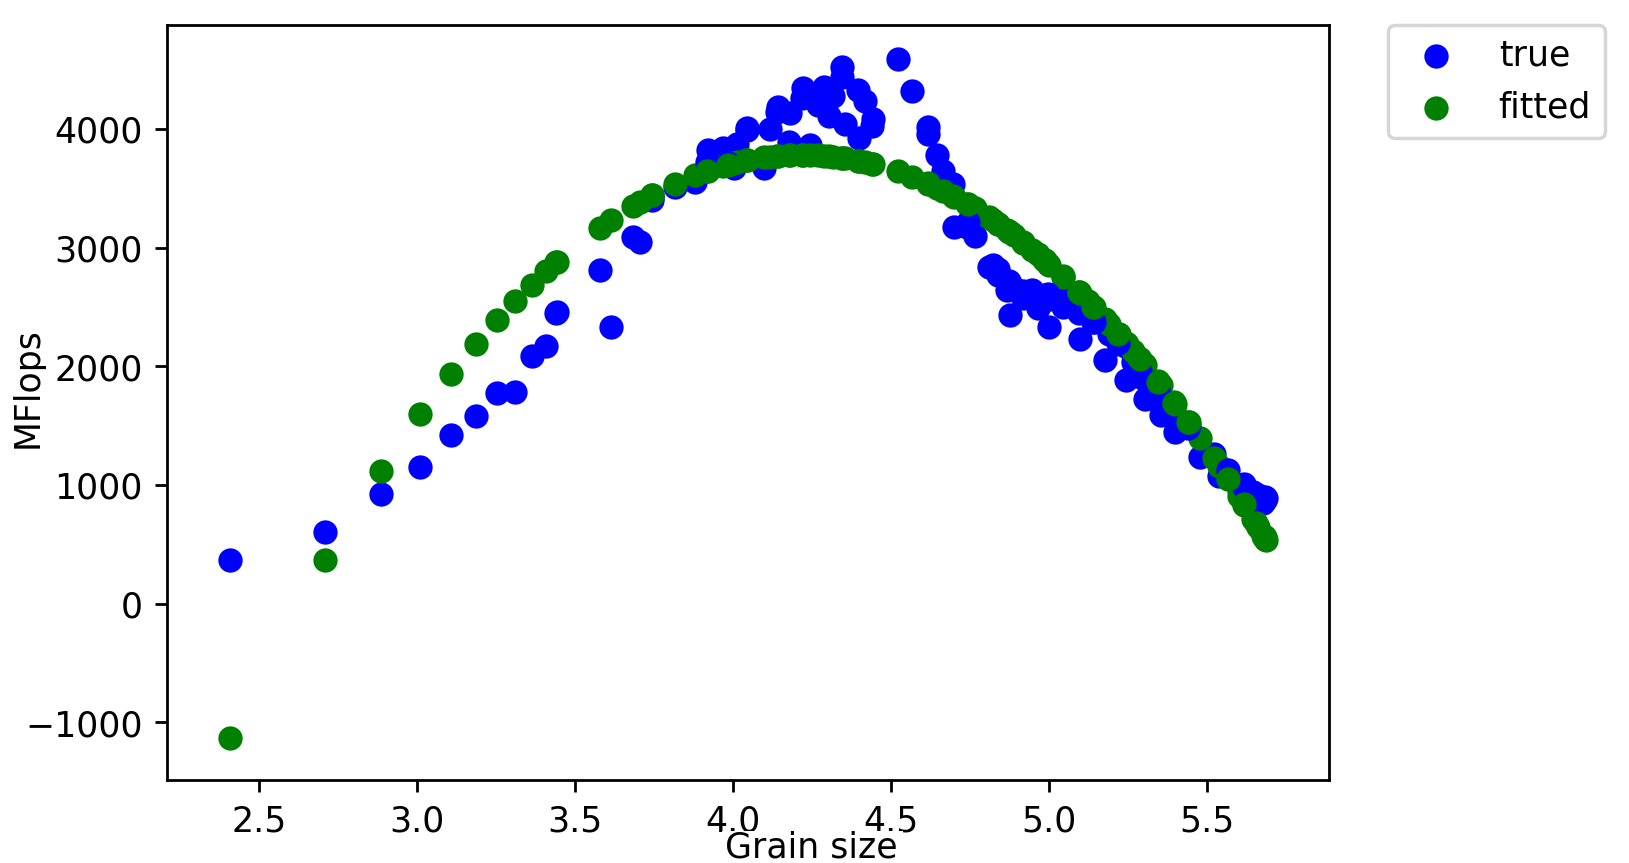
\includegraphics[scale=.25]{images/polyfit/fig_690_total_8.png}\label{fig18:c}}
		\caption{matrix size $690\times690$ for (a) 2 core, (b) 4 cores, (c) 8 cores.}	
		\label{fig18}
	\end{figure}
	\end{outline}
\end{frame}

\begin{frame}{Method: Modeling Performance based on Grain Size}
	\begin{outline}
		\begin{figure}[H]
			\centering
			{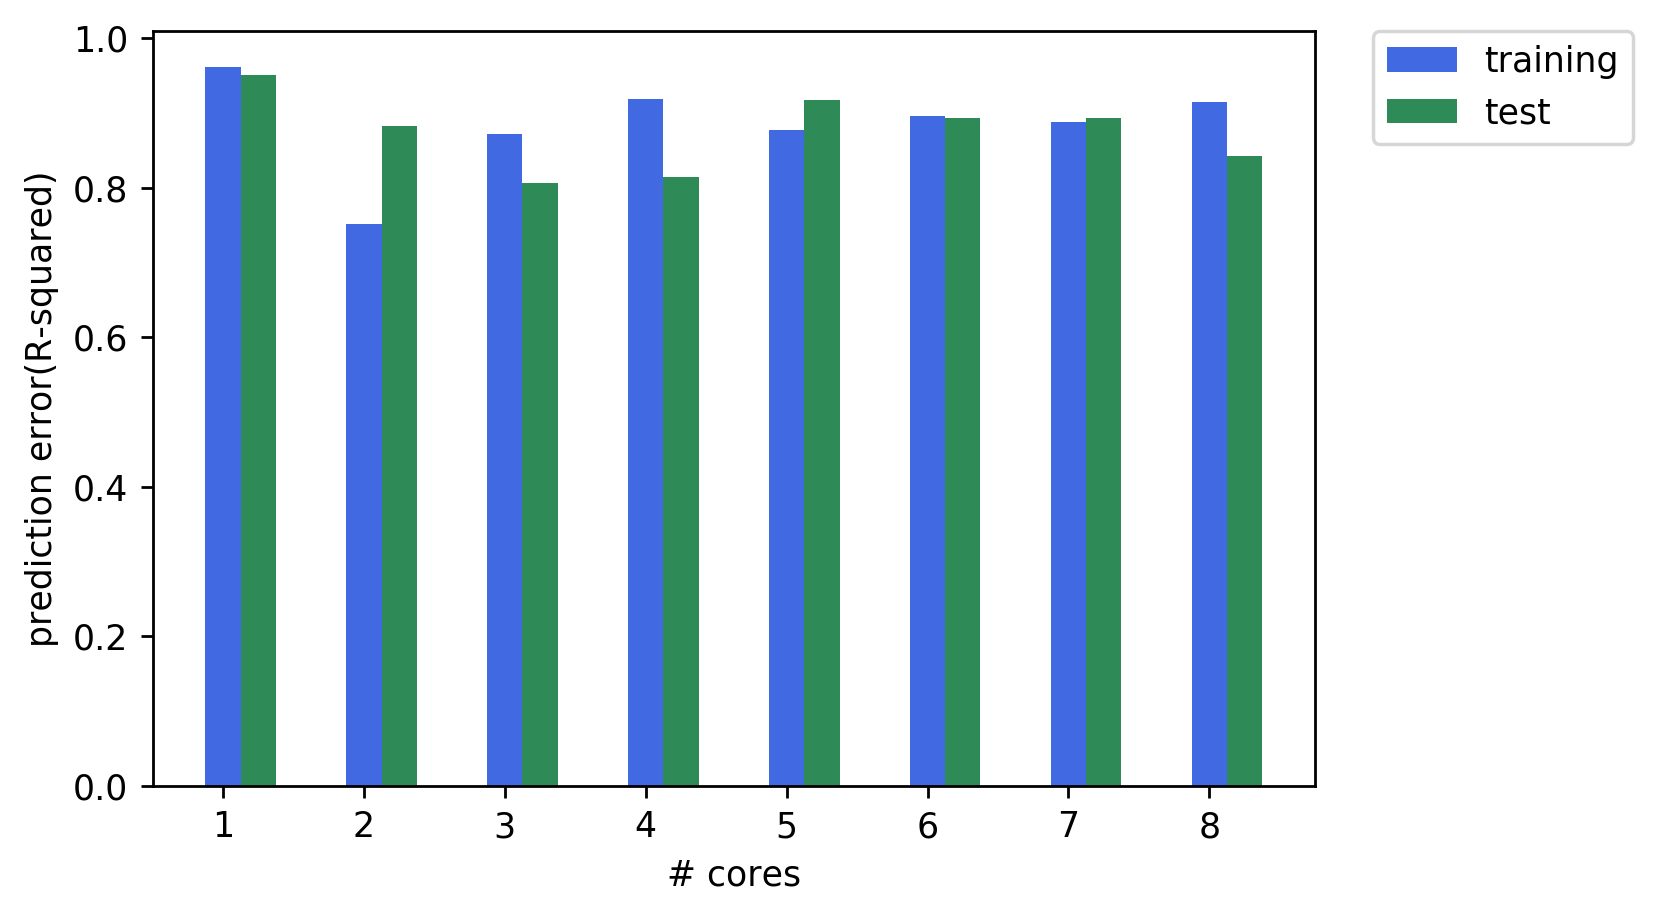
\includegraphics[scale=.32]{images/polyfit/fig_690_total_error_r2.png}\label{fig17:a}}
	
			\caption{All the data points are included in calculation of error, R\textunderscore{squared} error.}	
			\label{fig17}
		\end{figure}
	\end{outline}
\end{frame}

%\begin{frame}{Method: Modeling Performance based on Grain Size}
%	\begin{outline}
%		\begin{figure}[H]
%			\centering
%			\subfloat[]{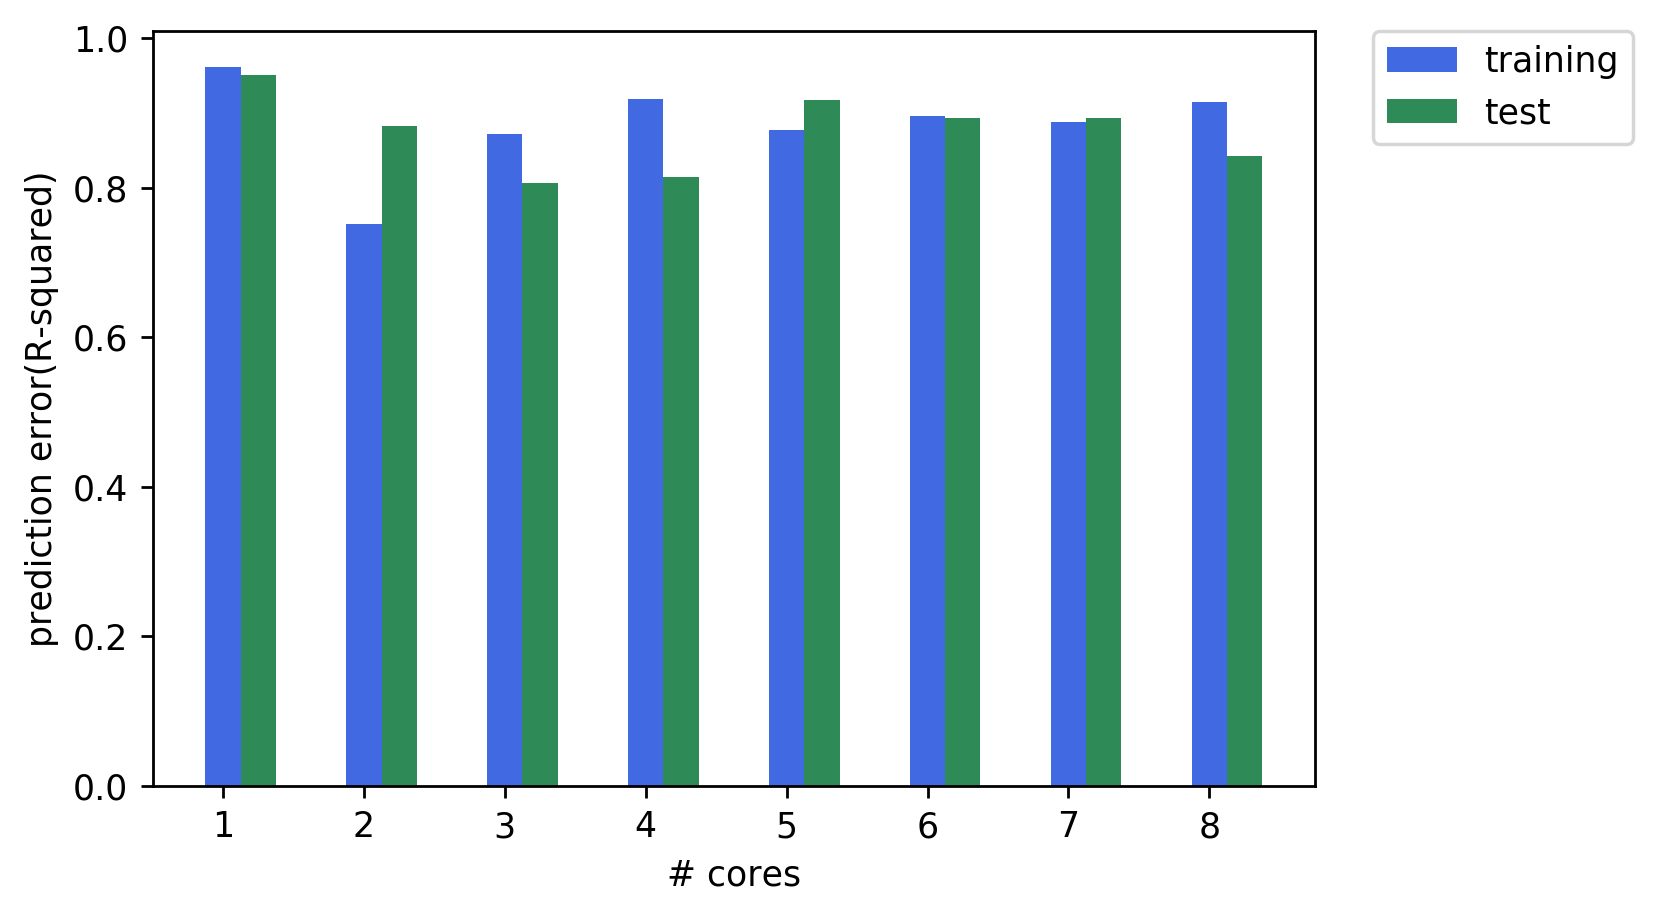
\includegraphics[scale=.32]{images/polyfit/fig_690_total_error_r2.png}\label{fig17:a}}
%			\subfloat[]{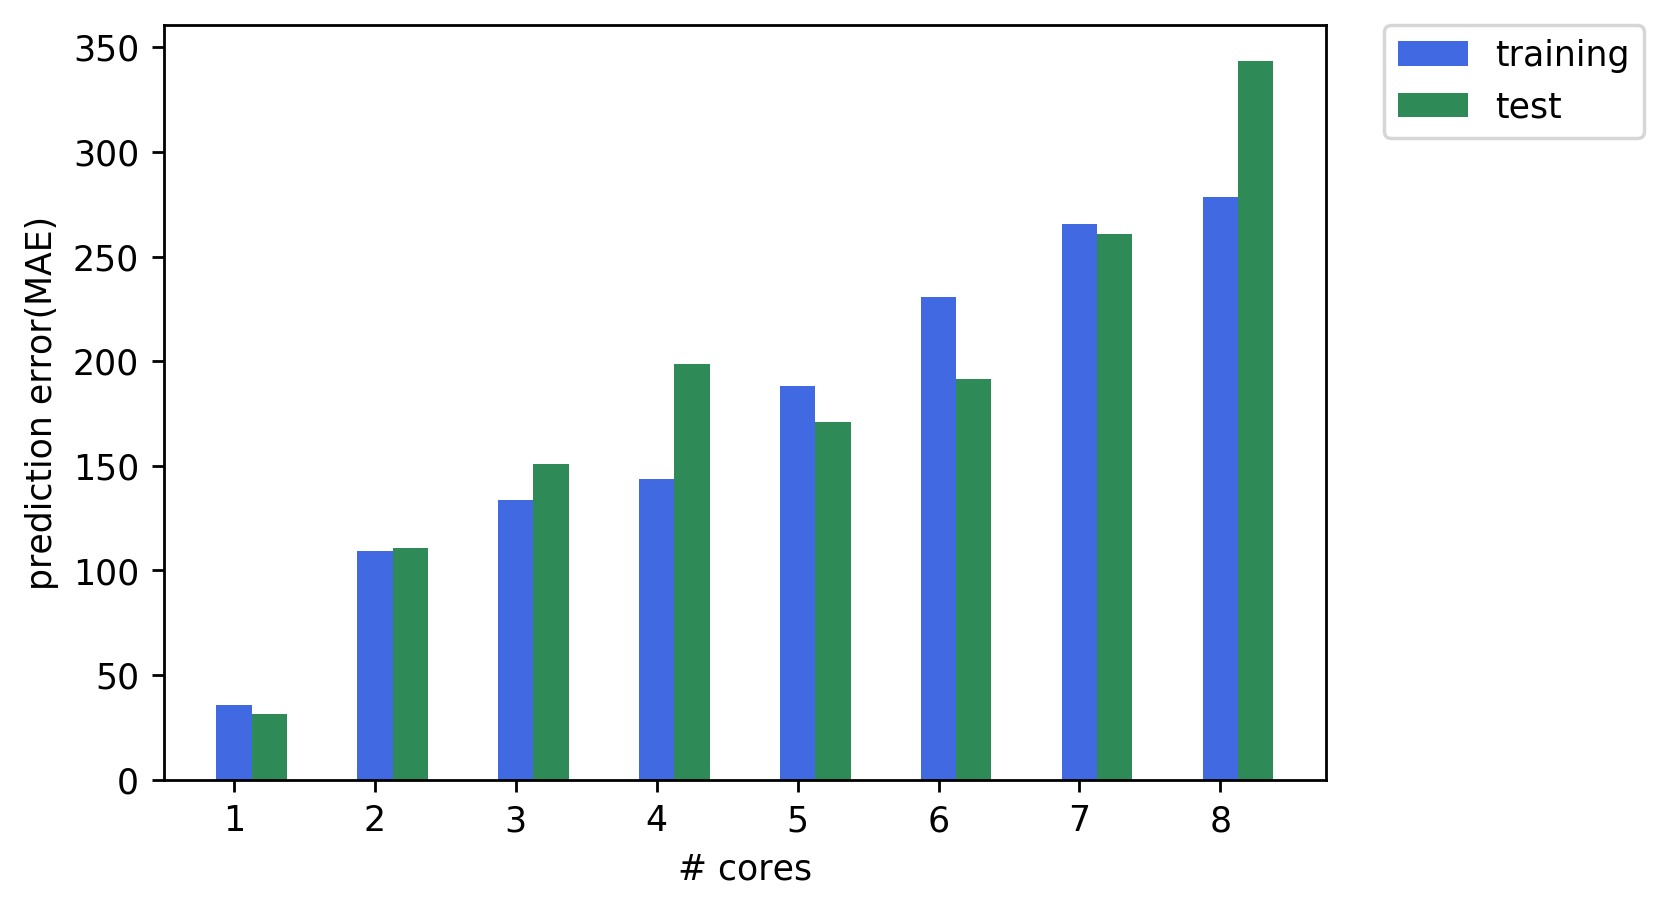
\includegraphics[scale=.32]{images/polyfit/fig_690_total_error_mae.png}\label{fig17:b}}
%			\caption{All the data points are included in calculation of error,(a) R\textunderscore{squared} error (b) Mean Absolute Error(MAE) .}	
%			\label{fig17}
%		\end{figure}
%	\end{outline}
%\end{frame}



\begin{frame}{Method: Finding the Grain Size Range for Maximum Performance}
	\begin{outline}
\begin{figure}[H]
	\centering
	\subfloat[]{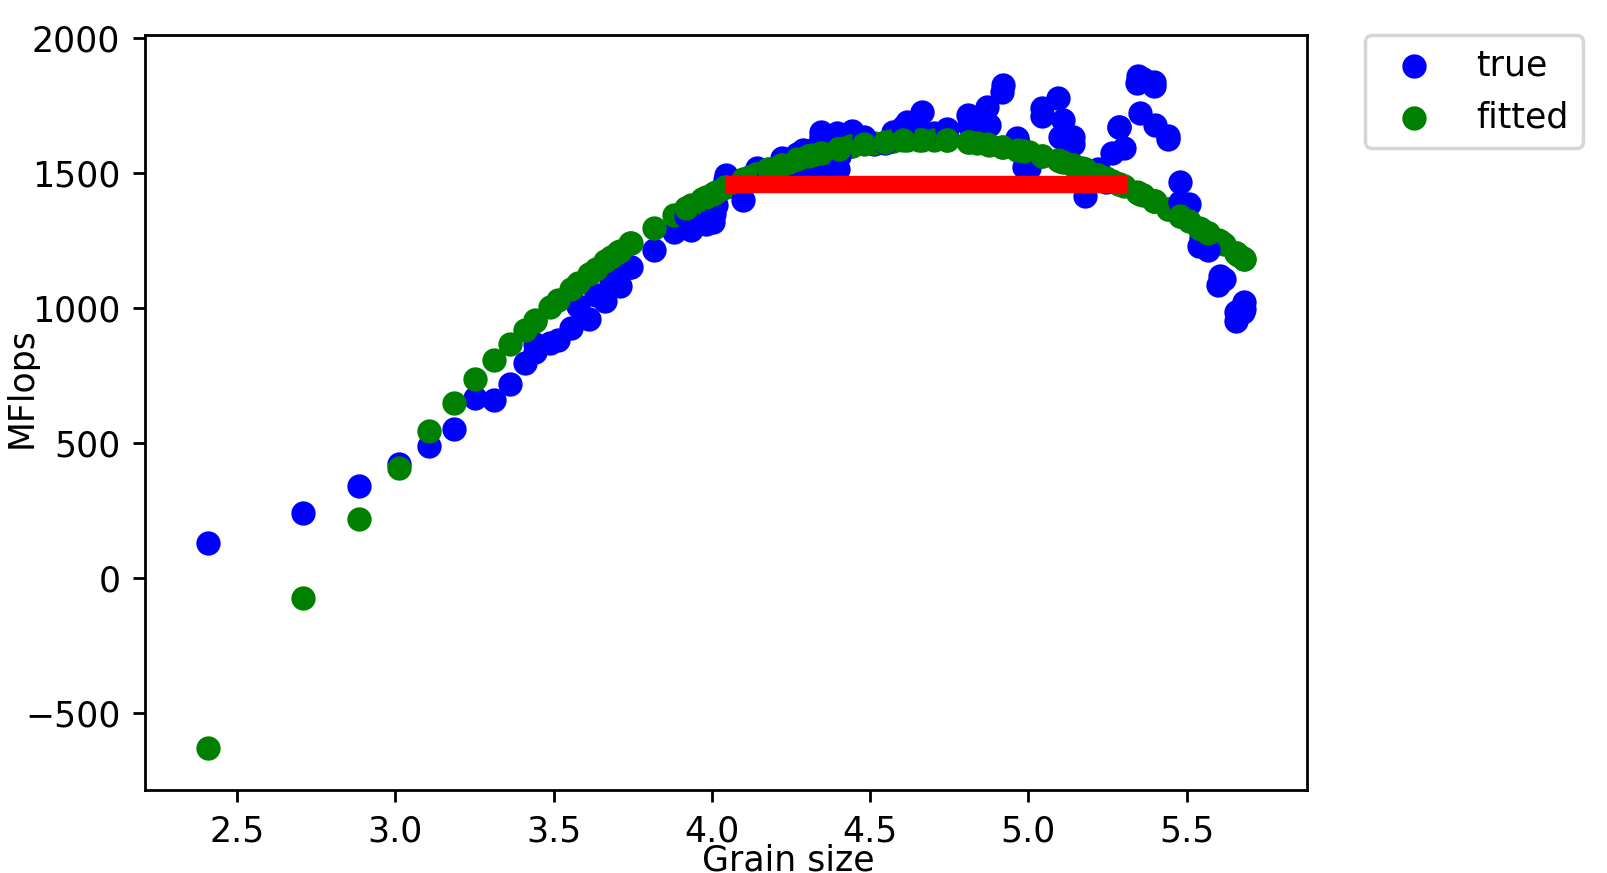
\includegraphics[scale=.3]{images/polyfit/fig_690_total_2_range.png}\label{fig12:a}}
	{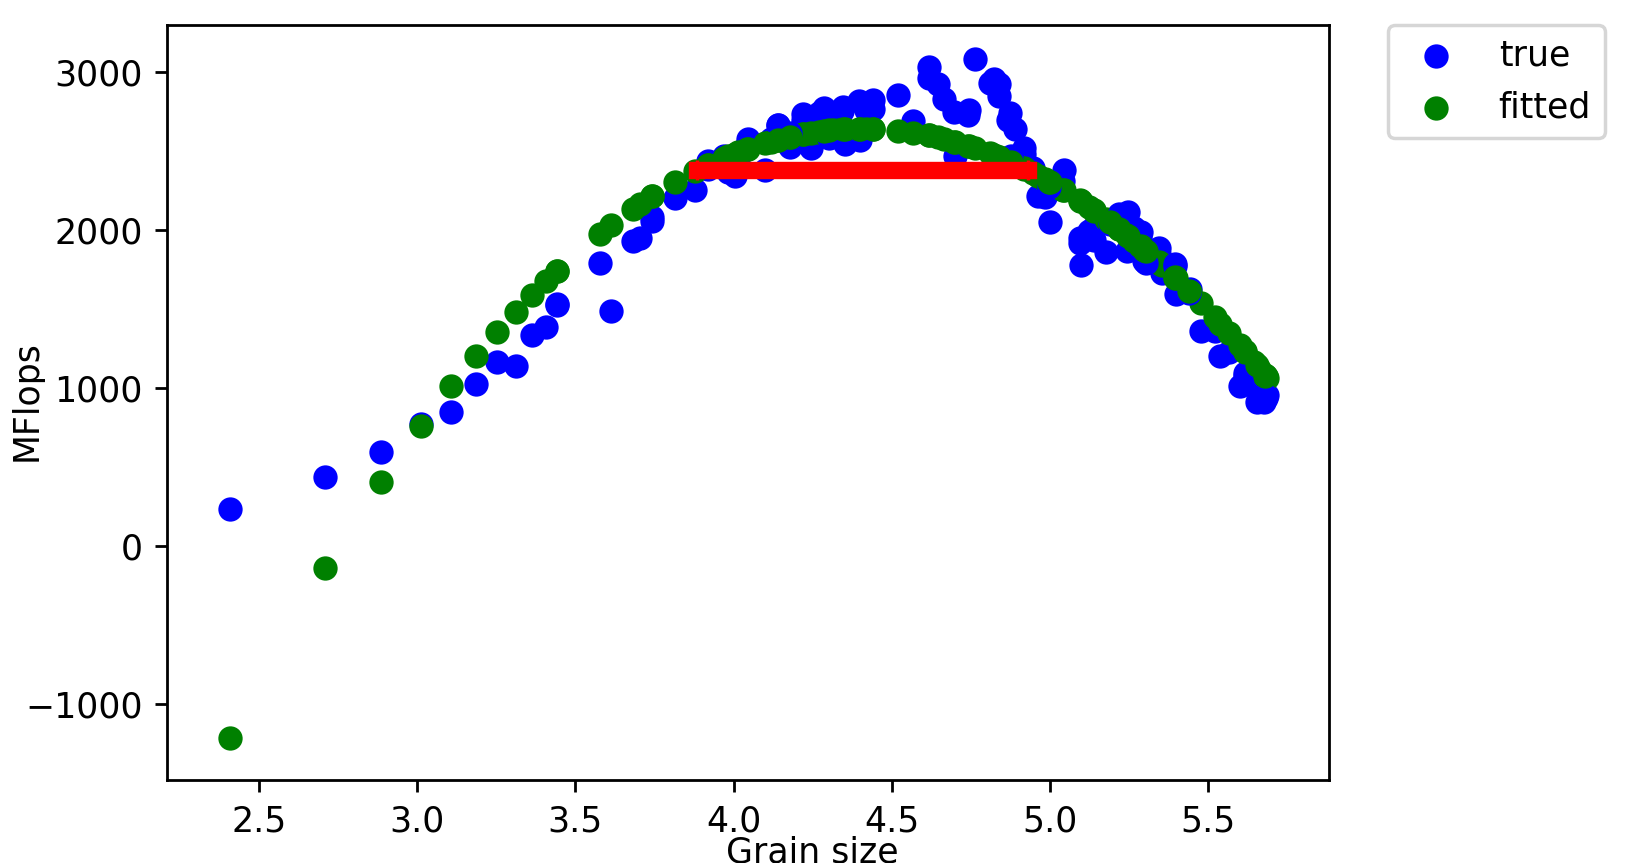
\includegraphics[scale=.3]{images/polyfit/fig_690_total_4_range.png}\label{fig12:b}}
	\subfloat[]{\includegraphics[scale=.3]{images/polyfit/fig_690_total_8_range.png}\label{fig12:c}}
	\caption{The range of grain size (shown as the red line) that leads to a performance within $10\%$ of the maximum performance for (a) 2 cores, (b) 4 cores and (b) 8 cores.}	
	\label{fig12}
\end{figure}
	\end{outline}
\end{frame}

%\begin{frame}{Method: Finding the Grain Size Range for Maximum Performance}
%	\begin{outline}
%		\begin{figure}[H]
%			\centering
%			{\includegraphics[scale=.3]{images/polyfit/fig_690_peak_range_all.png}\label{fig13:a}}
%%			{\includegraphics[scale=.3]{images/polyfit/fig_523-912_peak_range_all.png}\label{fig13:b}}
%			\caption{The range of grain size within $10\%$ of the maximum performance of the fitted polynomial function for $DMATDMATADD$ benchmark for different number of cores for (a) matrix size $690\times690$}	
%			\label{fig13}
%\end{figure}
%\end{outline}
%\end{frame}

\begin{frame}{Method: Finding the Grain Size Range for Maximum Performance}
	\begin{outline}
	How do we use the calculated range?
	\includegraphics[scale=.3]{images/polyfit/fig_690_total_8_range.png}
	\1Select a reasonable block size, e.g. $4\times512$
	\1Find the range of chunk size that results in the calculated range of grain size, Grain\textunderscore{size}=$r\times{c}\times{ch}$
	\end{outline}
\end{frame}

\begin{frame}{Method: Finding the Grain Size Range for Maximum Performance}
	\begin{outline}
		\begin{figure}[H]
			\centering
			
			\subfloat[]{\includegraphics[scale=.25]{images/polyfit/fig_690_chunks_2_4-512.png}\label{fig14:d}}
			\subfloat[]	{\includegraphics[scale=.25]{images/polyfit/fig_690_chunks_4_4-512.png}\label{fig14:e}}
			\subfloat[]{\includegraphics[scale=.25]{images/polyfit/fig_690_chunks_8_4-512.png}\label{fig14:f}}
			\caption{matrix size $690\times690$ with block size of  $4\times512$ on (a) $2$ cores, (b) $4$ cores, and (c) $8$ cores. }	
			\label{fig14}
		\end{figure}
	\end{outline}
\end{frame}

%\begin{frame}{Method: Finding the Grain Size Range for Maximum Performance}
%	\begin{outline}
%\begin{figure}[H]
%	\centering
%	\subfloat[]	{\includegraphics[scale=.25]{images/polyfit/fig_690_chunks_2_4-256.png}\label{fig14:a}}
%	\subfloat[]	{\includegraphics[scale=.25]{images/polyfit/fig_690_chunks_4_4-256.png}\label{fig14:b}}
%	\subfloat[]{\includegraphics[scale=.25]{images/polyfit/fig_690_chunks_8_4-256.png}\label{fig14:c}}\hfill
%	\subfloat[]{\includegraphics[scale=.25]{images/polyfit/fig_690_chunks_2_4-512.png}\label{fig14:d}}
%	\subfloat[]	{\includegraphics[scale=.25]{images/polyfit/fig_690_chunks_4_4-512.png}\label{fig14:e}}
%	\subfloat[]{\includegraphics[scale=.25]{images/polyfit/fig_690_chunks_8_4-512.png}\label{fig14:f}}
%	\caption{matrix size $690\times690$ with block size of $4\times256$ on (a) $2$ cores, (b) $4$ cores, and (c) $8$ cores, and block size of $4\times512$ on (d) $2$ cores, (e) $4$ cores, and (f) $8$ cores. }	
%	\label{fig14}
%\end{figure}
%\end{outline}
%\end{frame}

\begin{frame}{Method: Polynomial Model, Wrap up}
	\begin{outline}
		\0Strength:
		\1Simple model, can easily find the maximum.
		\0Weakness:
		\1It is not physical.
	\end{outline}
\end{frame}

%\begin{frame}{Method: Bathtub Model}
%	\begin{outline}
%		Can we create an analytic model for execution time based on grain size?
%	\end{outline}
%\end{frame}


%\begin{frame}{Method: Bathtub Model}
%	\begin{outline}
%\begin{figure}[H]
%	\centering
%	{\includegraphics[scale=.3]{images/bathtub/all_690_4.png}\label{fig20:a}}
%%	{\includegraphics[scale=.3]{images/bathtub/tasks_all_690_4.png}\label{fig20:b}}
%	\caption{The execution time vs. grain size graph for $DMATDMATADD$ benchmark for matrix size $690\times690$ ran on $4$ cores.}	
%	\label{fig21}
%\end{figure}
%	\end{outline}
%\end{frame}	


%\begin{frame}{Method: Bathtub Model}
%	\begin{outline}		
%		\1Overheads of creating tasks
%		\1Starvation
%		\begin{figure}
%			
%			\includegraphics[width=0.9\linewidth]{images/bathtub/all_690_4_star_over.png}	
%			\caption{Results of running the \textit{DMATDMATADD} benchmark on $8$ cores matrix size $690\times690$(time unit is microseconds)}	
%		\end{figure}
%	\end{outline}
%\end{frame}
%
%\begin{frame}{Method: Modeling Execution Time based on Grain Size}
%	\begin{outline}	
%
%		$$N\text{: Number of cores}$$	
%		$$n_t \text{: Number of created tasks}	$$
%		$$n_t=\frac{Total\:amount\:of\:work}{grain\textunderscore{size}}$$
%		$$t_s\text{: sequential execution time}$$
%		$$M\text{: Number of cores actually doing the work}$$
%
%		$$M=\left\{
%		\begin{aligned}
%		n_t  \:\:\:\:\:\:\:\:      \text{ if } n_t<N\\
%		N\:\:\:\:\:\:\:\:     \text{otherwise}
%		\end{aligned}
%		\right.$$
%		
%		\pause
%		$Execution\textunderscore{time}=\frac{t_s}{M}$
%		\pause
%		$+\alpha\frac{n_t}{M}$
%		\pause
%		$+\gamma$
%	\end{outline}
%\end{frame}
%
%\begin{frame}{Method: Modeling Execution Time based on Grain Size}
%\begin{outline}		
%	$$t=\left\{
%	\begin{aligned}
%		\alpha+\frac{t_s}{n_t}+\gamma  \:\:\:\:\:\:\:\:      \text{ if } n_t<N\\
%		\frac{\alpha{n_t}+t_s}{N}+\gamma\:\:\:\:\:\:\:\:     \text{otherwise}
%	\end{aligned}
%	\right.$$
%
%%	$$n_t \text{: number of tasks}	$$
%%	$$N\text{: number of cores}$$
%%	$$t_s\text{: sequential execution time}$$
%%	$$\gamma\text{: parallelization constant}$$
%%%	Softplus function:
%%%	$$f(x)=Ln(1+e^x)$$
%
%\end{outline}
%\end{frame}
%
%\begin{frame}{Method: Modeling Execution Time based on Grain Size}
%\begin{outline}	
%	\1Fixed matrix size, and number of cores	
%	\1Training set and test set (\%60, \%40)	
%
%	\begin{figure}[H]
%		\subfloat[]{\includegraphics[scale=.3]{images/bathtub/pred/pred_690_4.png}\label{fig22:a}} 
%		\subfloat[]{\includegraphics[scale=.3]{images/bathtub/pred/pred_690_8.png}\label{fig22:b}}	
%		\caption{The prediction of execution time based on grain size using the bathtub model, for (a)4 cores and (b)8 cores for $DMATDMATADD$ benchmark for matrix size $690\times690$.}	
%		\label{fig22}
%	\end{figure}
%\end{outline}
%\end{frame}
%
%\begin{frame}{Method: Modeling Performance based on Grain Size}
%	\begin{outline}
%		\begin{figure}[H]
%			\centering
%			\subfloat[]{\includegraphics[scale=.32]{images/bathtub/error_690r2.png}\label{fig38:a}}
%			\subfloat[]{\includegraphics[scale=.32]{images/bathtub/error_final_690mae}\label{fig38:b}}
%			\caption{The error in fitting execution time with the bathtub formula for $DMATDMATADD$ benchmark for matrix size $690\times690$ with different number of cores,(a) R\textunderscore{squared} error (b) Mean Absolute Error(MAE).}	
%			\label{fig38}
%		\end{figure}
%	\end{outline}
%\end{frame}

%\begin{frame}{Method: Modeling Execution Time based on Grain Size}
%	\begin{outline}	
%\begin{figure}[H]
%	\centering
%	{\includegraphics[scale=.45]{images/bathtub/error_690.png}}	
%	\caption{The error in fitting execution time with the bathtub formula for $DMATDMATADD$ benchmark for matrix size $690\times690$ with different number of cores.}	
%	\label{fig23}
%\end{figure}
%\end{outline}
%\end{frame}

%\begin{frame}{Method: Modeling Execution Time based on Grain Size}
%	\begin{outline}	
%	\1How do $t_s$, $\alpha$, and $\gamma$ change with number of cores?
%		$$f(N)=\frac{m_0+m_1(N-1)+m_2(N-1)N+m_3(N^2)(N-1)}{N}$$
%	\begin{figure}[]
%		\centering
%		\subfloat[]{\includegraphics[scale=.13]{images/bathtub/coef_1_690.png}\label{fig24:a}}
%		\subfloat[]{\includegraphics[scale=.13]{images/bathtub/coef_2_690.png}\label{fig24:b}}\hfill	
%		\subfloat[]{\includegraphics[scale=.13]{images/bathtub/coef_3_690.png}\label{fig24:c}}
%		\caption{Fitting the three parameters (a)$\alpha$, (b)$t_s$, and (c)$\gamma$ for $DMATDMATADD$ benchmark for matrix size $690\times690$.}	
%		\label{fig24}
%	\end{figure}
%\end{outline}
%\end{frame}


%\begin{frame}{Method: Modeling Execution Time based on Grain Size}
%	\begin{outline}	
%\begin{figure}[]
%		{\includegraphics[scale=.7]{images/bathtub/error_final_690mae.png}}	
%	\caption{The error in fitting execution time with the bathtub formula integrated with the USL modelfor $DMATDMATADD$ benchmark for matrix size $690\times690$ with different number of cores.}	
%	\label{fig25}
%\end{figure}
%\end{outline}
%\end{frame}
%
%\begin{frame}{Method: Modeling Execution Time based on Grain Size}
%	\begin{outline}	
%\1The problem with the current model is that with this formula we know that the minimum occurs at $n_t=N$.
%\1Parameters $t_s, \alpha, \gamma$ do not behave the way we expect, they change with change of number of cores.
%\\
%What is the missing factor?
%
%\end{outline}
%\end{frame}


%\begin{frame}{Modeling Execution Time based on Grain Size}
%\begin{outline}	
%	\1For a fixed matrix size, and number of cores we need 4 parameters to estimate execution time based on number of tasks
%    \1How does these four parameters change for different number of cores?
%    \2used USL to model each of these parameters
%\end{outline}
%\end{frame}



%\section{Setup}
\begin{frame}{Setup: Blazemark}
	\begin{outline}
		Blazemark is a benchmark suite provided by Blaze to compare the performance of Blaze with other linear algebra libraries. 
		\begin{figure}
			\includegraphics[width=0.42\linewidth]{images/blazemark_1.png}
			\hfill\includegraphics[width=0.41\linewidth]{images/blazemark_2.png}
			\caption{An example of results obtained from Blazemark}	
		\end{figure}
	\end{outline}
\end{frame}


\begin{frame}{Setup: Configuration}
	\begin{outline}
	\vspace{\baselineskip}	
	\begin{table}[H]
		\centering
		%	\resizebox{\textwidth}{!}
		\scalebox{0.75}
		{\begin{tabular}{|c | c |} 
				\hline
				
				Category & Specification\\
				\hline
				\hline
				CPU &  2 x Intel(R) Xeon(R) CPU E5-2450 0 @ 2.10GHz \\ [0.5ex] 
				\hline
				RAM & 48 GB\\ 	
				\hline
				Number of Cores & 16\\
				\hline	
				Hyperthreading & Off \\
				\hline			
		\end{tabular}}	
		\caption{Specifications of the Marvin node from Rostam cluster at CCT.}
		\label{table3}
	\end{table} 
\begin{table}[H]
	\centering
	%	\resizebox{\textwidth}{!}
	\scalebox{0.75}
	{\begin{tabular}{|c | c |} 
			\hline
			Library & Version \\
			\hline
			\hline
			HPX & 1.3.0 \\ 
			\hline
			Blaze & 3.5\\ 	
			\hline
			
	\end{tabular}}	
	\caption{Specifications of the libraries used to run our experiments.}
	\label{table5}
\end{table}
	\end{outline}
\end{frame}



\begin{frame}{Our Contributions}
	\begin{outline}
%		\1We propose a novel analytic model to represent how the execution time is expected to change based on grain size.
		\1To our knowledge, there has not been a work to create a 3D model of the throughput, grain size, and number of cores. 
		\1We are proposing a method to apply the developed model to a linear algebra library, in a way specific to our application, and the machine architecture.
		%Thanks to Blaze we are able to access to expression tree at compile time, through which we can estimate the complexity of the expression 
	\end{outline}
\end{frame}


\section{Future Work}
\begin{frame}{Future Work}
\begin{outline}	
	\1Generalizing the current model to different matrix sizes
	\1Looking into more complex expressions
	\1Finding an analytical model to explain the observed behavior between execution time, grain size, and number of cores.
	 
%	\begin{figure}[]
%
%
%		\subfloat[]
%		{\includegraphics[scale=.3]{images/fig11.png}	
%			\label{fig8:a}}		
%		\subfloat[]{
%			\includegraphics[scale=.3]{images/fig12.png}
%			\label{fig8:b}}
%		\caption{Throughput vs. grain size graph obtained from running $DMATDMATADD$ benchmark  on $4$ cores for matrix sizes (a) smaller than 793$\times$793 (b) larger than 793$\times$793.}
%		\label{fig20}
%	\end{figure} 
%
%	\1Studying the bathtub model to find the missing factor, also location of the minimum 
%	\1Generalization for matrix size, adding runs for larger matrix sizes
%	\1Generalization for complex expressions
%	\1Generalization for different architectures
\end{outline}
\end{frame}


\begin{frame}[standout]
  Thank you!
\end{frame}

\begin{frame}{Appendix}
	\begin{outline}	
		\begin{figure}[H]
			\includegraphics[scale=.2]{images/BLAS.png}	
			\caption{{https://web.stanford.edu/class/ee392o/nlas-foils.pdf}}
			\label{fig26}		
		\end{figure} 
	\end{outline}
\end{frame}

\begin{frame}{Appendix}
	\begin{outline}	
		\begin{figure}[H]
			\includegraphics[scale=.5]{images/polyfit/fig_523-912_peak_range_all.png} \label{fig27}	\caption{The range of grain size within $10\%$ of the maximum performance of the fitted polynomial function for $DMATDMATADD$ benchmark for different number of cores for matrix size $523\times523$ to $912\times912$.}		
		\end{figure} 
	\end{outline}
\end{frame}



\begin{frame}{Method: Modeling Performance based on Grain Size}
	\begin{outline}	
		$$Mean\textunderscore{relative\textunderscore{absolute\textunderscore{error}}} = \frac{1}{n}\sum_{i=1}^{n} abs({1-p_i/t_i})$$
		$$n \text{ is the number of samples}$$
		\begin{figure}[H]
			\centering
			\includegraphics[scale=.5]{images/polyfit/fig_train_test_690.png}
			\caption{The training and test error for fitting data obtained from the $DMATDMATADD$ benchmark for matrix size $690\times690$ against different number of cores cores.}	
			\label{fig11}
		\end{figure}
	\end{outline}
\end{frame}

\begin{frame}{Method: Modeling Performance based on Grain Size}
	\begin{outline}
		\begin{figure}[H]
			\centering
			\subfloat[]{\includegraphics[scale=.35]{images/polyfit/fig_690_total_error.png}\label{fig37:a}}
			\subfloat[]{\includegraphics[scale=.35]{images/polyfit/fig_690_total_error_corrected.png}\label{fig37:b}}
			\caption{(a) All the data points are include in calculation of error, (b) the leftmost sample was removed from error calculation.}	
			\label{fig37}
		\end{figure}
	\end{outline}
\end{frame}

\begin{frame}{Method: Bathtub Model Evaluation}
	\begin{outline}	
		\begin{figure}[H]
			\centering
			{\includegraphics[scale=.45]{images/bathtub/error_690.png}}	
			\caption{The error in fitting execution time with the bathtub formula for $DMATDMATADD$ benchmark for matrix size $690\times690$ with different number of cores.}	
			\label{fig34}
		\end{figure}
	\end{outline}
\end{frame}


	\begin{frame}{Related Work}
		\begin{outline}
			\1Liu et al. estimated the optimal number of cores to run the program on based on cache specific traces. 
			\1Khatami et al. used logistic regression to find the best chunk size based on some static and dynamic features of the loop.		
			\1Thoman et al. proposed a compile-time and runtime solution, using an effort estimation function set the chunk size. 
		\end{outline}
\end{frame}


\begin{frame}{Related Work}
	\begin{outline}	
		\begin{columns}		
			\column{0.52\linewidth}
			\begin{itemize}
\item{Laberge et al. used machine learning to find the best chunk size to get the maximum performance, while block size was fixed statistically.}
\item{Features included: matrix size, number of cores, number of floating point operations, number of iterations.} 
\end{itemize}
		\column{0.38\linewidth}
		 \begin{figure}[]
		\includegraphics[scale=.22]{images/gab.png}\caption{Laberge, G., Shirzad, S., Diehl, P., Kaiser, H., Prudhomme, S.,  Lemoine, A. (2019). Scheduling optimization of parallel linear algebra algorithms using Supervised Learning. arXiv preprint arXiv:1909.03947.}\label{fig30}
		\end{figure}
			\end{columns}	
			
	\end{outline}
\end{frame}
\begin{frame}{Method: Modeling Performance based on Grain Size}
	\begin{outline}	
		$$Mean\textunderscore{Absolute\textunderscore{Error}} = \frac{1}{n}\sum_{i=1}^{n} abs({t_i-p_i})$$
		%		$$n \text{ is the number of samples}$$
		\begin{figure}[H]
			\centering
			\includegraphics[scale=.5]{images/polyfit/error_690_mae.png}
			\caption{The training and test error for fitting data obtained from the $DMATDMATADD$ benchmark for matrix size $690\times690$ against different number of cores cores.}	
			\label{fig32}
		\end{figure}
	\end{outline}
\end{frame}
\begin{frame}{Background: Modeling Performance based on number of cores}
	\begin{outline}
		\1Amdahl's Law
		$$S(p) = \frac{p}{1+\sigma(p-1)}$$
		\1Universal Scalability Law(USL)
		%		$$X(p) = \frac{\gamma{p}}{1+\sigma(p-1)+\kappa{p}(p-1)}$$
		$$S(p) = \frac{p}{1+\sigma(p-1)+\kappa{p}(p-1)}$$
		\2 Models the effects
		of linear speedup, contention delay, and coherency delay due to crosstalk
		\begin{figure}[H]
			\centering
			\includegraphics[scale=0.38]{images/USL.png}
			\caption{An example of speedup based on Amdahl's law and USL compared to the ideal linear speedup where $\sigma=0.2$ and $\kappa=0.05$.}	
			\label{fig_Amdahl}
		\end{figure}
		
		
	\end{outline}
\end{frame}
\end{document}